% !TeX root = index.tex
\documentclass[a4paper, 14pt]{extreport}   % general format

%%%% Charset
\usepackage{cmap}							% make PDF files searchable and copyable
\usepackage[utf8]{inputenc}					% accept different input encodings
\usepackage[T2A]{fontenc}					% russian font
\usepackage[russian]{babel}					% multilingual support (T2A)


%%%% Font
\usepackage{tempora} % Time New Romans (this supports Cyrillic)
\DeclareUnicodeCharacter{0306}{}{} % й

%%%% Graphics
\usepackage[dvipsnames]{xcolor} % driver-independent color extensions
\usepackage{graphicx}           % enhanced support for graphics
\usepackage{wrapfig}            % pro­duces fig­ures which text can flow around

%%%% Math
\usepackage{amsmath}            % Amer­i­can Math­e­mat­i­cal So­ci­ety (AMS) math fa­cil­i­ties
\usepackage{amsfonts}           % fonts from the AMS
\usepackage{amssymb}            % additional math symbols

%%%% Ty­po­grapy (don't forget about cm-super)
\usepackage[left=3cm, right=1cm, top=2cm, bottom=2cm]{geometry}
\usepackage{microtype}          % sublim­i­nal re­fine­ments to­wards ty­po­graph­i­cal per­fec­tion
\linespread{1.5}                % line spacing
\setlength{\parindent}{1.25cm}     % we don't want any paragraph indentation
\usepackage{indentfirst}      % ... and after sections
\setlength{\parskip}{0cm}     % space between the paragraphs

%%%% Other
%\usepackage{hyperref}           % ver­ba­tim with URL-sen­si­tive line breaks
\usepackage[hidelinks]{hyperref}   % hide links borders
\usepackage{fancyvrb}
\usepackage{fvextra}
%\DeclareUnicodeCharacter{00A0}{~}
\usepackage{float}
\usepackage{color,soul}
\usepackage{enumitem}			% nested enumerate
\setlist[enumerate]{nosep}

%%%% Page numeration
\usepackage{fancyhdr} % Подключаем пакет fancyhdr для управления стилями колонтитулов

\fancypagestyle{clean}{ % Определяем стиль
  \fancyhf{} % Очищаем все поля колонтитулов
  \renewcommand{\headrulewidth}{0pt} % Убираем линию под заголовком
}

\fancypagestyle{plain}{ % Определяем стиль для первых страниц и всего текста
    \fancyhf{} % Очищаем заголовки и нижние колонтитулы
    \renewcommand{\headrulewidth}{0pt} % Убираем линию вверху страницы
    \fancyhead[R]{\hspace*{1cm}\thepage} % Верхний правый колонтитул с отступом
}

%\setcounter{page}{5}

%----НАЗВАНИЯ-РАЗДЕЛОВ-И-СОДЕРЖАНИЕ--------------------------------------------
\usepackage[raggedright]{titlesec} % не переносить заголовки

%\renewcommand{\chaptertitlename}{ГЛАВА}
\titleformat
	{\chapter} % command: the sectioning command to be redefined
	[block] % shape is sectioning paragraph shape
	{\centering\normalfont\normalsize\bfseries} % format: title, label, and text
%	{\chaptertitlename\ \thechapter . } % label
	{\thechapter . } % label
	{4pt} % the horizontal separation between label and title body
	{\MakeUppercase} % before-code
	[] % after-code

\titleformat{\section}[block]
{\centering\normalfont\normalsize\bfseries}{\thesection .}{4pt}{}

\titleformat{\subsection}[block]
{\centering\normalfont\normalsize}{\thesubsection .}{4pt}{}

\titleformat{\subsubsection}[block]
{\centering\normalfont\normalsize}{\thesubsubsection .}{4pt}{}

%%%% ToC
\usepackage{titletoc}

\addto\captionsrussian{% Replace "english" with the language you use
  \renewcommand{\contentsname}%
    {Содержание}%
}

\titlecontents{chapter}[0em]{}%
 {\thecontentslabel.\enspace}%numbered
 {}%numberless
 {\titlerule*[0.4pc]{.}\contentspage}%

\titlecontents{section}[0.0em]{}%
 {\thecontentslabel.\enspace}%numbered
 {}%numberless
 {\titlerule*[0.4pc]{.}\contentspage}%
 
\titlecontents{subsection}[0.0em]{}%
 {\thecontentslabel.\enspace}%numbered
 {}%numberless
 {\titlerule*[0.4pc]{.}\contentspage}%

%----СПИСОК-ИСПОЛЬЗОВАННЫХ-ИСТОЧНИКОВ------------------------------------------

%\renewcommand{\bibname}{Список использованных источников}
\addto{\captionsrussian}{\renewcommand{\bibname}{Список использованных источников}}

\urlstyle{same}

%----ЛИСТИНГ-------------------------------------------------------------------
\usepackage{listings}           % type­set source code list­ings
\usepackage{textcomp}           % for other glyphs

% Цвета для кода
\definecolor{string}{HTML}{101AF9}      % цвет строк в коде
\definecolor{comment}{HTML}{3F7F5F}     % цвет комментариев в коде
\definecolor{keyword}{HTML}{5F1441}     % цвет ключевых слов в коде
\definecolor{morecomment}{HTML}{8000FF} % цвет include и других элементов в коде
\definecolor{captiontext}{HTML}{FFFFFF} % цвет текста заголовка в коде
\definecolor{captionbk}{HTML}{999999}   % цвет фона заголовка в коде
\definecolor{bk}{HTML}{FFFFFF}          % цвет фона в коде
\definecolor{frame}{HTML}{999999}       % цвет рамки в коде

% Настройки отображения кода
\lstset{
    language=C++,               % Язык кода по умолчанию
    morekeywords={*,...},       % если хотите добавить ключевые слова, то добавляйте
    % Цвета
    keywordstyle=\color{keyword}\ttfamily\bfseries,
    stringstyle=\color{string}\ttfamily,
    commentstyle=\color{comment}\ttfamily\itshape,
    morecomment=[l][\color{morecomment}]{\#},
    % Настройки отображения
    breaklines=true,            % Перенос длинных строк
    postbreak=\raisebox{0ex}[0ex][0ex]{\ensuremath{\color{red}\hookrightarrow\space}},
    basicstyle=\ttfamily\footnotesize,    % Шрифт для отображения кода
    backgroundcolor=\color{bk}, % Цвет фона кода
    %frame=lrb,xleftmargin=\fboxsep,xrightmargin=-\fboxsep, % Рамка, подогнанная к заголовку
    frame=tblr                  % draw a frame at all sides of the code block
    rulecolor=\color{frame},    % Цвет рамки
    tabsize=2,                  % tab space width
    showstringspaces=false,     % don't mark spaces in strings
    % Настройка отображения номеров строк. Если не нужно, то удалите весь блок
    numbers=left,               % Слева отображаются номера строк
    stepnumber=1,               % Каждую строку нумеровать
    numbersep=5pt,              % Отступ от кода
    numberstyle=\small\color{black},      % Стиль написания номеров строк
    % Для отображения русского языка
    extendedchars=true,
      literate=
          {Ö}{{\"O}}1                    {Ä}{{\"A}}1                    {Ü}{{\"U}}1
          {ß}{{\ss}}1                    {ü}{{\"u}}1                    {ä}{{\"a}}1
          {ö}{{\"o}}1                    {~}{{\textasciitilde}}1        {а}{{\selectfont\char224}}1
          {б}{{\selectfont\char225}}1    {в}{{\selectfont\char226}}1    {г}{{\selectfont\char227}}1
          {д}{{\selectfont\char228}}1    {е}{{\selectfont\char229}}1    {ё}{{\"e}}1
          {ж}{{\selectfont\char230}}1    {з}{{\selectfont\char231}}1    {и}{{\selectfont\char232}}1
          {й}{{\selectfont\char233}}1    {к}{{\selectfont\char234}}1    {л}{{\selectfont\char235}}1
          {м}{{\selectfont\char236}}1    {н}{{\selectfont\char237}}1    {о}{{\selectfont\char238}}1
          {п}{{\selectfont\char239}}1    {р}{{\selectfont\char240}}1    {с}{{\selectfont\char241}}1
          {т}{{\selectfont\char242}}1    {у}{{\selectfont\char243}}1    {ф}{{\selectfont\char244}}1
          {х}{{\selectfont\char245}}1    {ц}{{\selectfont\char246}}1    {ч}{{\selectfont\char247}}1
          {ш}{{\selectfont\char248}}1    {щ}{{\selectfont\char249}}1    {ъ}{{\selectfont\char250}}1
          {ы}{{\selectfont\char251}}1    {ь}{{\selectfont\char252}}1    {э}{{\selectfont\char253}}1
          {ю}{{\selectfont\char254}}1    {я}{{\selectfont\char255}}1    {А}{{\selectfont\char192}}1
          {Б}{{\selectfont\char193}}1    {В}{{\selectfont\char194}}1    {Г}{{\selectfont\char195}}1
          {Д}{{\selectfont\char196}}1    {Е}{{\selectfont\char197}}1    {Ё}{{\"E}}1
          {Ж}{{\selectfont\char198}}1    {З}{{\selectfont\char199}}1    {И}{{\selectfont\char200}}1
          {Й}{{\selectfont\char201}}1    {К}{{\selectfont\char202}}1    {Л}{{\selectfont\char203}}1
          {М}{{\selectfont\char204}}1    {Н}{{\selectfont\char205}}1    {О}{{\selectfont\char206}}1
          {П}{{\selectfont\char207}}1    {Р}{{\selectfont\char208}}1    {С}{{\selectfont\char209}}1
          {Т}{{\selectfont\char210}}1    {У}{{\selectfont\char211}}1    {Ф}{{\selectfont\char212}}1
          {Х}{{\selectfont\char213}}1    {Ц}{{\selectfont\char214}}1    {Ч}{{\selectfont\char215}}1
          {Ш}{{\selectfont\char216}}1    {Щ}{{\selectfont\char217}}1    {Ъ}{{\selectfont\char218}}1
          {Ы}{{\selectfont\char219}}1    {Ь}{{\selectfont\char220}}1    {Э}{{\selectfont\char221}}1
          {Ю}{{\selectfont\char222}}1    {Я}{{\selectfont\char223}}1    {і}{{\selectfont\char105}}1
          {ї}{{\selectfont\char168}}1    {є}{{\selectfont\char185}}1    {ґ}{{\selectfont\char160}}1
          {І}{{\selectfont\char73}}1     {Ї}{{\selectfont\char136}}1    {Є}{{\selectfont\char153}}1
          {Ґ}{{\selectfont\char128}}1
}

\lstdefinestyle{CommandLineStyle}{
    basicstyle=\small\ttfamily,
    % basicstyle=\fontfamily{pcr}\footnotesize,
    numbers=none,
    %frame=tblr                  % draw a frame at all sides of the code block
    frame=none,                  % draw a frame at all sides of the code block
    rulecolor=\color{frame},    % Цвет рамки
    tabsize=2,                  % tab space width
    showstringspaces=false,     % don't mark spaces in strings
    columns=fullflexible,
    breaklines=true,
    breakindent=1em,
    postbreak=\raisebox{0ex}[0ex][0ex]{\ensuremath{\color{red}\hookrightarrow\space}},
    breakautoindent=true,
    literate={`}{\textasciigrave}{1}
}

% https://mysnippets443.wordpress.com/2015/11/28/latex-insert-javascript-code-with-lstlisting-package/

%Define the listing package
\usepackage{listings} %code highlighter
\usepackage{xcolor} %use xcolor
\definecolor{mygreen}{rgb}{0,0.6,0}
\definecolor{mygray}{rgb}{0.5,0.5,0.5}
\definecolor{mymauve}{rgb}{0.58,0,0.82}
 
%Customize a bit the look
\lstset{ %
backgroundcolor=\color{white}, % choose the background color; you must add \usepackage{color} or \usepackage{xcolor}
basicstyle=\footnotesize, % the size of the fonts that are used for the code
breakatwhitespace=false, % sets if automatic breaks should only happen at whitespace
breaklines=true, % sets automatic line breaking
captionpos=b, % sets the caption-position to bottom
commentstyle=\color{mygreen}, % comment style
deletekeywords={...}, % if you want to delete keywords from the given language
escapeinside={\%*}{*)}, % if you want to add LaTeX within your code
extendedchars=true, % lets you use non-ASCII characters; for 8-bits encodings only, does not work with UTF-8
frame=single, % adds a frame around the code
keepspaces=true, % keeps spaces in text, useful for keeping indentation of code (possibly needs columns=flexible)
keywordstyle=\color{blue}, % keyword style
% language=Octave, % the language of the code
morekeywords={*,...}, % if you want to add more keywords to the set
numbers=left, % where to put the line-numbers; possible values are (none, left, right)
numbersep=5pt, % how far the line-numbers are from the code
numberstyle=\tiny\color{mygray}, % the style that is used for the line-numbers
rulecolor=\color{black}, % if not set, the frame-color may be changed on line-breaks within not-black text (e.g. comments (green here))
showspaces=false, % show spaces everywhere adding particular underscores; it overrides 'showstringspaces'
showstringspaces=false, % underline spaces within strings only
showtabs=false, % show tabs within strings adding particular underscores
stepnumber=1, % the step between two line-numbers. If it's 1, each line will be numbered
stringstyle=\color{mymauve}, % string literal style
tabsize=2, % sets default tabsize to 2 spaces
title=\lstname % show the filename of files included with \lstinputlisting; also try caption instead of title
}
%END of listing package%
 
\definecolor{darkgray}{rgb}{.4,.4,.4}
\definecolor{purple}{rgb}{0.65, 0.12, 0.82}
 
%define Javascript language
\lstdefinelanguage{JavaScript}{
keywords={typeof, new, true, false, catch, function, return, null, catch, switch, var, if, in, while, do, else, case, break},
keywordstyle=\color{blue}\bfseries,
ndkeywords={class, export, boolean, throw, implements, import, this},
ndkeywordstyle=\color{darkgray}\bfseries,
identifierstyle=\color{black},
sensitive=false,
comment=[l]{//},
morecomment=[s]{/*}{*/},
commentstyle=\color{purple}\ttfamily,
stringstyle=\color{red}\ttfamily,
morestring=[b]',
morestring=[b]"
}
 
\lstset{
language=JavaScript,
extendedchars=true,
basicstyle=\footnotesize\ttfamily,
showstringspaces=false,
showspaces=false,
numbers=left,
numberstyle=\footnotesize,
numbersep=9pt,
tabsize=2,
breaklines=true,
showtabs=false,
captionpos=b
}
 % javascrypt
% Copyright 2017 Sergei Tikhomirov, MIT License
% https://github.com/s-tikhomirov/solidity-latex-highlighting/
% Copyright 2024 Semen Martynov, MIT License

\usepackage{listings, xcolor}

\definecolor{verylightgray}{rgb}{.97,.97,.97}

\lstdefinelanguage{Solidity}{
	keywords=[1]{anonymous, assembly, assert, balance, break, call, callcode, case, catch, class, constant, continue, constructor, contract, debugger, default, delegatecall, delete, do, else, emit, event, experimental, export, external, false, finally, for, function, gas, if, implements, import, in, indexed, instanceof, interface, internal, is, length, library, log0, log1, log2, log3, log4, memory, modifier, new, payable, pragma, private, protected, public, pure, push, require, return, returns, revert, selfdestruct, send, solidity, storage, struct, suicide, super, switch, then, this, throw, transfer, true, try, typeof, using, value, view, while, with, addmod, ecrecover, keccak256, mulmod, ripemd160, sha256, sha3}, % generic keywords including crypto operations
	keywordstyle=[1]\color{blue}\bfseries,
	keywords=[2]{address, bool, byte, bytes, bytes1, bytes2, bytes3, bytes4, bytes5, bytes6, bytes7, bytes8, bytes9, bytes10, bytes11, bytes12, bytes13, bytes14, bytes15, bytes16, bytes17, bytes18, bytes19, bytes20, bytes21, bytes22, bytes23, bytes24, bytes25, bytes26, bytes27, bytes28, bytes29, bytes30, bytes31, bytes32, enum, int, int8, int16, int24, int32, int40, int48, int56, int64, int72, int80, int88, int96, int104, int112, int120, int128, int136, int144, int152, int160, int168, int176, int184, int192, int200, int208, int216, int224, int232, int240, int248, int256, mapping, string, uint, uint8, uint16, uint24, uint32, uint40, uint48, uint56, uint64, uint72, uint80, uint88, uint96, uint104, uint112, uint120, uint128, uint136, uint144, uint152, uint160, uint168, uint176, uint184, uint192, uint200, uint208, uint216, uint224, uint232, uint240, uint248, uint256, var, void, ether, finney, szabo, wei, days, hours, minutes, seconds, weeks, years},	% types; money and time units
	keywordstyle=[2]\color{teal}\bfseries,
	keywords=[3]{block, blockhash, coinbase, difficulty, gaslimit, number, timestamp, msg, data, gas, sender, sig, value, now, tx, gasprice, origin},	% environment variables
	keywordstyle=[3]\color{violet}\bfseries,
	identifierstyle=\color{black},
	sensitive=true,
	comment=[l]{//},
	morecomment=[s]{/*}{*/},
	commentstyle=\color{gray}\ttfamily,
	stringstyle=\color{red}\ttfamily,
	morestring=[b]',
	morestring=[b]"
}

\lstset{
	language=Solidity,
	backgroundcolor=\color{white},
	extendedchars=true,
	basicstyle=\footnotesize\ttfamily,
	showstringspaces=false,
	showspaces=false,
	numbers=left,
	numberstyle=\footnotesize,
	numbersep=9pt,
	tabsize=2,
	breaklines=true,
	showtabs=false,
	captionpos=b
}
 % solidity

% Для настройки заголовка кода
\usepackage[labelsep=period]{caption}
%\DeclareCaptionFont{white}{\color{сaptiontext}}
\DeclareCaptionFont{white}{\color[HTML]{FFFFFF}}
%\DeclareCaptionFormat{listing}{\parbox{\linewidth}{\colorbox{сaptionbk}{\parbox{\linewidth}{#1#2#3}}\vskip-4pt}}
\DeclareCaptionFormat{listing}{\parbox{\linewidth}{\begin{flushright}
{#1#2#3}
\end{flushright}\vskip-4pt}}
\captionsetup[lstlisting]{format=listing}
\renewcommand{\lstlistingname}{Листинг}   % Переименование Listings в нужное именование структуры

%------------------------------------------------------------------------------
\begin{document}

\pagestyle{clean} % Применяем стиль plain для первой страницы
\begin{titlepage}
\begin{center} % Center everything on the page

%----------------------------------------------------------------------------------------
%    HEADING SECTIONS
%----------------------------------------------------------------------------------------

% Name of your university/college
Министерство науки и высшего образования Российской Федерации\\
Санкт-Петербургский политехнический университет Петра Великого\\
Институт компьютерных наук и кибербезопасности\\
[1.2cm]

\begin{flushleft}
    \hspace{8.5cm}РАБОТА ДОПУЩЕНА К ЗАЩИТЕ\\
    \hspace{8.5cm}ДИРЕКТОР ВШ КТиИС\\
    \hspace{8.5cm}\underline{\hspace{3.5cm}} В.А. СУШНИКОВ\\
    \hspace{8.5cm}«\underline{\hspace{1.0cm}}»\underline{\hspace{3.5cm}} 2024 г.\\[0.8cm]
\end{flushleft}

{\bfseries ВЫПУСКНАЯ КВАЛИФИКАЦИОННАЯ РАБОТА МАГИСТРА}\\[0.8cm] % Major heading such as course name
    
%----------------------------------------------------------------------------------------
%    TITLE SECTION
%----------------------------------------------------------------------------------------

{\bfseries Разработка сервиса для проведения обмена активами между\\изолированными распределёнными реестрами без установления доверия}\\[0.5cm] % Title of your document


\begin{flushleft}
	по направлению подготовки\\
	09.04.01 Информатика и вычислительная техника\\
	[-0.75cm]\underline{\hspace{17.0cm}}\\
	[-0.40cm] \hspace{3.0cm} {\small код и наименование направления подготовки (специальности)} \\
	направленность (профиль)\\
	09.04.01\_15 Технологии проектирования системного и прикладного\\
	[-0.75cm]\underline{\hspace{17.0cm}}\\
	[-0.40cm] \hspace{2.0cm} {\small код и наименование направленности (профиля) образовательной программы}\\
	программного обеспечения\\
	[-0.75cm]\underline{\hspace{17.0cm}}
\end{flushleft}
%----------------------------------------------------------------------------------------
%    AUTHOR SECTION
%----------------------------------------------------------------------------------------


\begin{flushleft}
    Выполнил\\студент гр. 5140901/21501 \hspace{3.0cm} \underline{\hspace{3cm}} \hspace{0.7cm} {С.А. Мартынов} % Your name

    Руководитель\\ доцент, к.т.н. \hspace{5.8cm} \underline{\hspace{3cm}} \hspace{0.7cm} {А.В. Самочадин} % Supervisor's Name

    Консультант по нормоконтролю\\ доцент, к.т.н. \hspace{5.8cm} \underline{\hspace{3cm}} \hspace{0.7cm} {А.Г. Новопашенный} % Supervisor's Name
\end{flushleft}

\vspace{0.3cm}
% If you don't want a supervisor, uncomment the two lines below and remove the section above
%\Large \emph{Author:}\\
%John \textsc{Smith}\\[3cm] % Your name

%----------------------------------------------------------------------------------------
%    DATE SECTION
%----------------------------------------------------------------------------------------
\centering{
    Санкт-Петербург\\
    2024
}
%----------------------------------------------------------------------------------------
%    LOGO SECTION
%----------------------------------------------------------------------------------------

%\includegraphics{Logo}\\[1cm] % Include a department/university logo - this will require the graphicx package

%----------------------------------------------------------------------------------------

\vfill % Fill the rest of the page with whitespace
\end{center}
\end{titlepage}
                            % inclide the title page
\begin{center}
\hyphenpenalty=10000 % disable sloppy
%----------------------------------------------------------------------------------------
%    HEADING SECTIONS
%----------------------------------------------------------------------------------------

% Name of your university/college
Министерство науки и высшего образования Российской Федерации\\
Санкт-Петербургский политехнический университет Петра Великого\\
Институт компьютерных наук и кибербезопасности\\
[1.2cm]

\begin{flushleft}
    \hspace{8.5cm}УТВЕРЖДАЮ\\
    \hspace{8.5cm}ДИРЕКТОР ВШ КТиИС\\
    \hspace{8.5cm}\underline{\hspace{3.5cm}} В.А. СУШНИКОВ\\
    \hspace{8.5cm}«\underline{\hspace{1.0cm}}»\underline{\hspace{3.5cm}} 2024 г.\\[0.8cm]
\end{flushleft}

ЗАДАНИЕ\\
на выполнение выпускной квалификационной работы магистра\\[1.0cm]

Студенту Мартынов Семён Андреевичу, группа 5140901/21501\hspace{1cm}\\[0.8cm]


\begin{enumerate}[label*=\arabic*.]
\item Тема работы: «Разработка сервиса для проведения обмена активами между изолированными распределёнными реестрами без установления доверия»
\item Срок сдачи студентом законченной работы: 22.05.2024
\item Исходные данные по работе:
	\begin{enumerate}[label*=\arabic*.]
	\item Материалы по работе распределённым реестрам, их видам и стандартам.
	\item Документация по работе виртуальной машины EVM в блокчейн сети Ethereum.
	\item Черновик предложения по использованию атомарных свапов в блокчейн сети Биткоин.
	\end{enumerate}
\item Содержание работы (перечень подлежащих разработке вопросов):
	\begin{enumerate}[label*=\arabic*.]
	\item Обзор существующих решений, включая исследование вопроса доверия между сторонами
	\item Формирование требований и ограничений к прототипу
	\item Описание бизнес-логики и архитектуры решения
	\item Программная реализация прототипа
	\item Модульное и системное тестирование
	\end{enumerate}
\item Консультанты по работе:\\ консультант по нормоконтролю – А.Г.Новопашенный
\item Дата выдачи задания 25.04.2024
\end{enumerate}

\vspace{0.5cm}

\begin{flushleft}
Руководитель ВКР \hspace{2.7cm} \underline{\hspace{3cm}} \hspace{0.4cm} к.т.н., доцент А.В. Самочадин

\vspace{0.5cm}

Задание принял к исполнению 25.04.20024\\
Студент \hspace{5.0cm} \underline{\hspace{3cm}} \hspace{0.4cm} С.А. Мартынов

\end{flushleft}
\end{center}
\newpage

\begin{center}
\textbf{РЕФЕРАТ}
\end{center}
\vspace{4pt}

На 127 с., 6 рисунков

\noindent ОБМЕН АКТИВАМИ, РАСПРЕДЕЛЁННЫЕ РЕЕСТРЫ, БЛОКЧЕЙН, ДОВЕРИЕ, ИНТЕРОПЕРАБЕЛЬНОСТЬ, АТОМАРНЫЙ СВОП, HTLC, ETHEREUM, BITSHARES, REACT.

\vspace{4pt}

Тема выпускной квалификационной работы: "Разработка сервиса для проведения обмена активами между изолированными распределёнными реестрами без установления доверия".

В рамках работы проведено исследование технологии распределенных реестров (DLT), включая технологию блокчейн, и изучены различные механизмы решения проблемы интеропребельности блокчейнов в части обмена активами между различными блокчейн-сетями.

Результаты ВКР:
\begin{enumerate}
\item Изучены существующие методы обмена активами и выявлены их ограничения в контексте безопасности и необходимости доверия между сторонами.
\item Создан прототип сервиса, для обмена активами между блокчейнами.
\item Проведено модульное и системное тестирование, подтверждающее работоспособность и безопасность разработанного сервиса.
\end{enumerate}

Разработанный сервис и результаты анализа могут быть использованы в финансовых организациях, работающих с международными расчётами и нуждающихся в альтернативных механизмах расчётов, либо в проектах, связанных с децентрализованными финансами (DeFi), для обеспечения более предсказуемых механизмов при проведении сделок.

Разработанный сервис показал высокую эффективность и безопасность в обмене активами между изолированными распределёнными реестрами. Это делает предложенный подход перспективным для широкого применения в различных сферах, связанных с блокчейн-технологиями и децентрализованными финансами.
\begin{center}
\textbf{THE ABSTRACT}
\end{center}
\vspace{4pt}

127 pages, 6 pictures

\noindent ASSET EXCHANGE, DISTRIBUTED LEDGERS, BLOCKCHAIN, TRUST,\\
INTEROPERABILITY, ATOMIC SWAP, HTLC, ETHEREUM, BITSHARES, REACT.

\vspace{4pt}

Topic of the graduation thesis: "Development of a service for asset exchange between isolated distributed ledgers without establishing trust."

As part of the work, research was conducted on distributed ledger technology (DLT), including blockchain technology, and various mechanisms for solving the interoperability problem of blockchains in terms of asset exchange between different blockchain networks were studied.

Thesis results:
\begin{enumerate}
\item Existing methods of asset exchange were studied and their limitations in the context of security and the need for trust between parties were identified.
\item A prototype service was created for asset exchange between blockchains.
\item Modular and system testing was conducted, confirming the operability and security of the developed service.
\end{enumerate}

The developed service and analysis results can be used in financial organizations involved in international settlements and needing alternative settlement mechanisms ori n projects related to decentralized finance (DeFi) to ensure more predictable mechanisms when conducting transactions.

The developed service demonstrated high efficiency and security in asset exchange between isolated distributed ledgers. This makes the proposed approach promising for widespread use in various fields related to blockchain technologies and decentralized finance.

\newpage
%\input{abbreviations}

\pagestyle{plain}
\tableofcontents
\sloppy  % Активируем переносы

\chapter*{Введение}
\addcontentsline{toc}{chapter}{Введение}

В последние годы технология распределённых реестров (DLT), произвела революцию в корпоративном управлении, предоставив новые возможности для децентрализованного управления процессами. Постепенно, эта технология находит своё место и в государственном управлении. Блокчейн, как частный случай DLT, изменил подход к хранению и передаче ценностей, обеспечив безопасность и прозрачность транзакций без необходимости в центральных посредниках. Это привело к появлению множества криптовалют и децентрализованных приложений, которые используют блокчейн для различных целей — от финансовых операций до распределённого управления сообществами.

Несмотря на стремительное развитие и внедрение блокчейн-технологий, возникает проблема фрагментации. Множество независимых блокчейнов создают ситуацию, в которой каждая сеть становится изолированным островом, и обмен активами между этими сетями представляет значительные сложности. В настоящий момент предложено несколько технологий, которые призваны решить (или частично решить) эту проблему. Каждый подход обладает своими сильными и слабыми сторонами.

Исследование методов и процессов обмена активами посредством атомарных свопов имеет критическое значение для дальнейшего развития блокчейн-индустрии. Это позволяет блокчейнам взаимодействовать друг с другом, не оставаясь разрозненными системами, что способствует росту и интеграции всей экосистемы.

Вопрос доверия всегда был ключевым аспектом в финансовых транзакциях. Традиционные системы полагаются на централизованные институты, такие как банки, для обеспечения доверия между сторонами. Блокчейн, благодаря своей децентрализованной природе и криптографическим механизмам, предлагает альтернативу, где доверие обеспечивается технологией, а не институтами. Атомарные свопы являются ярким примером такой технологии, которая устраняет необходимость в доверии, предоставляя безопасный и автоматизированный способ обмена активами.

Целью данной работы является разработать сервис, который бы позволил сторонам производить обмен активами между изолированными распределёнными реестрами без установления доверия. Достижение этой задачи возможно при условии исключения из сделки третьих сторон, использование децентрализованных сервисов не имеющих единой точки отказа или подверженной какому либо давлению, а так же полная прозрачность для сторон сделки.

Научная новизна работы заключается в реализации прототипа сервиса, который демонстрирует возможность проведения безопасного и эффективного обмена активами между двумя различными изолированными блокчейн сетями без установления доверия.

Практическая значимость работы заключается в том, что разработанный прототип может стать основой для создания полноценного сервиса, который позволит пользователям обмениваться активами между различными блокчейнами без необходимости доверять третьей стороне.

В этой работе решены следующие вопросы:
\begin{enumerate}
\item Обзор технологии распределённых реестров и её влияние на различные индустрии.
\item Описание проблемы фрагментации блокчейнов и необходимости межсетевого взаимодействия.
\item Обзор и выявление сильных/слабых сторон существующих технических решений обеспечения интероперабельности блокчейнов.
\item Детальное объяснение концепции атомарных свопов и их роли в блокчейн-экосистеме.
\item Пошаговый процесс проведения атомарного свопа между двумя участниками на тестовых сетях.
\item Анализ преимуществ и ограничений использования атомарных свопов.
\item Исследование аспектов доверия в контексте децентрализованных финансовых операций.
\item Оформление требований к поставленной задаче и проектирование архитектуры сервиса;
\item Выбор и обоснование технического стека для решения задачи построения сервиса;
\item Разработка сервиса проведения обмена и детальный разбор его исходного кода;
\item Тестирование сервиса.
\end{enumerate}

В конце работы обозначены вопросы, которые могут стать основой для дальнейших исследований.
\chapter{Основные понятия и возможности распределённых реестров}

В разделе приведены основные понятия распределённых реестров (и технологии блокчейн, как честного случая), рассмотрены случаи применения распределённых решений в различных отраслях, а так же проведён краткий анализ возможностей и ограничений технологии. Особое внимание уделено проблеме интероперабельности сетей.

\section{Распределенные реестров и их влияние на различные отрасли}

Существующие на данный момент централизованные бизнес-реестры данных демонстрируют ряд недостатков, препятствующих эффективному функционированию современных бизнес-процессов. Низкая эффективность существующих реестров обусловлена их сложной структурой, что приводит к повышенным затратам на их поддержку и обслуживание. Высокая стоимость создания и поддержания реестров делает их недоступными для многих участников бизнес-процессов. Отсутствие прозрачности в процессе управления реестрами создает риски неправильного использования данных, в т.ч. случаи незаконного получения доступа к данным (утечки), что подрывает доверие к реестрам и увеличивает риски для бизнеса. Разрозненность реестров в системах разных участников бизнес-процессов приводит к несогласованности данных, что усложняет принятие информированных решений. Ошибки в данных из-за отсутствия синхронизации могут привести к неверным решениям и ущербу для бизнеса. Споры, возникающие из-за недостоверности данных, требуют дорогостоящих процедур урегулирования с привлечением аудиторов, что увеличивает затраты для участников бизнес-процессов\cite{label30}.

Технологии распределенных реестров (Distributed Ledger Technologies, DLT) представляют собой инновационную парадигму децентрализованного хранения и управления информацией. DLT системы функционируют на основе распределенной сети узлов, каждый из которых обладает идентичной копией реестра, исключая централизованный контроль\cite{label39}.

Когда мы говорим о любой распределённой системе, мы сталкиваемся с классическим набором ограничений -- узлы сети могут испытывать задержки в передаче данных, периодически становиться недоступными и даже проявлять злонамеренное поведение, посылая некорректные пакеты данных. Несмотря на эти потенциальные проблемы, распределённый реестр обязан обеспечивать консистентность сети, при условии, что большинство узлов функционируют корректно и имеют согласованную точку зрения на журнал событий\cite{label15}.

Для иллюстрации рассмотрим взаимодействие между крупным металлургическим заводом и нефтегазовой компанией. Завод производит трубы по заказу компании, качество которых фиксируется в специализированной системе. Далее трубы транспортируются по железной дороге, и оператор перевозок регистрирует их в своей системе. По прибытии трубы снова проходят проверку, результаты которой заносятся в соответствующую систему. На складе их статус также фиксируется. В итоге, в процессе участвует множество промежуточных систем (таких как Контур, 1C), что делает автоматизацию этого взаимодействия достаточно обоснованным.

Один из возможных подходов для решения этой задачи -- использование стандартных интеграций вида «точка-точка» (peer-to-peer) с каждым контрагентом. В случае с одним заводом и одной нефтегазовой компанией требуется одна интеграция. С добавлением транспортной компании количество интеграций увеличивается до трёх. По мере роста числа участников количество интеграций возрастает по формуле $ \frac{n(n-1)}{2} $, где $ n $ -- число участников. Ситуацию осложняет и тот факт, что многие системы на рынке не предусматривают единый формат передачи полных данных. Полные данные можно получить через API-интерфейс, а это подразумевает написание различных решений по интеграции. Крупные компании часто тратят годы и значительные ресурсы на такие проекты. Но с развитием бизнеса, подход "точка-точка" становится всё более громоздким, и покрыть все возможные случаи кодом становится сложнее, что приводит к необходимости решать проблемы через электронную почту, телефон и прочие средства.

Альтернативным подходом состоит в использовании единой базы данных в облаке (удалённом хранилище). В этом сценарии завод, нефтегазовая компания и другие контрагенты могли бы добавлять данные о трубах и изменять их статусы. Этот подход решает проблему согласования данных, но создаёт новые вопросы: кто будет отвечать за данные? Как быть с коммерческой тайной? Можно ли доверять облачному провайдеру? Участники готовы нести ответственность за свои данные, но редко доверяют их другим, особенно крупные компании, предпочитающие закрытые системы (не говоря о компаниях, которые должны охранять свои данные по закону).

Третий подходов к решению этой задачи это использование отраслевого решения от специализированной компании-разработчика, утверждающей, что она может решить все задачи, связанные с бизнес-процессами. В этом случае все взаимодействие будет происходить через одного поставщика решений. Большинство интеграций, включающих множество участников, реализуются именно через таких сервис-провайдеров. Однако возникает проблема выбора подходящего поставщика услуг. Например, при обмене кредитными историями подходящим провайдером мог бы выступить Сбербанк, что дало бы ему конкурентное преимущество. Чтобы избежать такой ситуации, необходимо привлечь независимого участника с особыми полномочиями, такого как бюро кредитных историй (БКИ), которое специализируется на обмене данными и разработке соответствующего программного обеспечения.

Тем не менее, подход с использованием сервис-провайдера имеет свои проблемы. Создание нового глобального игрока требует существенных затрат и в некоторых случаях изменений в законодательстве. Централизация данных в одном месте делает систему более уязвимой, поскольку сервис-провайдер может случайно или намеренно разгласить данные.

В итоге мы приходим к решению, основанному на распределенном реестре. Эта технология позволяет всем участникам процесса эффективно обмениваться данными, сохраняя при этом контроль над доступом к информации, а количество интеграций всегда будет соответствовать количеству участников. Использование DLT  потребует от компаний решения ряда проблем: потребуется обновить некоторые административные процессы и подготовить необходимую инфраструктуры внутри своей организации. Это явным образом означает, что каждая компания отвечает только за свою внутреннюю инфраструктуру. Надёжность сети сохраняется, даже если один из узлов выйдет из строя.

В последние годы наблюдается стремительный рост интереса к DLT, обусловленный рядом объективных преимуществ:
\begin{itemize}
	\item Повышенная безопасность. Децентрализованная архитектура DLT исключает единую точку отказа, что делает систему устойчивой к кибератакам, мошенничеству и цензуре.

	\item Прозрачность и доверие. Все участники сети имеют доступ к идентичной информации, что способствует повышению прозрачности и укреплению доверия между сторонами.

	\item Автоматизация и эффективность. DLT предоставляют возможности для автоматизации сложных процессов, что приводит к сокращению времени обработки данных и снижению операционных затрат.

	\item Новые возможности. DLT открывают новые горизонты для разработки инновационных решений, подобных смарт-контрактам, в различных секторах экономики.
\end{itemize}

DLT оказывают значительное влияние на трансформацию различных отраслей:
\begin{itemize}
	\item Финансовый сектор: DLT применяются для осуществления платежей, выпуска цифровых ценных бумаг, управления активами и предотвращения финансовых преступлений. Согласно исследованию TradFi, финансовые рынки на основе DLT, дадут возможность сэкономить до \$100 млрд издержек в год. компания Euroclear, базирующаяся в Брюсселе (Бельгия), запланировала запуск платформы для торговли облигациями на базе DLT\cite{label38}.

	\item Логистика и управление цепочками поставок: DLT обеспечивают прозрачность и отслеживаемость движения товаров на всех этапах цепочки поставок, оптимизируя логистические операции.

	\item Здравоохранение: DLT позволяют безопасно хранить и обмениваться конфиденциальными медицинскими данными, способствуя повышению качества медицинского обслуживания и диагностики.

	\item Образование: DLT могут использоваться для создания защищенной системы хранения и проверки сертификатов, дипломов и другой академической информации.

	\item Государственное управление: DLT применяются для хранения и верификации официальных документов, организации электронного голосования, борьбы с коррупцией и повышения эффективности государственных услуг. Блокчейн-технология открывает новые возможности для расширения механизмов реализации гражданских прав на участие в управлении публичными делами, включая избирательные права. Примером этого является проведение онлайн-голосования по поправкам в Конституцию Российской Федерации, которое прошло в Москве и Нижегородской области в июле 2020 года с использованием блокчейн-технологий\cite{label1}.
\end{itemize}

Интересным примером использования распределённых реестров является опыт проекта "Цифровая платформа распределенного реестра ФНС". В 2019 году правительство приняло программу льготного кредитования субъектов малого и среднего предпринимательства, позволяющую компаниям получать кредиты на льготных условиях, субсидируемые государством\cite{label16}. В программе содержалось ограничение, по которому одна компания могла иметь только одну активную заявку на кредит в каждом банке. Практическая реализация этого постановления выявила уязвимости, способствующие мошенничеству. Из-за задержек в обновлении данных в бюро кредитных историй (БКИ) компании могли подавать многочисленные заявки на кредиты в различных банках одновременно. Дополнительно, соблюдение банковской тайны и обмен конфиденциальной информацией потребовали значительных доработок существующих систем.

В ответ на эти вызовы было предложено использовать технологию блокчейн. Благодаря смарт-контрактам, уже на этапе подачи заявки на кредит можно внедрить ключевой инвариант: «один уникальный ИНН не может иметь две активные заявки». Данное решение предоставляет широкие функциональные возможности, позволяя создавать различные приложения на базе этой инфраструктуры без необходимости разработки новых интеграций. Например, был запущен проект единой базы машиночитаемых доверенностей\cite{label15}.

Анализируя техническую спецификацию этого проекта\cite{label17}, можно отметить, что в рамках этой платформы каждая заявка имеет открытую и закрытую часть. Открытая часть обрабатывается смарт-контрактами и включает статусы, идентификаторы, номера заявок, ИНН и ОГРН. Эта не конфиденциальная информация хранится в открытом виде в блокчейне. Закрытая часть включает конфиденциальные данные, такие как сумма кредита, количество сотрудников и кредитный лимит. В данном решении отсутствует необходимости работать с другими реестрами, но для бизнес-проектов часто требуется требуется взаимодействие с внешними данными, со сторонними блокчейнами.

Несмотря на то, что термины "распределенный реестр" (DLT) и "блокчейн" (Blockchain) часто используются взаимозаменяемо, важно провести четкое разграничение между этими понятиями. Blockchain представляет собой специфический тип DLT, где данные организованы в виде последовательной цепочки блоков.

Выделим основные различия:
\begin{itemize}[]
	\item Структура данных.\\
	Blockchain использует линейную структуру блоков, а DLT могут иметь различную архитектуру (направленный ациклический граф, распределенный реестр без блоков и т.д.).

	\item Неизменность данных.\\
	Все действия, осуществляемые в блокчейне, записывается в новый блок, который присоединяется к существующей цепочке. Удаление или изменение уже записанной транзакции невозможно. Это делает блокчейн высоко достоверным и прозрачным, поскольку вся информация о прошедших транзакциях доступна для всех участников сети в неизменном виде.

	\item Механизмы консенсуса.\\
	Blockchain обычно используют консенсусные механизмы, такие как Proof-of-Work (PoW) или Proof-of-Stake (PoS), а DLT могут применять иные подходы к достижению консенсуса.

	\item Область применения.\\
	Blockchain чаще всего ассоциируется с токенезированными активами (в частности, криптовалютами), а DLT имеют более широкий спектр применения, охватывающий различные отрасли.
\end{itemize}

Отсюда можно заключить, что DLT -- это общий термин, обозначающий любую технологию распределенного реестра, а blockchain представляет собой конкретную реализацию DLT, использующую цепочку блоков для хранения данных. Узлы сети блокчейн взаимодействуют друг с другом и используют протокол консенсуса для согласования содержимого реестра. Этот процесс обеспечивает точную репликацию реестра у всех участников сети, снижая риски мошенничества, поскольку для изменения данных требуется одновременная модификация у многих узлов.

\section{Возможности блокчейн}

Стандарт ISO 22739:2020 «Технологии блокчейн и распределенного реестра. Словарь» определяет блокчейн как распределенный реестр организованный в последовательную цепочку путём добавления подтвержденных блоков с использованием криптографических ссылок\cite{label3}, ничего не говоря об области применения технологии. Однако автор блокчейна и протокола биткоин ещё в 2008 году явным образом указывал, что Bitcoin это замена традиционным деньгам \cite{label2}. Такой высокий уровень ожиданий от технологии может быть только при беспрецедентном уровне безопасности и надёжности.

Безопасность данных в блокчейне обеспечивается за счет децентрализованного хранения информации, что представляет собой ключевое отличие от традиционных подходов к хранению данных. В традиционных системах хранения данных, таких как централизованные базы данных, информация обычно хранится на серверах одной организации или компании. Это создает центральную точку уязвимости, где любое нарушение безопасности или несанкционированный доступ к серверам способно привести к компрометации данных. Кроме того, централизованные системы подвержены риску отказа или выхода из строя, что может привести к потере или повреждению данных\cite{label8}.

В блокчейне данные хранятся на множестве независимых компьютеров, образуя распределенную сеть. Каждый узел в сети содержит полную копию всех данных, что обеспечивает их дублирование и распределение по всей сети. Это делает блокчейн устойчивым к единичным отказам или атакам на отдельные узлы, так как данные сохраняются и остаются доступными на других узлах. Даже если один или несколько узлов выйдут из строя (либо подвергнутся атаке), информация все равно будет доступна из оставшихся узлов.

Кроме того, децентрализованное хранение данных в блокчейне делает его менее подверженным целенаправленным атакам или взломам, поскольку для компрометации системы необходимо взломать большое количество узлов, а это является сложной и затратной задачей. Это позволяет блокчейну обеспечивать более высокий уровень безопасности данных в сравнении с традиционными централизованными системами хранения.

Если один из узлов в блокчейне попытается изменить данные, механизм консенсуса вступит в действие для проверки и подтверждения правильности информации\cite{label9}.

\subsection{Механизм консенсуса}

Механизм консенсуса -- это процесс, с помощью которого участники в блокчейне достигают согласия относительно того, какие транзакции действительны и какие должны быть добавлены в блокчейн. В зависимости от конкретной реализации блокчейна, механизм консенсуса различаются, но общая цель остается одной - обеспечить единство и согласованность данных в сети.

В профессиональной среде разработчиков и аналитиков, алгоритмами консенсуса часто называют Proof-of-Work (PoW, доказательство работы) и Proof-of-Stake (PoS, доказательство владения долей)\cite{label18}. Первоначально концепция PoW была предложена для защиты от почтового спама. Принцип заключался в том, что отправитель должен потратить несколько секунд процессорного времени на выполнение определенной задачи, такой как поиск хеша заголовка сообщения с несколькими нулями в начале. Проверка правильности хеша выполнялась мгновенно получателем. Это делало массовую рассылку писем нерентабельной для спамеров, так как требовало бы значительных вычислительных ресурсов.

Механизм PoW позволил ответить на вопрос, какой блок будет следующим в цепи блокчейна: это определялось тем, кто первым найдет требуемый хеш. Механизм PoS так же отвечает на вопрос о том, чья очередь генерировать новый блок, но здесь приоритет отдается владельцам наибольшего количества токенов. Но сами по себе эти механизмы не обеспечивают консенсуса в распределенной среде, так как существует вероятность одновременного появления нескольких блоков с правильными хешами/подписями.

Эти параллельные цепочки могут содержать невалидные транзакции, создаваемые злоумышленниками для проведения двойных трат. В итоге возникают альтернативные цепочки блокчейна. В такой ситуации узлы сети голосуют, поддерживая одну из цепочек. Побеждает цепочка, которая будет наиболее длинной и имеет наибольшую поддержку, измеряемую количеством узлов, вычислительной мощностью или долей токенов. Узлы, голосовавшие за другую цепочку, вынуждены отступить и принять блоки победившей цепи. Именно это «мнение большинства» и было указано автором биткоина как способ достижения консенсуса\cite{label2}.

Консенсус, согласно Накамото обеспечивается "голосование длиной цепочки форка", а PoW и PoS не являются непосредственно алгоритмами консенсуса, но играют важную роль в его реализации, способствуя установлению единого мнения о текущем состоянии блокчейна и обеспечивая стабильность и безопасность сети\cite{label19}. Будем говорить о PoW и PoS как о механизмах обеспечения консенсуса.

Механизм консесуса Proof of Work (PoW) применяется в блокчейне Bitcoin. В этой системе узлы, называемые майнерами, решают сложные математические задачи, чтобы добавить новый блок транзакций в цепочку. Если один из узлов попытается изменить данные в блоке, это потребует перерасчета хэша для этого блока и всех последующих блоков, что крайне затруднительно из-за сложности задач и необходимости контроля над большинством вычислительной мощности в сети. Поэтому майнеры будут отклонять измененные данные, и изменения не будут приняты.

В блокчейнах, использующем PoW, производители блоков конкурируют за право добавления нового блока транзакций в цепочку. Для этого им приходится решать сложные криптографические задачи, что требует значительных вычислительных ресурсов и, следовательно, энергии. Процесс майнинга в PoW потребляет огромные объемы электроэнергии, поскольку требует мощных компьютерных систем, работающих непрерывно для решения задач и создания новых блоков. Поскольку большинство энергии производится из невозобновляемых источников, высокое энергопотребление блокчейна может иметь негативное воздействие на окружающую среду и климат, увеличивая выбросы парниковых газов и прочие формы загрязнения.

Потребляемая энергия в масштабах всей планеты была так велика, что это подтолкнуло развитие механизма консенсуса Proof of Stake (PoS). Блокчейн Ethereum совершил переход к PoS уже после своего запуска, изначально он работал на PoW. Идея подхода Proof of Stake состоит в том, что право на управление блокчейном (производство следующего блока) имеют участники с наибольшей долей монет. Чтобы стать производителем блока, пользователь должен заблокировать свои, или привлеченные у других пользователей, средства. За производство блоков выплачивается вознаграждение. Но если производитель блоков пытается отойти от установленного протокола и подделать какие-то транзакции, то эти действия будут обнаружены другими участниками сети, а сам он потеряет те средства, которые отправил в залог. Сейчас этот подход используют ведущие криптовалютные платформы: Ethereum, Cardano, Solana и многие другие.

Механизм консенсуса в блокчейне обеспечивает надежность и целостность данных, предотвращая несанкционированные изменения и обеспечивая единство в сети.

\subsection{Безопасность}

Проблемы безопасности в блокчейне включают в себя ряд угроз и уязвимостей, которые могут быть использованы злоумышленниками для получения несанкционированного доступа к активам или данным.

Криптографические примитивы — неотъемлемый компонент безопасности блокчейна..

\begin{enumerate}
	\item Хеш-функции.\\Хеш-функция преобразует входные данные (блок информации) в уникальный цифровой отпечаток фиксированной длины, называемый хешем. Даже малейшее изменение входных данных приводит к совершенно другому хешу. Каждый блок в блокчейне содержит хеш предыдущего блока, образуя непрерывную цепочку. Это делает практически невозможным изменение данных в блоке, не изменив хеши всех последующих блоков, что потребовало бы огромных вычислительных ресурсов.

	\item Асимметричное шифрование.\\Используется пара ключей: закрытый и открытый. Закрытый ключ известен только владельцу, а открытый ключ доступен всем. Данные, зашифрованные открытым ключом, можно расшифровать только соответствующим закрытым ключом. Асимметричное шифрование используется при подпись транзакций: Закрытый ключ используется для создания цифровой подписи транзакции, а открытый ключ используется для проверки подписи транзакции и подтверждения, что она была создана владельцем соответствующего закрытого ключа.

	\item Эллиптическая кривая (Elliptic Curve Cryptography, ECC).\\Это криптографический метод, использующий алгоритмы на основе эллиптических кривых для генерации ключей и подписи данных. ECC обеспечивает ту же стойкость к взлому, что и RSA, но при меньших размерах ключей, что делает его более эффективным для блокчейна, где экономия места играет важную роль.

	\item Дерево Меркла (Merkle Tree).\\ Merkle Tree - это структура данных, которая позволяет эффективно проверять целостность большого объема данных. Хеши транзакций в блоке организованы в древовидную структуру, где каждый узел содержит хеш своих дочерних узлов. Корневой узел дерева содержит хеш всех транзакций в блоке. Merkle Tree позволяет быстро проверить, присутствует ли определенная транзакция в блоке, без необходимости сканирования всего блока.

	\item Доказательство работы (Proof of Work, PoW).\\ Хотя, как мы рассмотрели выше, PoW не является криптографическим алгоритмом в строгом смысле, он представляет собой криптографически обеспеченный механизмом консенсуса, используемый в блокчейне Bitcoin. PoW требует от майнеров выполнения вычислительно сложной задачи, что обеспечивает безопасность сети блокчейна и предотвращает манипуляции с данными.
\end{enumerate}

Эти криптографические примитивы играют важную роль в обеспечении безопасности и неизменности данных в блокчейне. Учитывая вычислительную сложность криптографических алгоритмов, правильнее сказать, что неизменность данных возникает как результат крайней дороговизны любой попытки сфальсифицировать данные\cite{label10}. Если блокчейн недостаточно децентрализован и злоумышленник контролирует более 50\% вычислительной мощности сети, он сможет провести так называемую "51\% атаку", что позволяет ему контролировать процесс верификации транзакций и проводить двойные расходы.

Если сам блокчейн строится на хорошо изученных и проверенных примитивах, а в некоторых случаях можно даже провести независимый аудит безопасности, то слабым звеном становится сам пользователь -- держать приватного ключа.

Приватные ключи используются для подписания транзакций в блокчейне и представляют собой основной механизм защиты активов пользователя. Похищение приватных ключей ведёт к потере доступа к активам либо их краже. Злоумышленники могут использовать различные методы, такие как фишинг или вредоносное ПО, для получения доступа к приватным ключам. Кроме того, злоумышленники могут использовать социальную инженерию для манипулирования пользователями блокчейна и получения доступа к их активам или данным. Например, они могут создавать фальшивые веб-сайты или представляться за доверенных лиц, чтобы обмануть пользователей и получить их приватные ключи. Интерес злоумышленников к приватным ключам растёт с повышением стоимости цифровых активов, которые управляются этим ключом.

\subsection{Экономическая модель}

Финансовая модель блокчейна основана на распределенной бухгалтерской книге, которая обеспечивает прозрачность, безопасность и децентрализацию транзакций. В этой модели участники сети могут обмениваться ценностями без необходимости в посредниках, таких как банки, что особенно важно в условиях нестабильности мировой системы\cite{label37}.

Основополагающими элементами финансовой модели блокчейна выступают:

\begin{enumerate}
	\item Создание цифровых активов. Блокчейн позволяет создавать цифровые активы, такие как криптовалюты и токены. Эти активы могут представлять собой как непосредственно валюту (коины), так и различные права и привилегии (токены).

	\item Распределение активов. Цифровые активы могут быть распределены через различные механизмы, такие как майнинг, стейкинг, а также первичное размещение монет (ICO) или токенов (ITO).

	\item Использование активов. Участники сети могут использовать цифровые активы для проведения транзакций, участия в управлении проектом, получения доступа к услугам или продуктам и других целей.
\end{enumerate}

Говоря про активы, мы имеем в виду как токены так и коины. Стоит отметить, что эти активы (за некоторым исключением) обеспечены какой-то пользой, которую они создают для общества. Это привело к интересу со стороны инвесторов, которые пожелали вложить свои деньги в эти активы, а сами активы стали обладать реальной стоимостью.

Стоит рассмотреть основные различия между токенами и коинами, которые являются фундаментальными элементами финансовой модели блокчейна.

Коины представляют собой цифровые валюты, которые функционируют на собственной блокчейн-платформе. Например, BTC работает на блокчейне Bitcoin, а ETH -- на блокчейне Ethereum. Коины часто используются в качестве средства обмена и накопления стоимости. Они могут служить аналогом традиционных валют в цифровом мире. Так же, коины часто создаются через процесс майнинга (выполнения работы по поддержанию сети, которая требует затрат вычислительных ресурсов) или стейкинга (блокировки определенного количества монет для получения вознаграждений).

Токены представляют собой цифровые активы, которые выпускаются на существующих блокчейн-платформах, таких как Ethereum, Binance Smart Chain или другие. Это позволяет разработчикам создавать токены без необходимости создавать новый блокчейн. Токены могут выполнять множество функций, включая право голоса (governance tokens), доступ к услугам или продуктам (utility tokens), и представление доли в проекте или активе (security tokens).

Существующие внутри блокчейнов коины функционируют как самостоятельные валюты, в то время как токены предлагают разнообразие функциональностей, которые могут быть заданы смарт-контрактом. При этом любые цифровые активы (как токены, так и коины) существую только в рамках своей экосистемы, т.е. технически невозможно перенести активы из одного блокчейна в другой. Можно только произвести обмен, с полагаясь на доверенную сторону, либо используя другие механизмы, такие как смарт-контакты.

\subsection{Смарт-контакты}

Идея смарт-контрактов была впервые предложена криптографом Ником Сабо (Nick Szabo) в 1994 году. Сабо, описал смарт-контракты как протоколы для выполнения условий контракта с использованием компьютерных программ. Его концепция предполагала, что смарт-контракты могли бы автоматически выполнять и контролировать выполнение условий договора, снижая необходимость в традиционных посредниках, таких как юристы и нотариусы. Для выполнения условий, контракт должен иметь доступ к ресурсам, которые ценны для участвующих сторон.

Концепция смарт-контрактов оставалась в значительной степени теоретической, пока не появился Ethereum - блокчейн-платформа с поддержкой смарт-контрактов, запущенная в 2015 году Виталиком Бутериным. Ethereum предоставил практический инструмент для создания и развертывания децентрализованных приложений (dApps), благодаря своему встроенному языку Solidity.

Блокчейн Ethereum предоставил виртуальную машину (Ethereum Virtual Machine, EVM) для исполнения смарт-контрактов и проверки результатов в распределенной среде. Выполнение условий смарт-контракта не требует вмешательства человека, а значит снижает риск человеческой ошибки и ускоряет выполнение сделок.

Смарт-контракты представляют собой программный код, который хранится в открытом, распределенном публичном реестре блокчейна. Любой желающий может просмотреть исходный код смарт-контракта и убедиться, что он реализует заявленную функциональность. Это позволяет всем участникам проверить контракт на наличие ошибок, уязвимостей или нежелательного поведения до его развертывания.

После того как смарт-контракт развернут в блокчейне, его код становится неизменным и его невозможно модифицировать без согласия всех участников сети. Это означает, что все стороны могут быть уверены, что логика контракта останется неизменной и будет выполняться строго так, как она была первоначально задумана.

Все транзакции и взаимодействия со смарт-контрактами записываются в публичный распределенный реестр блокчейна. Каждый может проверить полную историю вызовов контракта, переданные входные данные и результаты выполнения. Это обеспечивает беспрецедентный уровень аудита и подотчетности.

Смарт-контракты выполняются децентрализовано в сети блокчейна на множестве независимых узлов. Это гарантирует, что нет единой точки отказа или контроля, и что контракт будет исполняться в соответствии с заданной логикой без возможности внешнего вмешательства.

Благодаря этой прозрачности, участники могут самостоятельно убедиться в том, что смарт-контракт соответствует их ожиданиям и не содержит скрытых условий или изменений. Это повышает уровень доверия и снижает необходимость в посредниках, что является одним из основных преимуществ технологии блокчейн.

Безопасность смарт-контрактов строится на использовании криптографических примитивов, которые мы уже рассматривали ранее. Использование криптографических методов обеспечивает высокий уровень безопасности и защищенности данных.

Смарт-контракты обладают рядом уникальных возможностей, которые обеспечили их широкое применение в различных отраслях.

\begin{itemize}
	\item Смарт-контракты используются для автоматизации кредитования, страхования, управления активами и прочих финансовых операций. Например, платформа MakerDAO использует смарт-контракты для создания и управления стейблкоином DAI\cite{label36}.

	\item Смарт-контракты могут отслеживать движение товаров по цепочке поставок, автоматизировать оплату по мере достижения определенных этапов и обеспечивать подлинность продукции\cite{label35}.

	\item Смарт-контракты могут автоматизировать процессы купли-продажи недвижимости, аренды и управления имущественными правами, обеспечивая прозрачность и надежность сделок\cite{label34}.

	\item Смарт-контракты могут использоваться для управления цифровыми идентификациями, обеспечивая контроль доступа к данным и подтверждение личности\cite{label33}.

	\item  В играх смарт-контракты используются для управления виртуальными активами, проведения честных розыгрышей и создания игровых токенов\cite{label32}.
\end{itemize}

Говоря про смарт-контракты, стоит отметить, что они не обязательно должны выполняться в виртуальной машине. В качестве примера, можно назвать "встроенные смарт-контракты" блокчейна BitShares\cite{label20}. BitShares — это платформа для децентрализованных финансов (DeFi), которая использует смарт-контракты для автоматизации и обеспечения безопасности транзакций. В BitShares пользователи могут создавать и управлять цифровыми активами, торговать на децентрализованной бирже, а также выпускать и использовать BitAssets (SmartCoins), привязанные к стоимости реальных активов. Смарт-контракты BitShares обеспечивают автоматизацию этих процессов, гарантируя, что условия сделок выполняются точно и надежно. Это включает в себя создание пользовательских активов, управление аккаунтами и трансферы активов между пользователями с высоким уровнем безопасности и прозрачности. В сравнении с Ethereum, смарт-контракты BitShares, хотя и менее гибкие, более специализированы для финансовых операций и торговых платформ. Они встроены в ядро платформы и оптимизированы для высокой скорости и низких затрат на транзакции. Сами контракты написаны на языке C++ и компилируется как часть узла блокчейна, а пользователи могут взаимодействовать с ними передавая аргументы непосредственно во время работы блокчейна.

Несмотря на свои возможности, смарт-контракты имеют и определенные ограничения. Смарт-контракты часто зависят от внешних данных для выполнения условий. Эти данные предоставляются оракулами, которые сами могут быть уязвимы и подвержены ошибкам или манипуляциям. Публичные блокчейны, такие как Ethereum, могут столкнуться с проблемами масштабируемости при увеличении числа смарт-контрактов и транзакций, что приводит к увеличению комиссий и времени выполнения.

\subsection{Ограничения в распространении блокчейн технологии}

Проблема сложности использования в блокчейне относится к трудностям, с которыми сталкиваются обычные пользователи при работе с этой технологией из-за сложного интерфейса и недостатка знаний.

Изначально, блокчейн создавался и развивался в среде технических энтузиастов, которые не уделяли достаторное внимание вопросу пользовательского опыта и интерфейсов. Это привело к тому, что современные блокчейн-приложения и кошельки имеют сложные, технические-ориентированные интерфейсы, которые могут быть непонятными для обычных пользователей. Это отпугивает новичков и создаёт преграду для массового принятия блокчейна широкой аудиторией. Как минимум, пользователь блокчейн-кошельки должен иметь понимание концепции приватных и публичных ключей, адресов блокчейна (какой адрес к какой сети относится) и прочих технических аспектов, что препятствует широкому применению блокчейн технологии. Отсутствие достаточных знаний о принципах работы блокчейн ведёт к искаженному пониманию рисков и преимуществ использования блокчейна, а также к неудачным решениям при работе с криптовалютами и другими блокчейн-активами.

Необратимость транзакций в блокчейне -- одна из важных концепций, которую предстоит усвоить любому новому пользователю, которые представляет себе блокчейн как простую альтернативу банку. Она заключается в том, что после того, как транзакция была добавлена в блок и подтверждена сетью, ее невозможно отменить или изменить. Блокчейн функционирует на принципе децентрализации, что прямо означает отсутствие центрального органа или управляющего, который мог бы откатить или исправить проведенную транзакцию. Необратимость транзакций одна из причин прозрачности и надежности блокчейн сетей, так как исключает возможность манипуляций с данными после их записи в блок. Это особенно ценно для финансовых операций и других критически важных транзакций.

В связи с необратимостью транзакций принципиально важно, чтобы пользователи были внимательны и осуществляли проверку перед проведением транзакций. Это включает в себя двойную проверку адресов, обеспечение достаточных уровней безопасности приватных ключей и использование проверенных и надежных платформ и кошельков.

Отдельно стоит вопрос правового регулирования. В большинстве стран блокчейн и криптовалюты остаются относительно новыми явлениями, и законодательство в этой области не всегда достаточно развито или ясно определено. Долгое время блокчейн оставался в серой зоне, но по мере роста популярности технологии несовершенство законодательства и нормативных положений, которые регулируют использование и развитие блокчейн-технологий, становится всё более ощутимым. Правовые риски создают неопределенность для компаний и инвесторов, которые работают с блокчейн-технологиями, и затруднять развитие инноваций. Поскольку блокчейн-технологии могут использоваться для разнообразных целей, включая финансовые транзакции, управление цифровыми активами, учет данных и другое, имеет смысл разработать соответствующие нормативные рамки для защиты интересов потребителей и предотвращения мошенничества.

Использование криптовалют и блокчейн-активов вызывает вопросы в области налогообложения и финансового мониторинга. Необходимо разработать соответствующие законы и положения, которые позволят эффективно учитывать и контролировать операции с цифровыми активами.

С учетом того, что блокчейн обеспечивает прозрачность и неподдельность данных, необходимо балансировать эту прозрачность с защитой персональных данных и приватности пользователей. Регулирование должно обеспечить адекватный уровень защиты данных и соблюдение приватности.


Блокчейн -- это международная технология, и регулирование в этой области требует сотрудничества между различными странами и международными организациями. Отсутствие согласованных нормативных положений ведёт к появлению проблем для глобального принятия и использования блокчейна.Отсутствие четкого регулирования: Отсутствие четких правил и законодательства в сфере блокчейна создает неопределенность и риски для бизнеса и инвесторов.

\subsection{Масштабируемость}

С увеличением числа участников и объема транзакций возникают трудности с обработкой данных и поддержанием производительности сети. Блокчейны сталкиваются с серьезной проблемой масштабируемости, которая заключается в их способности обрабатывать большое количество транзакций в секунду (TPS) без ущерба для безопасности и децентрализации. Наиболее известные блокчейны, такие как Bitcoin и Ethereum, могут обрабатывать только ограниченное количество транзакций в секунду. По замерам исследователей, Bitcoin обрабатывает около 7 TPS, а Ethereum - около 30 TPS\cite{label60}. По мере увеличения популярности и использования этих сетей, число транзакций растет, что приводит к перегрузке сети, увеличению времени подтверждения транзакций и повышению комиссий за транзакции.

Для решения проблемы масштабирования, в Ethereum используется концепция газа для измерения стоимости выполнения операций или контрактов в сети. Газ необходим для оплаты вычислительных ресурсов, используемых для выполнения транзакций и смарт-контрактов. Он служит стимулом для майнеров, которые обрабатывают и подтверждают транзакции.

Каждая операция в Ethereum имеет фиксированное количество газа, необходимого для ее выполнения. Пользователи устанавливают лимит газа (максимальное количество газа, которое они готовы потратить на транзакцию) и цену газа (сумма, которую они готовы заплатить за единицу газа). Если сумма газа, необходимая для выполнения транзакции, превышает лимит газа, транзакция не будет выполнена. Цена газа варьируется в зависимости от спроса на вычислительные ресурсы сети\cite{label31}. Это можно назвать рыночным решением технической проблемы: когда возникает много желающих провести операцию, стоимость операции возрастает, и пользователь либо должен платить это повышенную цену, либо перенести свою операцию на менее загруженный период.

Ещё один подход к решению проблемы масштабирования это решения второго уровня (Layer 2 или L2). Они работают поверх основного блокчейна (Layer 1) и направлены на уменьшение нагрузки на основную сеть, улучшение пропускной способности и снижение комиссий за транзакции. Виталик Бутерин, автор Ethereum, выделяет три вида L2 решений: state channels, plasma, rollups\cite{label11}.

Для рекуррентных платежей удобно использовать \textbf{State Channels}. Он позволяют участникам проводить множество транзакций вне цепочки, выполняя расчёт взаимозачётов и фиксируя только начальное и конечное состояние на основном блокчейне. Примером данного подхода является Lightning Network для Bitcoin\cite{label14}. Ограничения State Channels состоят в том, что смарт-контракт в L1 не может взаимодействовать с внешним лицом, которое не было изначально заявлено как участник. Кроме того, в смарт-контракте требуется изначально заблокировать весь капитал, который будет участвовать в сделке, а если операция достаточно сложная, то заморозка капитала может быть тяжелым или невыполним условием.

\textbf{Plasma} использует дочерние цепочки (child chains), которые могут обрабатывать большое количество транзакций вне основного блокчейна, периодически отправляя результаты в основной блокчейн. Для этого у дочерней цепочки есть оператор (может быть как централизованный, так смарт-контрактом), который каждый интервал времени собирает все транзакции, полученные за установленный период, и высчитывает Merkle Tree, корень которого записывается на основной блокчейн. Множество транзакций сокращается до одного хэша. Это красивое техническое решение страдает от крайне высокой роли оператора. Его недобросовестные действия могут приводить к искажению результата.

Общий подход \textbf{rollups} напоминает тот, который был в plasma -- перемещение вычислений вне сети, сохраняя данные транзакций в основной сети. Но вместо оператора, используется соответствующий математический аппарат, который позволяет получить большую надёжность:
\begin{itemize}
	\item Optimistic Rollups.\\Идея состоит в том, чтобы собрать несколько транзакций в один пакет и отправить его в основной блокчейн. Пакет ожидает определенное время, чтобы кто-нибудь смог доказать, что транзакция недействительна. Если никто не предоставит доказательств, транзакции считаются действительными и фиксируется в основной блокчейн.

	\item ZK-Rollups (Zero-Knowledge Rollups).\\В этом подходе тоже выполняется вычисления вне основной сети, но используют доказательства с нулевым разглашением (Zero-Knowledge Proofs), чтобы гарантировать правильность вычислений. Это позволяет минимизировать размер данных, отправляемых в основной блокчейн.
\end{itemize}

Решения второго уровня призваны оптимизировать нагрузку на основную сеть и во всех этих решениях можно увидеть применения интероперабельности, но она применяется либо между различными кластерами одного блокчейна, либо между блокчейнами построенными на одном фреймворке, либо с использованием связки вне-блокчейн решений и программного интерфейса (API) блокчейна. Другими словами, ни один из этих подходов нельзя назвать устоявшимся решением для взаимодействия изолированных блокчейнов.

\section{Проблема интероперабельности блокчейн сетей}

С появлением биткоина и других криптовалют в информационно-технологическом сообществе возникла необходимость в обеспечении взаимодействия между различными платформами для обмена активами, находящимися в различных сетях распределенных реестров -- проблема интероперабельности. Сама интероперабельность определяется как способность двух или более компьютерных систем обмениваться информацией и взаимно использовать её\cite{label12}. В контексте блокчейн-технологий интероперабельность означает наличие протокола, который обеспечивает согласованность логических состояний в двух или более независимых распределенных реестрах. Это позволяет осуществлять обмен данными между различными сетями, что включает в себя не только криптовалюту, но и решение различных функциональных задач.

Отсутствие интероперабельности между блокчейн сетями приводит к ряду проблем, помимо уже рассмотренного вопроса масштабируемости.

\subsection{Форматы данных и смарт-контрактов}

Исторически сложилось, что различные блокчейн-проекты используют различные форматы данных и различные языки программирования для своих смарт-контрактов. Как результат, это ведёт к несовместимости смарт-контрактов между платформами и требуют дополнительных усилий от команды разработки, которая хочет запускать свои приложения в разных сетях. Либо можно ограничиться одной сетью, потеряв часть пользователей и рынка.

Иногда эти различия так глубоки, что для интеграции с новой платформой приходится создавать отдельное приложение-шлюз. Рассмотрим это на примере простого приложения, которое хочет узнать размер остатка на счету пользователя. И уже на этом шаге выяснится, что блокчейн сети имеют уникальные модели для хранения этой информации.

В Ethereum используется модель учетных записей (Account Model). Каждая учетная запись (смарт-контракт тоже фактически является учётной записью) имеет баланс и состояние, которые изменяются при выполнении транзакций. В этой модели информация о всех учётных записях и их балансах хранится в индексах внутри нод, и обновляется при изменений состояния глобальной сети.

В Bitcoin, напротив, используется модель UTXO (Unspent Transaction Output), где каждая транзакция ссылается на неиспользованные выходы предыдущих транзакций. Эта модель позволяет обеспечить высокую степень прозрачности в вопросе движения средств, но она весьма отличается от модели учетных записей, используемой в Ethereum.

Выше мы говорили, что Ethereum обеспечил прорыв в вопросе создания смарт-контрактов. Ethereum использует язык программирования Solidity, который специально разработан для создания смарт-контрактов на этой платформе. Solidity компилируется в байт-код, который выполняется на виртуальной машине Ethereum (EVM). Этот язык широко распространён и поддерживается большим сообществом разработчиков. На текущий момент вероятно большинство смарт-контрактов, которые являются основой децентрализованных приложений (dApps) и управляют логикой выполнения транзакций в блокчейн сетях, всё ещё пишутся на Solidity. Но новые блокчейн платформы предпочитают использовать свои языки программирования и структуры.

В Cardano использует язык программирования Plutus, основанный на функциональном языке Haskell. Plutus предоставляет мощные инструменты для создания безопасных и проверяемых смарт-контрактов, но его синтаксис и подходы существенно отличаются от Solidity.

В BitShares используется язык программирования C++, который обеспечивает высокую производительность и позволяет разработчикам создавать сложные и эффективные смарт-контракты, которые исполняются нативно. При этом, использование C++ также требует от разработчиков глубоких знаний этого языка и особенностей его применения в контексте блокчейн.

Набирающий популярность TON имеет на данный момент аж три языка для написания смарт-контрактов (FunC, Tact, Fift), и ни один из них не совместим с ранее названными\cite{label21}. При этом инструментарий для всех трёх языков сильно уступает остальным языкам, т.к. эти языки находятся на относительно ранней стадии развития.

Различия в форматах данных и языках программирования создают проблемы для интероперабельности блокчейн сетей:

\begin{enumerate}
	\item Невозможность портирования.\\
	Смарт-контракты, написанные на одном языке программирования, не могут быть легко перенесены на платформу, использующую другой язык. Некоторые прогресс в этом вопросе создают блокчейны, использующие формат WASM, который может быть получен на многих языка программирования, но на данный момент это ещё один стандарт среди многих.

	\item Сложности в проверке и аудите.\\
	Различные языки программирования и модели данных требуют различных методов проверки и аудита смарт-контрактов. Это увеличивает риск ошибок и уязвимостей, так как разработчики и аудиторы должны учитывать особенности каждой конкретной платформы.

	\item Увеличенные затраты на разработку.\\
	Разработчикам необходимо изучать новые языки программирования и адаптировать свои приложения к различным форматам данных, что увеличивает общие затраты на разработку и поддержку.
\end{enumerate}

Из-за несовместимости форматов данных и способов реализации смарт-контрактов блокчейн-сети не могут эффективно обмениваться информацией и работать вместе.

\subsection{Управление идентификацией}

Критически важным аспектом для любой блокчейн системы остаётся управление идентификацией пользователей. В каждой блокчейн сети существуют свои методы управления идентификацией и механизмы аутентификации, которые обеспечивают безопасность и анонимность пользователей. Эти различия затрудняют процесс аутентификации и верификации пользователей и транзакций при взаимодействии между различными блокчейн сетями, что создаёт барьеры для интероперабельности.

Команды, работающие над развитием блокчейн-сеть имеют свои уникальный подходы к управлению идентификацией:

\begin{itemize}
	\item В Bitcoin и его форках используется псевдонимная система, где пользователи идентифицируются по публичным ключам. Каждый адрес Bitcoin представляет собой хэш публичного ключа, и для выполнения транзакции необходимо доказательство владения соответствующим приватным ключом. Эта система обеспечивает высокий уровень анонимности, но не включает механизмов для верификации личности пользователя.

	\item В Ethereum также используется система на основе публичных и приватных ключей для управления учётными записями. Благодаря возможности создания смарт-контрактов, Ethereum позволяет внедрять более сложные схемы управления идентификацией, включая использование децентрализованных идентификаторов (DIDs) и цифровых аттестатов (VCs).

	\item В частных и консорциумных блокчейнах, таких как Hyperledger Fabric, используются разрешительные модели доступа. В этих системах участники сети идентифицируются и аутентифицируются с помощью централизованных или полуцентрализованных систем управления доступом, таких как сертификаты X.509. Это позволяет внедрять строгие меры контроля доступа и аутентификации.
\end{itemize}

Различия в методах управления идентификации приводят к ряду проблем, с которыми сталкивается пользователь:

\begin{enumerate}
	\item Аутентификация.\\
	Различия возможностей и подов к аутентификации делает сложным обеспечение безопасности при взаимодействии между сетями. В частности, система на основе публичных ключей в Bitcoin не предоставляет возможности для реализации сложных схем аутентификации, используемых в разрешительных блокчейнах, таких как Hyperledger Fabric. Это затрудняет проверку подлинности транзакций, инициированных пользователями из разных сетей.

	\item Верификация личности.\\
	В открытых блокчейнах, таких как Ethereum, пользователи могут оставаться анонимными, а в частных сетях требуется идентификация всех участников. Это создаёт проблемы при передаче данных и активов между сетями, так как нет единого стандарта для проверки личности пользователей. В результате могут возникнуть конфликты и риски безопасности.

	\item Управление доступом.\\
	В разрешительных блокчейнах часто используются сложные схемы управления доступом, основанные на ролях и атрибутах, а в публичных сетях таких механизмов нет. Это затрудняет интеграцию и совместимость систем управления доступом, что ведёт к появлению уязвимостей и несанкционированному доступу при взаимодействии сетей.

	\item Неудобство для пользователей.\\
	Пользователям бывает сложно управлять идентификацией и осуществлять транзакции между различными блокчейн сетями. От них требуются знания о разных методах аутентификации и верификации, что усложняет использование технологий и снижает их привлекательность.
\end{enumerate}

Проблема управления идентификацией в контексте интероперабельности блокчейн сетей представляет собой одну из ключевых задач, т.к. разработка решений для интеграции различных блокчейн сетей требует усилий по согласованию и преобразованию данных, а также адаптации механизмов аутентификации и верификации. Это увеличивает затраты и замедляет процесс разработки.

\subsection{Протоколы достижения консенсуса}

Блокчейн платформы используют разные механизмы консенсуса для обеспечения безопасности и подтверждения транзакций: Bitcoin использует Proof of Work (PoW), Ethereum в прошлом году перешел на Proof of Stake (PoS), а Polkadot применяет Nominated Proof of Stake (NPoS). Эти различия в протоколах консенсуса создают сложности в обеспечении взаимодействия между сетями, так как требуется согласование различных методов подтверждения транзакций и обеспечения безопасности сети.

Различия в протоколах консенсуса между блокчейн платформами создают ряд проблем для интероперабельности:
\begin{itemize}
	\item Разные механизмы консенсуса требуют различных методов подтверждения транзакций. В PoW транзакции подтверждаются майнерами, решающими криптографические задачи, тогда как в PoS и NPoS транзакции подтверждаются валидаторами на основе их доли криптовалюты или выборов номинаторов. Эти различия делают сложным разработку унифицированных протоколов для взаимодействия между сетями.

	\item Протоколы консенсуса по-разному влияют на скорость и пропускную способность сети. PoW, как правило, медленный из-за необходимости выполнения сложных вычислений, в то время как PoS и NPoS могут обеспечивать более высокую скорость обработки транзакций. Это создает дисбаланс при попытке синхронизировать транзакции между сетями, использующими различные протоколы консенсуса.

	\item В PoW майнеры получают вознаграждение за решение вычислительных задач, тогда как в PoS и NPoS валидаторы получают вознаграждение за участие в консенсусе на основе своей доли или выборов. Эти различия в экономических стимулах могут привести к конфликтам и несовместимости при попытке интеграции систем, поскольку модели вознаграждения и стимулы для участников будут различными.
\end{itemize}

Различия в протоколах консенсуса имеют значительные последствия для интероперабельности блокчейн сетей:

\begin{enumerate}
	\item Сложности интеграции.\\
	Разработка решений для взаимодействия между сетями, использующими различные протоколы консенсуса, требует сложных архитектурных изменений и согласования методов подтверждения транзакций. Это увеличивает затраты и временные рамки на разработку межсетевых решений.

	\item Безопасность.\\
	Различные протоколы консенсуса обеспечивают безопасность сети по-разному. Попытки интеграции могут привести к уязвимостям, если методы безопасности одного протокола не будут должным образом согласованы с методами другого. К примеру, атаки, эффективные против PoW, могут быть неэффективны против PoS, и наоборот.

	\item Пользовательский опыт.\\
	Для конечных пользователей различия в протоколах консенсуса могут проявляться в виде различных времён подтверждения транзакций, комиссий и безопасности. Это усложняет использование межсетевых приложений и снижает удобство и надёжность использования блокчейн технологий.
\end{enumerate}

Различия в протоколах консенсуса создают проблемы для интероперабельности блокчейн сетей, требующие комплексных и тщательно продуманных решений для их преодоления.

\subsection{Ограниченная ликвидность}

В каждой блокчейн сети создаются и поддерживаются собственные активы, которые не могут быть перемещены между сетями, но могут быть обменяны. Токены ERC-20, выпущенные на Ethereum, не могут быть напрямую использованы на остальных платформах, таких как Binance Smart Chain или Polkadot, без применения специальных мостов или обменников. Это ограничивает возможности использования активов и затрудняет их интеграцию в экосистемы других блокчейн сетей.

Активы, привязанные к одной блокчейн сети, имеют ограниченную доступность, что создаёт дополнительные барьеры для их использования:

\begin{enumerate}
	\item Ограниченные торговые площадки\\
	Активы могут быть доступны только на ограниченном числе торговых площадок, что снижает их ликвидность и увеличивает риск волатильности.

	\item Недоступность для DeFi\\
	Множество децентрализованных финансовых приложений и протоколов сосредоточены на одной или нескольких блокчейн платформах. Это ограничивает возможности использования активов на других платформах, затрудняя доступ к кредитованию, стейкингу и другим финансовым услугам.

	\item Фрагментация рынка.\\
	Рынок блокчейн активов становится фрагментированным, так как различные платформы имеют свои собственные стандарты и протоколы, что затрудняет интеграцию и использование активов в глобальном масштабе.
\end{enumerate}

Ограниченная ликвидность и доступность активов имеют серьёзные последствия как для пользователей, так и для разработчиков.

\subsection{Замедление инноваций}

Проблемы с интероперабельностью сдерживают развитие инновационных решений на базе блокчейна. Разработчикам приходится выбирать конкретную блокчейн платформу для разработки своих приложений, что ограничивает потенциал для создания кросс-платформенных приложений и снижает гибкость в использовании различных технологий. Это приводит к ряду негативных последствий для развития блокчейн экосистемы и инноваций в целом.

Этот выбор выбор накладывает ограничения на дальнейшее развитие приложения. Среди основных критериев можно выделить:

\begin{itemize}
	\item Каждая блокчейн платформа имеет свои уникальные технические особенности и ограничения. Ethereum имеет ограниченную пропускную способность и высокие комиссии за транзакции в периоды высокой нагрузки, но позволяет выполнять смарт-контракты и обладает внушительной базой пользователей. Другие платформы могут предлагать более высокую скорость и низкие комиссии, но иметь меньшую базу пользователей и поддержку.

	\item Каждая платформа имеет свою философию в вопросе хранения и представления данных. При разработке приложений, работающих с блокчейн, приходится писать адаптеры под каждую платформу.

	\item Инструменты для разработки, тестирования и развертывания смарт-контрактов и приложений часто специфичны для каждой платформы. Это означает, что разработчики, работая на одной платформе, не могут легко перенести свои знания и инструменты на другую платформу. Им приходится обучаться и работать с конкретным языком, что ограничивает их гибкость и возможности для разработки кросс-платформенных решений.
\end{itemize}

Разработчики и компании вынуждены сосредотачиваться на разработке приложений для одной платформе. Это затрудняет разработку инновационных решений, которые могли бы использовать лучшие аспекты различных блокчейн технологий. Так, децентрализованные приложения (dApps) могли бы использовать высокую скорость Solana и широкую базу пользователей Ethereum, остаются невостребованными из-за отсутствия интероперабельности. В итоге, это оказывает негативное влияние на всю экосистему:

\begin{enumerate}
	\item Ограниченные возможности для пользователей.\\
	Пользователи не могут легко использовать приложения и сервисы, работающие на разных блокчейн платформах. Это ограничивает их возможности и снижает общий опыт использования блокчейн технологий.

	\item Сложности для стартапов.\\
	Стартапы и новые проекты сталкиваются с трудностями при выборе блокчейн платформы, так как они вынуждены учитывать долгосрочные перспективы и потенциальные ограничения. Это замедляет их развитие и ограничивает их инновационный потенциал.

	\item Снижение конкурентоспособности.\\
	В условиях ограниченной интероперабельности блокчейн платформы конкурируют друг с другом, вместо того чтобы сотрудничать для создания универсальных решений. Это снижает общую конкурентоспособность блокчейн индустрии на глобальном уровне.
\end{enumerate}

Проблема интероперабельности блокчейна выражающаяся в необходимости выбора конкретной платформы и ограничении кросс-платформенной разработки, имеет далеко идущие последствия для инноваций и развития блокчейн технологий.

\section{Выводы}

Распределенные реестры и блокчейн, как их частный случай, несут огромный потенциал для различных отраслей. Безопасность, прозрачность и автоматизация, которые обеспечивают DLT, способны повысить эффективность бизнес-процессов и снизить риски. Примеры, такие как "Цифровая платформа распределенного реестра ФНС", демонстрируют практическое применение этой технологии. Смарт-контракты, работающие на блокчейне, позволяют автоматизировать сложные операции и повысить уровень доверия между участниками.

Однако, несмотря на все преимущества, существуют и серьезные ограничения. Сложность использования и недостаток знаний у обычных пользователей, необратимость транзакций, несовершенство законодательства, а также проблемы масштабируемости, связанные с ограниченной пропускной способностью блокчейнов, остаются серьезными препятствиями на пути широкого внедрения этой технологии. Одной из наиболее значительных проблем является отсутствие интероперабельности между различными блокчейн-платформами.

Проблема интероперабельности проявляется в нескольких аспектах. Разные блокчейн-сети используют различные форматы данных и языки программирования для смарт-контрактов, что приводит к несовместимости контрактов между платформами и требует дополнительных усилий для разработки межсетевых решений. Кроме того, существуют различные подходы к управлению идентификацией участников, использование разных протоколов достижения консенсуса, а также ограниченная ликвидность активов внутри их экосистем. Это замедляет инновации, поскольку разработчикам приходится выбирать конкретную платформу и сталкиваться с ограничениями кросс-платформенной разработки.

Для полноценной реализации потенциала DLT и блокчейна необходимо решить проблему интероперабельности. Это позволит создать единую экосистему, где пользователи и разработчики смогут беспрепятственно взаимодействовать, обмениваться данными и использовать преимущества различных блокчейн-платформ. Без решения этой проблемы блокчейн рискует остаться фрагментированным и недоступным для массового использования.

\chapter{Обзор решений по обмену активами}

По мере распространения и роста глобальной электронной коммерции, денежных переводов между странами и международного туризма, возникает повышенная потребность в быстрых, недорогих и надежных трансграничных платежных решениях. Это создает предпосылки для модернизации существующих международных платежных систем, а также стимулирует развитие альтернативных платежных инструментов, способных удовлетворить данный спрос.

В апреле 2024 года опубликованы правки\cite{label22} в законопроект о криптовалютах, которые позволят Банку России с 1 сентября приступить к созданию экспериментальной площадки для использования криптовалют в международных расчетах.

\section{Обмен активов с привлечением посредника}

В традиционных финансовых системах обмен активами между разными сторонами осуществляется при помощи посредников, таких как банки и биржи. В контексте блокчейн-технологий роль посредника тоже существует, но ее специфика и вызовы существенно отличаются. Рассмотрим механизм обмена активами между различными блокчейнами с участием посредников, особенностям доверия между сторонами, связанным рискам.

\subsection{Типовой процесс обмена активов}

Обмен цифровыми активами с участием посредника, такого как криптовалютная биржа, включает несколько ключевых этапов. Этот процесс можно разбить на следующие шаги:

\begin{enumerate}
\item Регистрация и идентификация пользователей:
	\begin{itemize}
	\item Пользователи создают учетные записи на платформе посредника.
	\item Процесс регистрации часто включает проверку личности (KYC - Know Your Customer), что требует предоставления документов для подтверждения личности и адреса.
	\end{itemize}
\item Депозит цифровых активов:
	\begin{itemize}
	\item Пользователи переводят свои цифровые активы (например, биткоины, эфириумы) на кошельки, контролируемые посредником.
	\item Биржа обеспечивает безопасное хранение этих активов, используя горячие и холодные кошельки для управления рисками.
	\end{itemize}
\item Создание ордеров на обмен:
	\begin{itemize}
	\item Пользователи создают ордера на покупку или продажу цифровых активов, указывая количество и цену.
	\item Ордера могут быть лимитными (исполнение по указанной цене или лучше) или рыночными (немедленное исполнение по текущей рыночной цене).
	\end{itemize}
\item Совпадение ордеров:
	\begin{itemize}
	\item Торговая платформа посредника автоматически сопоставляет ордера покупателей и продавцов.
	\item При нахождении соответствующих ордеров происходит обмен активами по согласованной цене.
	\end{itemize}
\item Исполнение сделки:
	\begin{itemize}
	\item После совпадения ордеров биржа исполняет сделку, переводя активы между учетными записями участников.
	\item Обычно это включает дебетование активов со счета продавца и кредитование эквивалентной суммы активов на счет покупателя.
	\end{itemize}
\item Вывод средств:
	\begin{itemize}
	\item Пользователи могут вывести свои активы с платформы посредника на свои личные кошельки.
	\item Процесс вывода также включает проверку и может занимать некоторое время для обеспечения безопасности транзакции.
	\end{itemize}
\end{enumerate}

Этот подход заслужил популярность, благодаря своей простоте и удобству:
\begin{itemize}
\item Простота использования обеспечивается удобным пользовательским интерфейсом, который предоставляют такие платформы, как Binance, Coinbase и Kraken. Кроме того, сами платформы имеют хорошую документацию и службу пользовательской поддержки.

\item Централизованные биржи, обычно, обладают значительной ликвидностью, аккумулируя у себя средства пользователей, что обеспечивает быстрый обмен активов. Это особо значимо при обмене крупных объемов активов.

\item Репутация биржи выступает гарантом, что даже если какие-то процедуры вдруг пойдут не так, как планировалось, всегда есть группа специалистов технической поддержки, которая способна провести расследование проблемы и вернуть процесс в ожидаемое русло.
\end{itemize}

В триадицонных финансовых системах, деятельность посредников-банков регламентируется национальными законодательством и международными соглашениями. Правовая база криптовалютных сделок пока находится на начальном этапе своего развития, и проблема доверия остаётся краеугольный камень при обмене активами между блокчейнами с использованием посредника. Имеет смысл глубже изучить вопрос доверия между всеми сторонами сделки, чтобы оценить какие риски могут быть скрыты.

\subsection{Доверие пользователей к посреднику}

Очевидно, что в первую очередь необходимо доверие пользователей к посреднику. Пользователи должны быть уверены в том, что посредник будет надежно хранить их активы, корректно исполнять обмены и возвращать средства по завершении сделки.

Можно выделить три источника возникновения доверия.

\begin{enumerate}
\item Аудиты и прозрачность\\
Надежные биржи и обменники должны проводить регулярные аудиты безопасности и публиковать результаты, что способствует доверию со стороны пользователей. Если открыть площадку bestchange.com, содержащую крупнейшую базу данных посредников для обмена между пользователями, информации об аудите и прозрачности там обнаружить не получится. Но есть ссылки на сайты обменников, где иногда можно встретить заявления о пройденном аудите, но сами аудиторы так же не имеют достаточно репутации для доверия.

\item Страхование и резервы\\
Биржи могут предлагают страхование активов пользователей на случай взлома или других инцидентов. Наличие резервов для покрытия возможных потерь также повышает уровень доверия. На практике ситуация аналогична аудитом. На сайтах площадок можно встретить заявления о наличии страховок, но практическое применение этих механизмов представляется весьма сомнительным, и больше напоминают рекламный трюк.

\item Репутация площадки\\
По мере своей операционной деятельности, посредник накапливает отзывы и рекомендации от своих клиентов. Именно этот механизм лучше всего работает на площадке bestchange.com. Однако существуют механики по "накручиванию" рейтинга. Это не так опасно для бытового использования обменников (обмена не крупных сумм), но когда дело идёт о какой-то крупной сделке, это вполне может стать вектором атаки.
\end{enumerate}

Теперь рассмотри риски, которые несёт пользователь, полагаясь на доверие к бирже.

\begin{enumerate}
\item Взлом и потеря средств.\\
Централизованные биржи подвержены атакам хакеров. В случае успешного взлома пользователи могут потерять свои активы, как это произошло с Mt.Gox\cite{label23}. Эта биржа была взломана даже дважды. В 2011 году хакеры получили доступ к учетной записи аудитора биржи и смогли изменить цену биткоина до одного цента. В результате были украдены около 2000 биткоинов. В феврале 2014 года Mt. Gox объявила о потере 850,000 биткоинов, что на тот момент составляло около 7\% всех существующих биткоинов. Примерно 750000 биткоинов принадлежали клиентам биржи, а 100000 -- самой бирже. 
\item Мошенничество со стороны биржи.\\
Недобросовестные действия руководства биржи могут привести к потере средств пользователей. Это произошло в случае с QuadrigaCX, где основатель биржи обманул клиентов\cite{label24}. Расследование показало, что основатель использовал средства клиентов для личных нужд и инвестировал их в рискованные сделки. Он создавал фиктивные учетные записи на бирже, чтобы проводить фальшивые сделки и манипулировать балансами. Так же следствием было установлено, что QuadrigaCX функционировала по принципу Понци-схемы, где депозиты новых клиентов использовались для выплаты средств старым клиентам.
\item Ограничения со стороны властей.\\
В июне 2021 года Управление по финансовому регулированию и надзору Великобритании выпустило уведомление, что Binance Markets Limited, британское подразделение Binance, не имеет разрешения на проведение регулируемой деятельности в стране\cite{label25}. FCA потребовало от Binance прекратить все рекламные и финансовые операции в Великобритании, что фактически означало запрет на работу биржи в регионе. Пользователи из Великобритании столкнулись с ограничением доступа к некоторым сервисам и продуктам Binance, что вызвало беспокойство и неудобства.
\end{enumerate}

Можно видеть, что практически все выявленные риски уже реализовывались на практике, и пользователь не имеет возможности влиять на этот процесс.

\subsection{Доверие посредника к пользователям}

Для успешного функционирования криптовалютных бирж и обменных платформ необходимо, чтобы не только пользователи доверяли посредникам, но и посредники могли доверять своим пользователям. Это доверие основывается на ряде процедур и механизмов, которые позволяют посреднику оценивать и управлять рисками, связанными с деятельностью пользователей.

\begin{itemize}
\item Процедуры KYC (Know Your Customer): Посредники требуют от пользователей прохождения процедуры идентификации, которая включает сбор личных данных, таких как имя, адрес проживания, дата рождения, и иные документы, удостоверяющие личность. Это помогает убедиться, что пользователь является реальным человеком и не занимается мошеннической деятельностью.

\item AML (Anti-Money Laundering): Посредники внедряют меры по предотвращению отмывания денег, такие как мониторинг транзакций на предмет подозрительной активности, регулярные проверки и анализ рисков. Эти меры направлены на выявление и предотвращение использования платформы для незаконной деятельности.

\item Системы управления рисками: Посредники разрабатывают и внедряют системы для оценки рисков, связанных с пользователями. Это может включать в себя анализ транзакционной истории, проверку на санкции и черные списки, а также использование алгоритмов машинного обучения для выявления аномалий в поведении пользователей.
\end{itemize}

Рассмотрим риски, которые несёт посредник, излишне доверяющий пользователю.

Наиболее распространенная схема мошенничества основана на попытках обойти процедуру KYC. Пользователи могут попытаться использовать поддельные документы для прохождения KYC или создавая фальшивые учетные записи. Мошеннические схемы могут включать в себя фишинговые атаки, использование украденных данных и попытки взлома платформы.

Далее, поддельные учётные записи могут использоваться в схемах по отмыванию денег. Если пользователь проводит крупные транзакции, не имеющие явного экономического обоснования, это может привлечь внимание регуляторов и привести к правовым последствиям для посредника.

Посредники рискуют быть использованными для финансирования преступной деятельности. В 2017 году основатель биржи BTC-e, Александр Винник, был арестован по обвинению в отмывании более 4 миллиардов долларов через платформу\cite{label26}. BTC-e использовалась для перевода средств, связанных с киберпреступлениями, что привело к серьезным юридическим последствиям и закрытию биржи.

Любой инцидент, связанный с незаконной деятельностью пользователей, может серьезно подорвать репутацию посредника, что приведет к потере доверия со стороны других клиентов и партнеров.

Доверие между сторонами приводит к повышению рисков, которые бизнес обычно закладывает в комиссии по операциям. Более предпочтительным способом проведения сделки оказывается такой механизм, в котором необходимость доверия между сторонами сведена к минимуму.

\section{Атомарные свопы}

Атомарные свопы (atomic swaps) представляют собой технологию, позволяющую двум сторонам обмениваться криптовалютами из разных блокчейнов без необходимости установления доверия. Результат достигается с помощью контрактов с временной блокировкой и хешированием (Hashed TimeLock Contracts, HTLC). Это криптографическая схема, впервые представленная в 2016 году \cite{label14}, подтверждает легитимность действий участников, но при этом сами действия разнесены по времени.

\subsection{Требования к блочейну}

Как следует из названия, HTLC комбинирует два механизма блокировки транзакции:

\begin{itemize}
\item Механизм хеш-блокировки (hashlock) позволяет блокировать смарт-контракт с помощью уникального криптографического ключа, который может быть сгенерирован только отправителем криптовалюты в сделке. Этот уникальный ключ, представляющий собой фрагмент данных, гарантирует, что обмен активами будет завершен только после согласия и подтверждения операции обеими сторонами сделки. Иными словами, хеш-блокировка обеспечивает, что совершение свопа возможно только при наличии согласованных условий обмена от участвующих сторон, предотвращая возможность односторонних действий.
\item Механизм Timelock в атомарном свопе работает как защитный механизм, устанавливающий временные рамки для завершения обмена. Если обе стороны подтверждают транзакцию в заданный период, обмен происходит успешно. В противном случае сделка аннулируется, а криптовалюта возвращается первоначальным владельцам. Механизм timelock выступает гарантом безопасности, предотвращая бесконечную блокировку средств и обеспечивая возврат в случае невыполнения условий сделки одной из сторон.
\end{itemize}

Такой подход обеспечивает возможность отмены операции, если одна из сторон не выполняет свою часть действий.

Для реализации атомарного свопа между парой блокчейнов необходимо:

\begin{itemize}
\item Чтобы оба блокчейна поддерживали HTLC. Это не обязательно должно быть реализовано на уровне смарт-контракта, к примеру BitShares имеет реализацию непосредственно в ядре.
\item Для предотвращения мошенничества, блокчейн не должен допускать изменение идентификатора транзакции, поскольку это может ввести в заблуждение контрагента по обмену.
\item Кроме того, для успешного совершения обмена между двумя разными блокчейнами необходимо, чтобы оба блокченйна обладали возможностью использования одной и той же криптографической хеш-функции, например, SHA-256 (реже используется RIPEMD-160). Данная процедура требуется для обеспечения корректной работы смарт-контракта в ситуациях, когда происходит формирование хеш-значения от секретного числа.
\end{itemize}

Вопреки распространенному мнению, технология Lightning Network не является обязательным требованием для успешного проведения атомарных свопов. Хотя атомарные свопы могут осуществляться и без Lightning Network, эта технология способна значительно оптимизировать процесс обмена, делая его более удобным, быстрым и эффективным. Как и в основе атомарных свопов, в основе Lightning Network лежат смарт-контракты с использованием хеш-блокировки и временной блокировки. Если атомарные свопы обеспечивают взаимодействие между различными блокчейнами, то Lightning Network фокусируется на соединении платежных каналов\cite{label27}.

\subsection{Процесс атомарного свопа}

Атомарный своп включает несколько ключевых шагов, каждый из которых критически важен для успешного выполнения обмена. Рассмотрим эти шаги более подробно.

\begin{enumerate}
\item Инициация сделки:
	\begin{itemize}
	\item Алиса и Боб решают обменять криптовалюты между блокчейнами A и B.
	\item Алиса генерирует случайный секрет $ S $ и создает его хеш $ H(S) $. Этот хеш будет использоваться для создания HTLC.
	\end{itemize}
\item Создание HTLC на блокчейне A:
	\begin{itemize}
	\item Алиса создает контракт HTLC на блокчейне A и депонирует в него свои средства. Контракт содержит Хеш $ H(S) $ и время блокировки $ T_A $, по истечении которого Алиса может вернуть свои средства, если обмен не завершится успешно.
    \item Контракт становится доступным для всех участников сети, включая Боба.
	\end{itemize}
\item Создание HTLC на блокчейне B:
	\begin{itemize}
	\item Узнав хеш $ H(S) $, Боб создает аналогичный HTLC на блокчейне B и депонирует свои средства. Контракт содержит тот же хеш $ H(S) $ и время блокировки $ T_B $, которое меньше $ T_A $, чтобы обеспечить возврат средств Бобу до того, как Алиса сможет вернуть свои.
	\end{itemize}
\item Проверка и подтверждение:
	\begin{itemize}
	\item Алиса проверяет контракт Боба на блокчейне B и убеждается, что все условия соблюдены.
	\end{itemize}
\item Предъявление секрета и завершение свопа:
	\begin{itemize}
	\item Алиса предъявляет секрет $ S $ в контракте Боба на блокчейне B и забирает свои средства.
	\item Узнав секрет $ S $ из публичного контракта на блокчейне B, Боб предъявляет его в контракте Алисы на блокчейне A и забирает свои средства.
	\end{itemize}
\end{enumerate}

Процесс атомарного свопа разработан так, чтобы обеспечить безопасность и надежность для обеих сторон. Если Боб не создаст HTLC на блокчейне B, Алиса получит возможность вернуть свои средства после истечения времени блокировки $ T_A $. Если Алиса не предъявит секрет $ S $ и не заберет средства из HTLC на блокчейне B, Боб может вернуть свои средства после истечения времени блокировки $ T_B $.

\subsection{Возможности и ограничения}

Атомарные свопы остаются сложными для массового использования, но эта технология приводит к существенным изменениям в отношении функциональной совместимости блокчейнов и децентрализованного обмена. Перечислим сильные сторонами этой технологии:

\begin{enumerate}
\item Полная децентрализация.\\
Атомарные свопы предоставляют трейдерам возможность полностью децентрализованного обмена, исключая необходимость в централизованных платформах (CEX) и ликвидностных пулах. Пиринговый трейдинг позволяет пользователям сохранять контроль над своими средствами и быть независимыми от централизованных посредников.

\item Безопасность транзакций.\\
Атомарные свопы организованы таким образом, что либо обмен происходит и обе стороны получают средства, либо ничего не происходит, и обе стороны сохраняют свои начальные средства (за вычетом небольшой комиссии для тейкера). Такой механизм обеспечивает максимальную безопасность цифровых активов, минимизируя риск потерь и делая транзакции дешевле по сравнению с централизованными биржами. Во время процесса атомарного свопа пользователь никогда не утрачивают контроль над своими монетами и токенами, исключая необходимость передачи контроля третьей стороне.

\item Высокая скорость транзакций\\
Атомарные свопы позволяют проводить обмены значительно быстрее, с временем обработки, равным скорости одной транзакции.
\end{enumerate}

Основным ограничивающим фактором для повсеместного использования атомарных свапов остаётся ограниченная поддержка HTLC блокчейн-сетями. Кроме того, среди ограничений можно так же отметить:

\begin{enumerate}
\item Слабая конфиденциальность.\\
Атомарные свопы не требуют процедуры KYC и изначально обеспечивают приватность сделок. Но транзакции, выполненные через публичные блокчейны, такие как Bitcoin и Litecoin, могут быть отслежены. Для повышения конфиденциальности участники могут применять технологии смешивания монет или использовать криптовалюты, ориентированные на конфиденциальность, такие как Monero (XMR) или Zcash (ZEC).

\item Ограничения по типам активов.\\
Атомарные свопы могут использоваться только для обмена цифровыми активами. Невозможно обменять цифровые активы на фиатные валюты, такие как рубли, из-за невозможности запуска HTLC контрактов на физические активы. Ситуация должна измениться с развитием цифрового рубля.

\item Ликвидность.\\
При необходимости проведения крупной сделки может потребоваться значительное время для поиска встречной стороны. В таких случаях вероятно потребуется разбить одну крупную заявку на несколько меньших, что доставит некоторые неудобства и замедлит процесс обмена.
\end{enumerate}

Атомарные свопы представляют собой инновационный механизм обмена цифровыми активами, который повышает безопасность и скорость транзакций, сохраняя при этом децентрализованный характер операций. Однако существуют определенные ограничения и вызовы, связанные с их применением, и их имеет смысл учитывать при внедрении атомарных свопов в свои процессы.

\section{Мосты}

Под мостом (так же кроссчейн-мост, Cross-chain Bridge) чаще всего подразумевается использование управляющих смарт-контрактов и сервиса-оракула, который мониторит транзакции, прослушивает события в управляющем смарт-контракте. Мосты в блокчейн можно разделить на централизованные и децентрализованные.

Централизованные мосты управляются одной или несколькими доверенными сторонами, которые обеспечивают перемещение активов между блокчейнами. Доверенной стороной может быть не обязательно какое-то третье лицо, эту роль вполне способен выполнить и один из участников сделки. Это снижает список рисков, но не позволяет полностью уйти от необходимости доверия.

Децентрализованные мосты (или trustless bridges) работают без участия центрального посредника. Они используют смарт-контракты и децентрализованные системы консенсуса для обеспечения безопасности и надежности транзакций. Эти мосты устраняют необходимость доверия к третьей стороне, что делает их более безопасными и прозрачными.

Когда мы говорим про обмен активами, мы не имеем в виду прямой перенос, т.к. это невозможно. Но в случае с мостами, существует два способа передачи активов: так называемые обернутые токены (wrapped token) и пулы ликвидности.

\subsection{Метод обернутого токена}

Обернутые токены представляют собой токены, выпущенные на одном блокчейне, которые отражают стоимость активов, хранящихся на другом блокчейне. К примеру, в сети Ethereum выпускается wrapped-BTC, который по стоимости эквивалентен исходному биткоину. Для создания обёрнутых монет существует три вида транзакций: lock-and-mint, burn-and-release и burn-and-mint.

Транзакция lock-and-mint подразумевает блокировку оригинального актива в исходной сети и выпуск эквивалентного обернутого токена в целевой сети. Процесс начинается с того, что пользователь отправляет свой актив на определенный адрес или смарт-контракт в исходной сети. Этот актив блокируется, чтобы гарантировать его недоступность для других операций. После подтверждения блокировки в целевой сети выпускается обернутый токен, который представляет собой эквивалент заблокированного актива. Этот токен может быть использован в целевой сети как полноценный актив, предоставляя пользователям доступ к функциональности другой блокчейн-сети.

Транзакция burn-and-release используется для обратного процесса, когда пользователь желает вернуть оригинальный актив из целевой сети в исходную. Для этого обернутый токен в целевой сети отправляется на смарт-контракт, который его сжигает, то есть удаляет из обращения. После подтверждения операции в исходной сети разблокируется эквивалентный оригинальный актив, который становится доступным для пользователя. Этот процесс обеспечивает баланс и поддерживает эквивалентное количество активов в обеих сетях.

Транзакция burn-and-mint представляет собой сочетание элементов двух предыдущих стратегий, но используется в некоторых специализированных сценариях. В этом случае, чтобы переместить активы между сетями, пользователь сжигает обернутый токен в одной сети, что инициирует выпуск нового токена в другой сети. Такая стратегия применяется в системах, где требуется поддержание строгой эквивалентности активов, но при этом существует необходимость в их постоянном перемещении между различными блокчейнами.

Рассмотрим сценарий использования кросс-чейн моста. Алиса хочет обменять свой BTC на ERC20 wrapped-BTC, чтобы воспользоваться сервисами сети Ethereum. 

\begin{enumerate}
\item Инициация транзакции. Алиса решает обменять свой Bitcoin на wrapped-BTC и инициирует транзакцию через интерфейс кросс-чейн моста. Она указывает количество BTC, которое хочет обменять, и адрес Ethereum кошелька, куда должен быть отправлен wrapped-BTC.
\item Отправка BTC. Алиса отправляет указанное количество BTC на адрес, управляемый кросс-чейн мостом. Этот адрес может быть смарт-контрактом или мультиподписью (multisig) кошельком, который блокирует активы.
\item Подтверждение блокировки. Когда транзакция BTC подтверждена в сети Bitcoin, кросс-чейн мост фиксирует факт получения и блокировки BTC. Эти данные передаются в сеть Ethereum.
\item Выпуск wrapped-BTC. На основании подтверждения блокировки BTC, смарт-контракт на блокчейне Ethereum выпускает эквивалентное количество wrapped-BTC и отправляет их на указанный адрес Алисы в сети Ethereum.
\item Использование wrapped-BTC в сети Ethereum. После зачисления wrapped-BTC на свой счёт, Алиса получает возможность использовать их в экосистеме Ethereum, включая торговлю на децентрализованных биржах (DEX), участие в протоколах DeFi, или любые другие действия, доступные для токенов стандарта ERC20.
\end{enumerate}

Обратная операция так же выглядит не сложно. Когда Алиса хочет обменять свои wrapped-BTC обратно на оригинальные BTC, она выполняет следующие шаги:

\begin{enumerate}
\item Инициация обратной транзакции. Алиса решает вернуть свой wrapped-BTC обратно в Bitcoin и инициирует обратную транзакцию через интерфейс кросс-чейн моста, указывая количество wrapped-BTC для обмена и адрес, на который должен быть отправлен BTC.
\item Отправка wrapped-BTC. Алиса отправляет wrapped-BTC на адрес смарт-контракта в сети Ethereum, который отвечает за сжигание токенов. Это действие инициализирует процесс разблокировки оригинальных BTC.
\item Подтверждение сжигания. Смарт-контракт сжигает wrapped-BTC, уменьшив общее количество токенов в обращении, и фиксирует факт сжигания. Эти данные передаются в сеть Bitcoin.
\item Разблокировка BTC. На основании подтверждения сжигания wrapped-BTC кросс-чейн мост разблокирует эквивалентное количество BTC и отправляет их на указанный адрес Алисы в сети Bitcoin.
\end{enumerate}

Используя кросс-чейн мост, Алиса может безопасно обменивать свои BTC на wrapped-BTC в сети Ethereum и обратно, используя преимущества обеих блокчейн-экосистем. Даже если мост находится под управлением централизованного посредника, смарт-контракты могут быть составлены так, что процесс обменна остаётся гарантированно безопасным и надежным.

\subsection{Метод пула ликвидности}

Метод пула ликвидности как подход, позволяющий пользователям обмениваться активами, пришёл в мир блокчейн из традионных финансов. Этот метод основан на создании децентрализованных пулов активов, доступных для обмена между различными блокчейнами. В отличие от предыдущего метода обёрнутого токена, пулы ликвидности предлагают пользователям возможность напрямую обменивать свои токены через ликвидные резервы, которые поддерживаются поставщиками ликвидности. Эти пулы состоят из токенов, внесенных различными участниками, которые предоставляют свои активы в обмен на долю от комиссий за транзакции и возможные вознаграждения.

Основной принцип работы пула ликвидности состоит в том, что пользователи, желающие обменять один актив на другой, могут делать это через смарт-контракты, которые управляют резервами ликвидности. Когда пользователь вносит свои токены в пул, смарт-контракт автоматически выполняет обмен, используя резервные активы. Это устраняет необходимость в сложных процессах блокировки и выпуска токенов, предлагая более прямолинейный и эффективный способ обмена.

Условием работоспособности этого метода является наличие поставщиков ликвидности (LPs), которые вносят свои активы в пулы в обмен на ликвидные токены (LP-токены). Для этого, поставщик ликвидности сначала должен выбрать платформу и пул ликвидности, в который он хочет внести свои активы. Например, на платформе Uniswap поставщик может выбрать пул, состоящий из пары токенов, таких как ETH/USDT. LP решает, сколько каждого из этих токенов он хочет внести. Стоит отметить, что большинство пулов требуют внесения активов в равных пропорциях по стоимости.

LP отправляет свои токены в смарт-контракт, управляющий пулом ликвидности. Этот смарт-контракт автоматически обновляет резервы пула и выпускает LP-токены, которые представляют долю LP в пуле. LP-токены подтверждают право на часть активов пула и соответствующую долю от комиссий за транзакции, совершаемые в пуле.

После внесения активов в пул, поставщик ликвидности получает LP-токены. Количество LP-токенов пропорционально доле, внесенной LP в общий резерв пула. Токены могут быть использованы для подтверждения права на изъятие активов из пула вместе с накопленными комиссиями.

Мотивация поставщиков ликвидности заключается в возможности заработать на комиссиях за транзакции, происходящие в пуле. Каждый раз, когда кто-то обменивает токены через этот пул, взимается комиссия, которая распределяется между всеми поставщиками ликвидности пропорционально их доле в пуле, обеспечивая для них стабильный пассивный доход.

Кроме того, поставщики ликвидности могут получать вознаграждения в виде дополнительных токенов. Некоторые платформы, такие как SushiSwap, предлагают вознаграждения за участие в пулах ликвидности в виде их собственных токенов управления (В частности SUSHI). Это создает дополнительный стимул для внесения активов в пулы ликвидности.

LP-токены могут быть использованы несколькими способами:
\begin{enumerate}
\item Изъятие активов из пула.\\
LP может в любое время вернуть свои LP-токены смарт-контракту, в результате произойдёт выемка внесенных активов вместе с долей от накопленных комиссий.
\item Торговля LP-токенами.\\
LP-токены могут быть проданы или переданы другим пользователям. Это полезно, если LP хочет выйти из пула ликвидности но без изъятия активов напрямую.
\item Использование в других протоколах DeFi.\\
LP-токены могут быть использованы в других децентрализованных финансовых протоколах для получения дополнительных доходов. Их можно использовать в качестве залога для получения кредитов или для участия в фарминге доходности (yield farming), где они могут приносить дополнительные вознаграждения.
\end{enumerate}

Процесс внесения активов в пулы ликвидности и использование LP-токенов предоставляет поставщикам ликвидности различные возможности для получения дохода и использования своих активов в экосистеме DeFi. Это стимулирует участие в пулах ликвидности и способствует повышению ликвидности и эффективности децентрализованных бирж и финансовых приложений. Участие в пулах ликвидности тоже сопряжено с рисками. Один из ключевых рисков -- так называемые "непостоянные потери" (impermanent loss). Они возникают при изменении цены активов в пуле относительно рыночной цены. Такие убытки называются временными, т.к. несоответствие цены со временем должно выправиться, а убыток станет реальным только при выводе средств из пула. Но на какое-то время пользователь оказываются запертым в пуле, пока ждёт восстановления цен.

Для пользователя, который хочет совершить обмен через пул, всё происходит просто и прозрачно.

Пользователь выбирает платформу, которая поддерживает обмен интересующих его токенов. На платформе должен быть пул ликвидности, который содержит необходимую пару. В интерфейсе обмена нужно указать сколько монет нужно обменять. Платформа автоматически вычисляет количество монет, которое пользователь получит в обмен, на основе текущего обменного курса и ликвидности пула, а так же рассчитывает все комиссии, включая стоимость газа. Пользователю останется только подтвердить обмен и платформа отправит транзакцию в блокчейн.

пользователю стоит обратить внимание на ликвидность пула. При обмене через пулы ликвидности с низкой ликвидностью или при больших объемах обмена появляется риск проскальзывания (slippage), когда конечный обменный курс отличается от ожидаемого в момент подтверждения транзакции.

Пулы ликвидности это простой, удобный, быстрый и надёжный инструмент, который хорошо работает при небольших объёмах обмена и на высоко ликвидных парах активов. В остальных случаях, итоговая цена проведения обмена может произойти по менее выгодному для пользователя курсу.

\section{Релейный блокчейн}

Основная идея релейного блокчейна (Relay Chain) заключается в создании единой, централизованной цепочки, которая координирует и валидирует транзакции, происходящие на множестве параллельных блокчейнов (парачейнов). Это позволяет создать масштабируемую и гибкую экосистему, в которой каждая парачейн может иметь собственную логику и специфику, но при этом все они будут интегрированы и смогут взаимодействовать друг с другом через релейный блокчейн. Такой подход решает одну из главных проблем блокчейнов первого и второго поколений, связанных с ограниченной масштабируемостью и недостатком межсетевого взаимодействия.

Релейный блокчейн обеспечивает два ключевых аспекта: безопасность и консенсус. Безопасность достигается за счет использования механизма общей безопасности, где валидаторы релейного блокчейна подтверждают транзакции всех парачейнов. Это означает, что парачейны не нуждаются в собственной сети валидаторов, что значительно упрощает их развертывание и управление. Консенсус достигается благодаря использованию таких механизмов, как Proof of Stake (PoS) или прочих алгоритмов достижения консенсуса, что обеспечивает высокую скорость и эффективность подтверждения транзакций.

Концепция релейного блокчейна была популяризирована проектом Polkadot, разработанным командой Parity Technologies во главе с Гэвином Вудом, сооснователем Ethereum. Релейный блокчейн играет центральную роль в обеспечении безопасности, консенсуса и взаимодействия между различными парачейнами (parachains), работающими в экосистеме. Блокчейн Polkadot использует механизм Nominated Proof of Stake (NPoS) для выбора валидаторов и достижения консенсуса. В системе Polkadot релейный блокчейн играет роль центральной координирующей цепочки, тогда как парачейны могут выполнять специфические задачи, такие как выполнение умных контрактов, управление идентификацией или создание децентрализованных приложений (dApps). Такая архитектура позволяет разделить нагрузку и повысить общую производительность сети.

Kusama, несмотря на роль тестовой площадки для Polkadot, функционирует как автономная и полноценная блокчейн-сеть. Kusama позволяет разработчикам тестировать и развертывать свои парачейны в реальных условиях перед их интеграцией в основную сеть Polkadot.

Релейный блокчейн также важен для реализации концепции интероперабельности, позволяя различным блокчейнам взаимодействовать и обмениваться данными. Это достигается через механизмы кроссчейн-коммуникации, такие как межцепочные сообщения (Cross-Chain Messaging). Например, в сети Polkadot парачейны могут обмениваться информацией и активами через релейный блокчейн, что открывает новые возможности для создания комплексных децентрализованных приложений и сервисов.

Проект Cosmos нацелен на создание интероперабельной экосистемы, в которой различные блокчейны могут взаимодействовать и обмениваться данными. Разработанный командой Tendermint, Cosmos использует уникальный протокол Inter-Blockchain Communication (IBC), который позволяет блокчейнам в сети Cosmos обмениваться информацией безопасно и эффективно. Cosmos построен на базе Tendermint Core, консенсусного алгоритма на основе PoS (Proof of Stake), обеспечивающего высокую производительность и низкую задержку транзакций. Сеть Cosmos Hub выступила первым блокчейном в экосистеме, играет роль релейной цепочки, координируя взаимодействие между различными зонами (zones), аналогичными парачейнам в Polkadot.

Cosmos разработан с акцентом на модульность и настраиваемость, что делает его очень гибким инструментом. С использованием Cosmos SDK разработчики могут легко создавать и запускать собственные блокчейны, адаптированные под конкретные задачи и требования. В отличие от Polkadot, где парачейны должны регистрироваться и быть частью единой экосистемы, в Cosmos каждая зона может функционировать как автономный блокчейн, подключаясь к Cosmos Hub для межцепочных взаимодействий. Это обеспечивает гибкость и возможность для разработчиков использовать различные консенсусные механизмы и правила управления, адаптированные к их потребностям.

Сравнение Cosmos и Polkadot выявляет несколько ключевых различий и сходств. Обе платформы стремятся решить проблему интероперабельности и масштабируемости блокчейн-сетей, однако подходы у них различаются. Polkadot использует единую релейную цепочку для координации парачейнов и обеспечения общей безопасности, тогда как Cosmos позволяет блокчейнам быть более независимыми, соединяя их через Cosmos Hub и протокол IBC. В Polkadot валидаторы подтверждают транзакции всех парачейнов, что централизует безопасность. В Cosmos безопасность каждой зоны обеспечивается ее собственными валидаторами, что может привести к различиям в уровне безопасности между зонами. Оба проекта используют PoS для достижения консенсуса, но Cosmos акцентирует внимание на модульности и гибкости, предоставляя разработчикам инструменты для создания кастомизированных блокчейнов.

Один из основных минусов заключается в сложности и стоимости подключения новых парачейнов. В экосистеме Polkadot, например, парачейны должны проходить процесс регистрации и обеспечения слотов, что может быть дорогостоящим и конкурентным процессом. Это создает барьеры для входа для новых проектов и ограничивает разнообразие и инновации внутри экосистемы.

Зависимость от релейной цепочки создает определенную централизацию, что также можно считать недостатком. Хотя Polkadot и другие подобные системы используют децентрализованные механизмы консенсуса, сама концепция единой релейной цепочки подразумевает определенную степень централизации. В условиях, где важна максимальная децентрализация и автономия каждой отдельной сети, подобный подход не применим. Любая централизация ведёт в вопросу доверия и злоупотреблений. Формально,все операции выполняются под контролем верифицированной логики, но централизация допускает возможность внесения регрессий в эту логику и фактическое поведение будет отличаться от ожидаемого.

Наконец, сложность архитектуры релейных блокчейнов приводит к трудностям в управлении и обновлении системы. Координация большого числа парачейнов требует сложных протоколов и увеличивает риск ошибок или уязвимостей. Управление и обеспечение безопасности в такой комплексной системе требует заметных ресурсов и усилий.

Если посмотреть на задачу обмена активами между независимыми блокчейнами, то становится заметно, что релейные блокчейны, ориентированы на взаимодействие между парачейнами внутри своей экосистемы. Для обмена активами между блокчейнами, не являющимися частью одной и той же релейной цепочки, требуется использование мостов или других методов межцепочного взаимодействия. Polkadot и Cosmos предоставляют решения для таких сценариев через свои механизмы межцепочной коммуникации и мостов, но это все равно предполагает, что обе сети поддерживают такие взаимодействия. На сегодняшний момент нет заметной активности со стороны независимых блокчейнов по интеграции у себя таких механизмов, а значит это решение не может быть универсальным.

Технологическая основа релейных блокчейнов требует тщательной проработки протоколов и архитектуры для обеспечения безопасности и эффективности. Релейный блокчейн позволяет обрабатывать большое количество транзакций и активов между блокчейнами, обеспечивая высокую пропускную способность и эффективность. Но решением проблемы интероперабельности релейные блокчейны не являются из-за ограничения "общего знаменателя": участвующие в обмене блокчейны должны поддерживать средства межцепочной коммуникации, которые предлагает платформа. Другими словами, все блокчейны должны быть собраны на одном фреймворке, что не всегда возможно. Особенно это требование сложно выполнить для уже работающих блокчейнов с историей. Так же специалисты выражают беспокойство по вопросу централизации релейных блокчейнов.

\section{Выводы}

Растущий спрос на быстрые, дешёвые и надежные трансграничные платежи стимулирует развитие новых решений для обмена активами между блокчейнами. Обмен активами между независимыми блокчейнами может осуществляться различными методами, каждый из которых имеет свои особенности и области применения.

Централизованные биржи (CEX) предоставляют простой и удобный способ обмена активами, требуя доверия к бирже как посреднику. Пользователи депонируют свои активы на бирже, совершают сделки и выводят полученные активы. Основные преимущества CEX включают высокую ликвидность, быстрые транзакции и поддержку множества криптовалют. Однако, они подвержены рискам взлома, мошенничества и требуют доверия к бирже, что может быть неприемлемо для пользователей, стремящихся к полной децентрализации.

Атомарные свопы с использованием HTLC (Hash Time-Locked Contracts) представляют собой децентрализованный способ обмена активами без необходимости доверять третьей стороне. Они обеспечивают безопасность и гарантии выполнения обмена либо полностью, либо не выполняется вообще. Это делает атомарные свопы идеальным решением для пользователей, стремящихся к максимальной безопасности и децентрализации. Однако, такие свопы могут быть сложны в реализации и ограничены в поддержке сложных сценариев обмена, а также требуют, чтобы обе участвующие блокчейны поддерживали необходимые функции смарт-контрактов.

Мосты, использующие обернутые монеты и пулы ликвидности, предлагают гибкость и позволяют обменивать активы между различными блокчейнами путем создания обернутых токенов, которые представляют собой эквиваленты оригинальных активов на другой блокчейн. Пулы ликвидности обеспечивают ликвидность для таких обменов, что позволяет пользователям быстро и эффективно обменивать активы. Мосты с обернутыми токенами позволяют поддерживать взаимодействие между различными блокчейнами, но требуют доверия к мостам и могут быть подвержены уязвимостям. Они особенно полезны в экосистемах с высокой степенью децентрализации, где необходима гибкость и возможность обмена активами между многочисленными блокчейнами.

Релейные блокчейны, такие как Polkadot, предоставляют интегрированное и безопасное решение для обмена активами внутри своей экосистемы. Парачейны могут обмениваться активами и данными напрямую через релейную цепочку, что обеспечивает надежность и быструю валидацию транзакций. Релейные блокчейны подходят для крупных и комплексных экосистем, где важна общая безопасность и согласованность. Однако, обмен активами между независимыми блокчейнами вне такой экосистемы может потребовать использования мостов или других механизмов межцепочного взаимодействия.

В зависимости от конкретных потребностей и контекста использования, выбор между этими методами может варьироваться. Централизованные биржи подходят для пользователей, которым важна простота и высокая ликвидность, несмотря на риски централизованного управления. Атомарные свопы предпочтительны для тех, кто стремится к максимальной безопасности и децентрализации. Мосты с обернутыми монетами и пулами ликвидности обеспечивают гибкость и межцепочное взаимодействие, требуя при этом некоторого уровня доверия. Релейные блокчейны идеальны для интегрированных экосистем, обеспечивая надежность и согласованность в пределах своей сети.

\chapter{Разработка сервиса}

\section{Формирование требований и ограничений к прототипу}

Анализ существующих технологий для проведения обмена активами между изолированными распределёнными реестрами с установлением доверия между сторонами, включая как прямой обмен, так и обмен с привлечением третьей стороны, выявил существенные проблемы, которые подрывают его эффективность и безопасность. Одним из ключевых аспектов остаётся проблема установления доверия между сторонами сделки и доверительной стороной. Для успешного проведения обмена активами, участники должны предоставить свои данные в соответствии с процедурой "Знай своего клиента" (KYC). Это требует больших усилий и времени для подтверждения подлинности предоставленных данных, что создаёт дополнительные задержки и неудобства. При этом доверительная сторона полагается на свою репутацию для обеспечения доверия между участниками. В то же время, практика показывает, что репутация не способна выступать полноценной гарантией надёжности таких сделок.

Проблемы безопасности представляется ещё одним существенным минусом. Доверительная сторона, которая играет роль посредника и хранителя данных, вероятно будет объектом кибератак. В случае успешного взлома злоумышленники получат доступ к конфиденциальной информации и активам участников сделки, что приводит к серьёзным финансовым потерям и утрате доверия к системе. Более того, доверительная сторона представляет собой единую точку отказа. Это означает, что она способна стать объектом давления со стороны регуляторов, что не исключает принудительных отказов от проведения сделок или даже блокировок активов. Такие случаи создают серьёзные риски для участников рынка, которые полагаются на бесперебойное функционирование доверительной стороны.

Все риски, связанные с деятельностью доверительной стороны, закладываются в комиссии за совершение обмена. Это приводит к увеличению издержек для участников сделки, делая обмен активами менее экономически выгодным. Высокие комиссии могут снизить привлекательность использования такой системы, особенно в условиях высокой конкуренции и наличия альтернативных решений. Использование доверительной стороны для обмена активами между изолированными блокчейнами не только увеличивает издержки, но и вносит дополнительные риски, связанные с безопасностью и регулированием. В результате, более предпочтительным способом обмена остаётся проведение сделок без установления доверия.

Обмен активами между изолированными распределёнными блокчейнами с использованием мостов, которые выпускают обёрнутые монеты, так же имеет свои недостатки. Один из главных минусов такой системы заключается в том, что процесс оборачивания активов не является полноценным обменом. Вместо реального перемещения активов между реестрами, создаются обёрнутые монеты, представляющие собой токены, обеспеченные оригинальными активами. Это порождает вопросы относительно надежности и безопасности таких токенов, поскольку они зависят от корректного хранения и управления залогом.

Вопрос о том, кто и как контролирует залог, приобретает первостепенное значение. Это хранение обязательно должно быть описано в смарт-контракте, чтобы минимизировать риски, связанные с доверием к человеческому фактору. Если система хранения залога не является достаточно прозрачной и надёжной, то мы снова приходим к проблеме доверия, о которой говорили выше. Ещё один момент, где может возникнуть вопрос к доверию, это среда исполнения моста: мосты должны быть децентрализованными. Это, в свою очередь, добавляет ещё больше сложности в разработку и поддержку таких систем.

Кроме того, схема использования мостов для обмена активами достаточно сложна в разработке и поддержке, т.к. требует привлечения оракулов. Оракулы необходимы для обеспечения корректного функционирования смарт-контрактов, предоставляя им достоверные внешние данные. Однако использование оракулов влечет за собой дополнительные затраты на разработку и поддержку этой инфраструктуры. Пользователи вынуждены оплачивать эти затраты через комиссии за сделки, что увеличивает общие издержки и снижает экономическую эффективность системы.

Обмен активами между блокчейнами с использованием мостов, функционирующих через пулы ликвидности, так же не способен решить все существующие проблемы. Главое ограничение данной системы кроется в том, что ее эффективность напрямую зависит от наличия достаточного объема торгов по популярным торговым парам с высокой ликвидностью. Эти мосты эффективно работают только при наличии достаточного объёма ликвидности, что ограничивает их применение к менее популярным активам. В результате, пользователи, желающие обменять редкие или новые активы, могут столкнуться с проблемами, такими как "проскальзывание цены". Проскальзывание возникает, когда фактическая цена сделки отличается от ожидаемой из-за изменений в спросе и предложении в пуле ликвидности. Это ведёт к неопределённости для участников обмена, так как они не могут быть уверены в конечной цене сделки.

Поставщики ликвидности, участвующие в пулах, получают процент от каждой сделки, который оплачивается сторонами процесса обмена. Эти комиссии могут существенно увеличить общие издержки участников сделки, особенно если ликвидность в пуле низкая. Фактически, пользователи вынуждены учитывать не только комиссии за транзакции в самих блокчейнах, но и дополнительные издержки на оплату поставщиков ликвидности.

Если говорить об обмен активами между блокчейнами с использованием релейных блокчейнов, то ключевым минусом этого подхода остаётся требование, чтобы все блокчейны принадлежали одной экосистеме. Это условие существенно ограничивает возможность интеграции блокчейнов с большой историей и широким сообществом пользователей, таких как Bitcoin и Ethereum.

Централизация релейных блокчейнов также вызывает серьёзные вопросы доверия. Это традиционные риски, связанные с возможностью единой точки отказа и злоупотребления полномочиями.

Механика атомарных свапов с использованием Hash Time-Locked Contracts (HTLC) является одним из наиболее эффективных и безопасных методов для обмена активами между блокчейнами из рассмотренных нами. Использование этого подхода гарантирует полное отсутствие необходимости доверия между сторонами сделки. Все гарантии обеспечиваются самой механикой свапов, что исключает потребность в доверительных отношениях или третьих сторонах, минимизируя тем самым риски мошенничества и недобросовестного поведения.

Отсутствие регуляторных рисков оказывается ещё одним существенным преимуществом атомарных свапов. Поскольку в сделке участвуют только две стороны, нет необходимости вовлекать центральные или регуляторные органы. Это упрощает процесс и снижает вероятность внешнего вмешательства. Особенно важно это в контексте международных обменов, где регуляторные требования могут ощутимо различаться и создавать дополнительные сложности для участников сделки.

Фиксированная цена и отсутствие дополнительных комиссий делают атомарные свапы экономически привлекательным вариантом для обмена активами. Участники сделки заранее согласовывают цену обмена, что исключает вероятность проскальзывания или непредвиденных расходов. Пользователи могут точно прогнозировать затраты и результаты сделки, даже в условиях волатильных рынков.

Безопасность участников обеспечивается встроенными механизмами HTLC. В случае возникновения проблем, таких как непреднамеренные ошибки или отказ одной из сторон от завершения сделки, балансы автоматически возвращаются в исходное состояние. Ни одна из сторон не понесёт убытки, если сделка не будет завершена в соответствии с заранее оговоренными условиями. Такой уровень безопасности делает атомарные свапы предпочтительным выбором для пользователей, стремящихся минимизировать риски.

Дополнительным плюсом служит то, что существующие блокчейны можно модифицировать для поддержки HTLC. Если блокчейн изначально не поддерживает требуемые технологии, такие как алгоритм SHA256, их можно добавить в блокчейн. Это расширяет применимость атомарных свапов и позволяет интегрировать их в различные блокчейн-системы, улучшая их функциональность и интероперабельность. Так, в сети BitShares первая реализация HTLC была представлена только в третьей версии блокчейна\cite{label28}.

Механика атомарных свапов с использованием HTLC представляет собой надёжный и эффективный метод обмена активами между блокчейнами. Полное отсутствие необходимости в доверии между сторонами, отсутствие регуляторных рисков, фиксированная цена без дополнительных комиссий, высокая безопасность для участников и возможность адаптации существующих блокчейнов делают этот подход предпочтительным для широкого круга пользователей. Эти преимущества обеспечивают высокую надёжность и экономическую эффективность обменов, способствуя развитию децентрализованных финансовых систем и укреплению доверия к блокчейн-технологиям.

\subsection{Решаемые задачи}

Разработка сервиса для проведения обмена активами между изолированными распределёнными реестрами без установления доверия требует решения следующих задач:

\begin{enumerate}
\item Создание сервиса, который будет управлять действиями пользователя в процессе обмена активами:
	\begin{enumerate}[label*=\arabic*.]
	\item Инициализация контракта.\\
	Реализовать функцию инициализации контракта с указанием суммы активов для обмена и времени блокировки.
	\item Управление ключами контракта.\\
	Обеспечить возможность получения ключа контракта от пользователя либо генерации криптостойкого ключа на стороне сервиса.
	\item Мониторинг и отображение статуса.\\
	Внедрить механизм отображения статуса операции и мониторинга блокчейна на предмет обновлений.
	\item Отправка транзакций.\\
	Реализовать отправку транзакций в блокчейн с использованием предоставленных ключей контракта и параметров.
	\end{enumerate}
\item Подключение к сервису блокчейна, способного исполнять смарт-контракты в виртуальной машине:
	\begin{enumerate}[label*=\arabic*.]
	\item Разработка смарт-контракта.\\
	Создать смарт-контракт, обеспечивающие функциональность.
	\item Интеграция смарт-контракта с сервисом.\\
	Внедрить поддержку взаимодействия сервиса с разработанным смарт-контрактом, обеспечивая управление и выполнение условий HTLC.
	\end{enumerate}
\item Подключение к сервису блокчейна, не обладающего виртуальной машиной, но выполняющего требования для HTLC:
	\begin{enumerate}[label*=\arabic*.]
	\item Интеграция с API блокчейна.\\
	Реализовать взаимодействие сервиса с API блокчейна для управления HTLC, обеспечивая все необходимые операции для создания, мониторинга и завершения HTLC.
	\end{enumerate}
\item Обеспечение доверия:
	\begin{enumerate}[label*=\arabic*.]
	\item Полная децентрализация.\\
	Гарантировать, что использование сервиса не требует доверия между сторонами или к третьей стороне. Это означает, что каждая сторона может запустить экземпляр сервиса самостоятельно, без необходимости использования централизованного сервера или облачной базы данных.
	\end{enumerate}
\end{enumerate}

Эти задачи должны быть выполнены с соблюдением существующих лучших практик в области разработки реальных блокчейнов. Учитывая, что это прототип, допускается вывод подробнейшей отладочной информации.


\section{Описание бизнес-логики и архитектура решения}

\subsection{Выбор технологий для разработки}

Для создания сервиса обмена активами между изолированными блокчейнами с использованием механизма атомарных свапов через HTLC, были выбраны Ethereum, BitShares и React. Эти технологии обладают уникальным характеристикам и преимуществам, которые вместе обеспечивают надежность, эффективность и удобство использования сервиса.

Ethereum завоевал репутацию одной из самых популярных и функциональных блокчейн-проектов. Его широкое распространение и поддержка огромного количества токенов стандарта ERC-20 делают его идеальной платформой для обмена различными активами. Ethereum обладает широкими возможностями для разработки смарт-контрактов, что позволяет реализовывать такие сложные механизмы, как HTLC. Смарт-контракты в Ethereum обладают высокой гибкостью и позволяют устанавливать условия для атомарных свапов, такие как условное хранение активов, проверка хэшей и установление таймаутов. Кроме того, большое и активное сообщество разработчиков Ethereum накопило заметный опыт лучших практик и предоставляет доступ к множеству примеров, библиотек и решений, что заметно облегчает процесс разработки.

BitЫhares был выбран благодаря своей высокой производительности и низким комиссиям, которые достигаются за счет использования консенсусного алгоритма DPoS (Delegated Proof of Stake). Это делает Bitshares привлекательным для быстрого и недорогого обмена активами. Bitshares разработан с акцентом на децентрализованные обмены активов внутри сети, что даёт встроенную поддержку обмена активами и высокую ликвидность. Возможность торговать различными активами, включая криптовалюты и токенизированные активы, делает Bitshares интересной платформой для проведения обмена.

React был выбран для создания пользовательского интерфейса благодаря своей гибкости и высокой производительности. Это мощная JavaScript-библиотека, которая позволяет разрабатывать динамичные и отзывчивые веб-приложения. Широкая экосистема и поддержка React ускоряют процесс разработки благодаря большому количеству готовых компонентов, библиотек и инструментов. Более того, React легко интегрируется с различными блокчейн-платформами через библиотеки, такие как web3.js для Ethereum и bitsharesjs для Bitshares. Это позволяет создать единый интерфейс для взаимодействия с различными блокчейн-сетями, обеспечивая удобство и простоту использования для конечных пользователей. Кроме того, исследователи отмечают, что JavaScript выходит на ведущее место среди языков, используемых для исследования в области цифровых валют\cite{label29}.

Дополнительно, React-приложение упаковано в Docker-контейнер, что предоставляет ряд весомых преимуществ для разработки, развёртывания и эксплуатации сервиса. Упаковка React-приложения в Docker-контейнер делает возможным высокую портативность решения. Контейнеры Docker включают все необходимые зависимости и окружение для работы приложения, обеспечивая гарантии корректную окружения на любых машинах, независимо от их конфигурации. В нашем случае, использование Docker даёт сторонам сделки простой способ запустить экземпляр нашего сервиса на своей инфраструктуре, так что нет необходимости доверять даже облачным провайдерам.

В нашем решении React-приложение отвечает за подготовку транзакций, которые затем должны быть подписаны и отправлены с использованием совместимого с Ethereum кошелька. Этот подход обеспечивает безопасность и контроль над приватными ключами, поскольку они никогда не покидают пользовательское устройство. Мы протестировали наше решение с популярными кошельками Metamask и Enkrypt(MyEtherWallet). Metamask, являясь одним из самых популярных Ethereum-кошельков, предоставляет удобный интерфейс для взаимодействия с dApp и предоставляет безопасное хранение ключей. Он интегрируется как расширение браузера, что упрощает использование и повышает доступность для пользователей. Enkrypt(MyEtherWallet) предоставляет богатый функционал и высокий уровень безопасности, позволяя пользователям управлять своими активами через веб-интерфейс.

Поскольку API для взаимодействия с Ethereum-кошельками стабильно и широко распространено, мы уверены, что наше приложение будет совместимо и с другими кошельками, включая аппаратные. Аппаратные кошельки, такие как Ledger и Trezor, обеспечивают дополнительный уровень безопасности, изолируя приватные ключи от не доверенной среды. Кроме аппаратных кошельков, многие мобильные и десктопные Ethereum-кошельки поддерживают необходимый функционал для подписания и отправки транзакций, подготовленных нашим React-сервисом.

В нашем решении не требуется использовать традиционную базу данных, поскольку блокчейн сам по себе представляет собой огромную распределённую базу данных. Блокчейн, будь то Ethereum или Bitshares, хранит все данные транзакций и состояния активов в распределённой и неизменяемой форме. Использование блокчейна в качестве базы данных устраняет необходимость в централизованном хранении и управлении данными. В нашем случае, обмен активами между пользователями происходит напрямую через блокчейн, Это значит, что мы всегда может использовать API чтобы найти нужную операцию и узнать её статус.

Использование Ethereum и Bitshares для реализации сервиса атомарных свапов позволяет сочетать преимущества обеих платформ: гибкость и мощность смарт-контрактов Ethereum с высокой производительностью и встроенными механизмами децентрализованного обмена Bitshares. React, в свою очередь, обеспечивает создание удобного и отзывчивого интерфейса, который легко интегрируется с обеими блокчейн-платформами. Вместе эти технологии позволяют создать крайне надежный и эффективный сервис для обмена активами между изолированными распределёнными реестрами без необходимости установления доверия между сторонами.

\subsection{Структура сервиса}

Структурно сервис представляет из себя смарт-контракт и веб-интерфейс. Схема сервиса представлена на рис. \ref{pic:architecture}.

\begin{figure}[H]
\centering
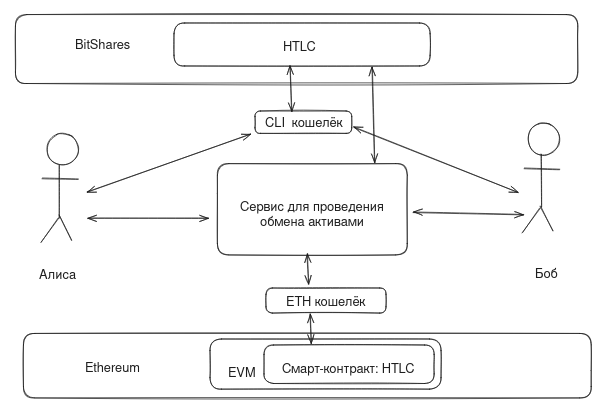
\includegraphics[scale=0.65]{res/architecture}
\caption{Структура сервиса}
\label{pic:architecture}
\end{figure}

На этой схеме изображёны участники обмена активами, Алиса и Боб, с и две изолированные блокчейн сети -- BitShares и Ethereum. Так же на схеме показаны два основных элемента, которые входят в наш сервис -- это смарт-контракт для сети Ethereum и веб-интерфейс сервиса, который обеспечивает безопасный обмен.

В верхней части диаграммы находится платформа BitShares, где HTLC реализован как часть узла блокчейна. Алиса и Боб взаимодействуют с BitShares через CLI кошелёк, который служит интерфейсом для выполнения операций. С этого кошелька уходят подписанные операции в сеть BitShares. Из соображений безопасности, мы не стали хранить приватный ключ пользователя в сервисе. Это, очевидно, снижает удобство всей операции, но тут мы сталкиваемся с классической проблемой выбора между удобством и безопасностью.

Сервис для проведения обмена активами генерирует команды для CLI кошелька на стороне BitShares, и готовит транзакции на подписание любым ETH кошельком на стороне Ethereum. Этот сервис получает команды от Алисы и Боба, обрабатывает их и отслеживает состояние контрактов в обеих блокчейнах.

На стороне Ethereum изображён EVM (Ethereum Virtual Machine) и смарт-контракт HTLC, который аналогично HTLC на BitShares обеспечивает процесс обмена активами без доверия. Обе стороны сделки имеют возможность провести валидацию содержимого блокчейна, чтобы удостовериться что он выполняет ровно то, что заявлено..

Сам сервис, CLI кошелёк для BitShares и ETH кошелёк для Ethereum изображены в одном экземпляре, но это сделано только чтобы не загромождать схему. На самом деле, каждый пользователь пользуется своим экземпляром.

Диаграмма иллюстрирует, как Алиса и Боб, используя свои кошельки и взаимодействуя через сервис для проведения обмена активами, могут безопасно обмениваться активами между двумя различными блокчейн-платформами, BitShares и Ethereum, с использованием механизма HTLC для обеспечения безопасности и надежности процесса.

\subsection{Алгоритм работы сервиса}

Упрощенный алгоритм работы сервиса представлен на диаграмме последовательности на рис. \ref{pic:sequence}. В декомпозиции этого процесса сложность представляет определение границ каждой сущности, чтобы привести работу обоих блокчейнов к единой точке отсчёта.

\begin{figure}[H]
\centering
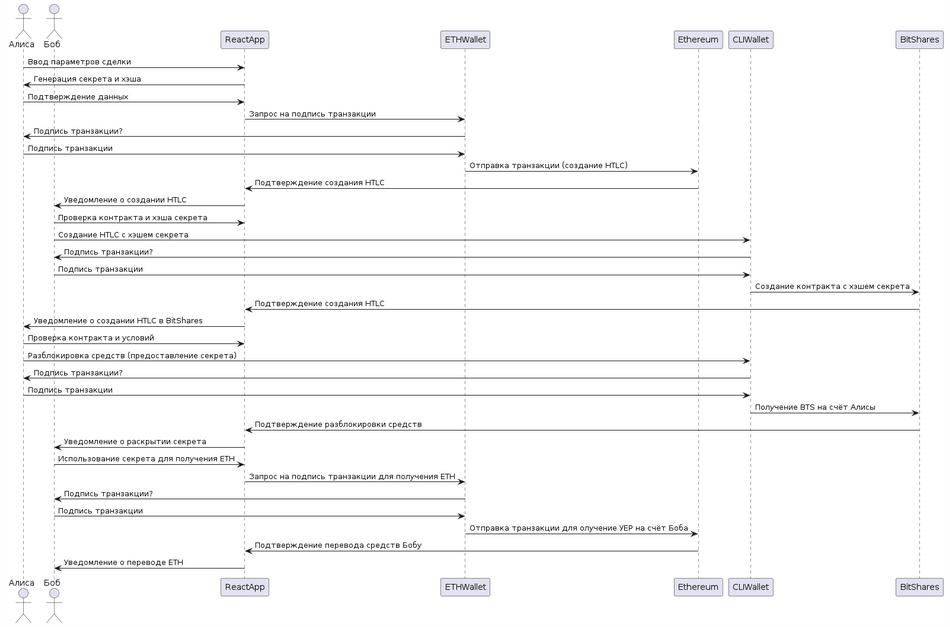
\includegraphics[scale=0.5]{res/sequence}
\caption{Алгоритм работы сервиса на диаграмме последовательности}
\label{pic:sequence}
\end{figure}

Алиса и Боб договорились провести обмен активами: Алиса отдаёт свои ETH, а в ответ получает BTS от Боба. Первым шагом Алиса запускает наше React приложение, где она вводит параметры предстоящей сделки. В интерфейсе она указывает максимальное время исполнения заявки, сумму ETH для обмена и адрес получателя, которым будет Боб. Кроме того, приложение генерирует уникальный секрет и вычисляет его хэш, который затем используется в транзакции. После подготовки всех данных приложение вызывает Enkrypt (MyEtherWallet) для подписания этой транзакции. Алиса подписывает и отправляет транзакцию в сеть Ethereum, где создаётся HTLC контракт.

Когда транзакция проходит в Ethereum, Боб получает уведомление о появлении нового HTLC контракта. Он проверяет, что контракт создан на его адрес, и сверяет хэш секрета. После этого Боб создаёт аналогичный HTLC контракт в сети BitShares с помощью CLI-кошелька. В этом контракте получателем указывается адрес Алисы, а хэш совпадает с тем, что он увидел в сети Ethereum. Существенной особенностью процесса является то, что время жизни контракта в BitShares должно быть меньше, чем в Ethereum, чтобы минимизировать риски для Боба. Если Алиса не сможет предоставить секрет вовремя, Боб сможет вернуть свои BTS.

После создания контракта в сети BitShares, Алиса получает уведомление и проверяет условия контракта, включая количество BTS и параметры хэш-замка. Убедившись в правильности всех условий, Алиса использует свой CLI-кошелёк, чтобы предоставить секрет и получить свои BTS. Поскольку контракт был создан с использованием известного хэша секрета, Алиса легко разблокирует средства и забирает их.

Как только Боб видит, что секрет был раскрыт в сети BitShares, он использует этот же секрет для получения своих ETH из контракта в сети Ethereum. Сервис помогает ему подготовить соответствующую транзакцию, и Боб подписывает её с помощью Enkrypt (MyEtherWallet). Остальные пользователи могут видеть раскрытый секрет, но ничего не могут сделать с активами, так как контракт чётко определяет, что только Боб может забрать ETH.

Сервис обеспечивает безопасный обмен активами между изолированными распределёнными реестрами с использованием механизма атомарных свопов через HTLC. Реализация на React обеспечивает удобный интерфейс для взаимодействия пользователей с блокчейнами, а использование Enkrypt (MyEtherWallet) и CLI BitShares позволяет надёжно подписывать и отправлять транзакции. Этот подход позволяет избежать необходимости доверия между сторонами и минимизирует риски благодаря использованию проверенных криптографических методов и смарт-контрактов.

\section{Программная реализация прототипа}

\subsection{Сервис обмена}

Сервис обмена представляет собой графическое приложение на React. Приложение упаковано в Docker, это значит что любая сторона может запустить экземпляр приложения независимо друг от друга. Но даже если будет использоваться один веб-сервер для раздачи JS-файлов, они всё равно могут быть проверены сторонами перед исполнением.

Для взаимодействия с Ethereum, используется универсальное API, которое позволяет подписывать транзакции в отдельном окне. BitShares не имеет интеграции с такими средствами, а хранить приватный ключ в браузере мы сочли недостаточно надёжным. Поэтому для BitShares мы даём команды, которые пользователь может выполнить в cli-интерфейсе.

Листинг \ref{lst:app} представляет собой исходный код основной формы React-приложения для реализации интерфейса для атомарного свопа между Ethereum (ETH) и BitShares (BTS).

\lstinputlisting[language=JavaScript, caption={React приложение атомарного свапа}, captionpos=t, label=lst:app]
{res/App.js}

В данном коде, начиная с первой строки, происходит импорт необходимых зависимостей из библиотек \textit{react} и \textit{styled-components}, а также компонентов из локальных файлов (строки 1-5). Далее создается стилизованный компонент \textit{Container}, который устанавливает базовые стили для всего приложения, такие как цвет фона, минимальная высота и параметры выравнивания (строки 8-16). Компонент \textit{Header} стилизует заголовок, задавая ему цвет и отступы (строки 18-21).

Затем определяется контейнер для вкладок (\textit{TabContainer}), который используется для выравнивания элементов вкладок (строки 23-26). Сами вкладки (\textit{Tab}) стилизованы с учетом состояния \textit{active}, определяющего их фон и другие параметры стиля, такие как отступы, границы и эффекты при наведении (строки 28-41). Компонент \textit{Content} задает стили для основного содержимого, включая белый фон, отступы, скругленные углы и тень (строки 43-49).

Функция \textit{App} представляет собой основной функциональный компонент приложения. В нем используется хук \textit{useState} для управления активной вкладкой, которая по умолчанию установлена на \textit{'eth'} (строка 53). Если в браузере пользователя не установлен MetaMask, выводится предупреждение и выполнение функции прекращается (строки 45-58). Определяются провайдер Ethereum и адрес контракта, а также провайдер BitShares (строка 62).

Основной JSX-возврат начинается с рендеринга контейнера \textit{Container}, в который вложены заголовок (\textit{Header}), контейнер вкладок (\textit{TabContainer}) и основной блок содержимого (\textit{Content}) (строки 65-96). В \textit{TabContainer} размещаются две вкладки, одна для Ethereum, другая для BitShares, при клике на которые активная вкладка изменяется с помощью функции \textit{setActiveTab} (строки 79-94). 

Содержимое блока \textit{Content} меняется в зависимости от активной вкладки. Если активна вкладка \textit{eth}, отображаются компоненты \textit{InitiateSwap}, \textit{Withdraw}, \textit{CheckStatus} и \textit{Refund}, которым передаются необходимые параметры (строки 73-78). Если активна вкладка \textit{bts}, показывается статический контент с инструкциями для BitShares и компонент \textit{CheckStatus} (строки 81-93).

В конце файл экспортирует компонент \textit{App} по умолчанию, чтобы его можно было использовать в других частях приложения (строка 100).

Рассмотрим ещё один пример кода -- компонент инициализации HTLC в листинге \ref{lst:InitiateSwap}.

\lstinputlisting[language=JavaScript, caption={Фукциональный React-компонент инициализации атомарного свапа}, captionpos=t, label=lst:InitiateSwap]
{res/InitiateSwap.js}

В этом коде сначала импортируются необходимые зависимости из библиотек \textit{react} и \textit{styled-components}, а также модуль \textit{ethers} из библиотеки \textit{ethers.js} для работы с Ethereum (строки 1-3). Затем определяются стили для компонента \textit{input} в объекте \textit{styles}, который включает отступы, размер шрифта, скругленные углы и границу (строки 5-12).

Создается стилизованный компонент \textit{Form}, который представляет собой контейнер для формы, выстраивающий свои элементы в колонку с промежутком в 10 пикселей (строки 15-19). Компонент \textit{Input} стилизует поля ввода, добавляя отступы, границу и скругленные углы (строки 21-25). Кнопка \textit{Button} имеет стили для фона, цвета текста, отступов, скругленных углов и эффекта при наведении (строки 27-38). Компонент \textit{Message} отображает сообщение, изменяя его цвет в зависимости от свойства \textit{error} (строки 40-43).

Компонент \textit{InitiateSwap} является функциональным компонентом, который принимает параметры \textit{ethContractAddress}, \textit{ethProvider} и \textit{btsProvider} (строка 45). Внутри него используются хуки \textit{useState} для управления состоянием различных полей формы, таких как получатель ETH, сумма ETH, секрет, время блокировки и сообщение, а также для проверки валидности адреса получателя (строки 46-51).

Функция \textit{generateSecret} создает новый секрет с помощью \textit{ethers.hexlify} и \textit{ethers.randomBytes}, и устанавливает его в состоянии компонента (строки 53-61). Функция \textit{validateRecipient} проверяет валидность Ethereum-адреса с помощью \textit{ethers.isAddress} (строки 58-61). В функции \textit{handleRecipientChange} обрабатывается изменение адреса получателя, обновляя состояние и проверяя валидность адреса (строки 63-67).

Основная функция \textit{initiateSwap} выполняет процесс инициирования свопа. Она запрашивает аккаунты у пользователя, создаёт контракт, инициирует своп, обрабатывает транзакцию и отображает сообщение о результате (строки 69-90). 

JSX-возврат компонента \textit{InitiateSwap} включает форму с заголовком и полями ввода для получателя ETH, суммы ETH, секрета и времени блокировки, а также кнопки для генерации секрета и инициирования свопа. Поле ввода для получателя ETH динамически меняет стили в зависимости от его валидности (строки 92-130).

Компонент \textit{InitiateSwap} экспортируется по умолчанию для использования в других частях приложения (строка 132).

Проект состоит из множества других компонентов и служебных файлов (Dockerfile, docker-compose.yml), но их подробное рассмотрение нецелесообразно.

С точки зрения анализа лучших практик, можно отметить предупреждения от системы сборки React-проекта об устаревании некоторых пакетов, которые используются в качестве зависимости. Это не является критической проблемой, т.к. сервис может работать локально и не имеет доступа к приватным ключам пользователя. С точки зрения UI/UX можно поработать над более наглядным интерфейсом, добавлением динамики при обработке транзакции узлами блокчейнов и сделать более подробные инструкции для BitShares части проекта. Но эти исследования достаточно ресурсоёмки, и останутся за пределами данной работы.

\subsection{Интеграция блокчейна с виртуальной машиной (Ethereum)}

\subsubsection{Смарт-контракт для блокчейна Ethereum}

Для исполнения HTLC в блокчейне Ethereum был подготовлен специальный смарт-контракт на языке Solidity (см. листинг \ref{lst:solidity}). Этот смарт-контракт реализует механизм атомарных свапов (Atomic Swap) с использованием Hash Time-Locked Contracts (HTLC) на языке Solidity.

\lstinputlisting[language=Solidity, caption={Фрагмент исходного кода модифицированного файла игры}, captionpos=t, label=lst:solidity]
{res/HTLC.sol}

\subsubsection{Описание смарт-контракта и анализ лучших практик}

Рассмотрим содержимое этого смарт-контракта:

В строках 1-2 объявлена лицензия MIT. Это разрешающая лицензия, которая позволяет использовать, модифицировать и распространять код при условии сохранения оригинального уведомления о лицензии. Так же указана версия компилятора Solidity 0.8.0.
   
В строке 20 начинается объявление смарт-контракта под названием \textit{AtomicSwap}, который реализует хешированные контракты с временной блокировкой для обмена ETH.

В строке 22 объявлена структура \textit{Swap}, которая содержит информацию о каждом обмене. Структура включает поля: 
\begin{itemize}
\item отправитель;
\item получатель;
\item сумма перевода;
\item хеш секретного ключа;
\item срок блокировки;
\item флаги состояния исполнения и возврата средств;
\item сам секретный ключ (пока ключ не раскрыт, это поле будет пустым).
\end{itemize}

В строке 34 объявлено хранилище \textit{swaps}, представляющее собой отображение идентификатора свопа (\textit{bytes32}) на структуру \textit{Swap}. Это позволяет сохранять и получать данные о каждом свопе по его уникальному идентификатору.

В строках 37-49 объявлены события \textit{SwapInitiated}, \textit{Withdraw} и \textit{Refund}, которые логируют важные действия в контракте: создание нового свопа, вывод средств и возврат средств соответственно.

В строках 60-97 реализована функция \textit{initiateSwap}, которая создаёт новый своп. Эта функция принимает адрес получателя, хеш секретного ключа и срок блокировки, а также сумму ETH через \textit{msg.value}. В функции проверяются условия корректности входных данных и создаётся уникальный идентификатор свопа. Затем данные свопа сохраняются в хранилище, и генерируется событие \textit{SwapInitiated}.

В строках 105-121 реализована функция \textit{withdraw}, которая позволяет получателю вывести ETH, зная секретный ключ. Функция проверяет корректность свопа, соответствие хеша секретного ключа, текущее время и статус свопа. Если все условия выполнены, средства переводятся на адрес получателя, и генерируется событие \textit{Withdraw}.

В строках 128-140 реализована функция \textit{refund}, которая позволяет отправителю вернуть свои средства после истечения срока блокировки. Функция проверяет существование свопа, права отправителя, срок блокировки и статус возврата. При выполнении условий средства возвращаются отправителю, и генерируется событие \textit{Refund}.

В строках 148-150 реализована функция \textit{getSecretHash}, которая позволяет получить хеш секретного ключа для указанного свопа. Эта функция публичная и предназначена для получения информации о свопе.

В строках 158-161 реализована функция \textit{getSecret}, которая позволяет получить секретный ключ для указанного свопа после его успешного завершения (вывода средств). Эта функция также публичная, но доступ к секрету возможен только после успешного завершения свопа.

С точки зрения следования лучшим практикам, использование \textit{block.timestamp} может быть ненадежным, так как майнеры могут слегка манипулировать этим значением. Хотя это не является критическим для нашего случая, это требование может варьироваться в зависимости от потребностей и сценариев использования. Текущая реализация позволяет только получателю снять средства или инициатору вернуть их после истечения временного замка. В некоторых случаях может быть полезно предусмотреть возможность для инициатора свапа отозвать средства до истечения временного замка, если это необходимо. Контракт не допускает повторную инициацию свапа с тем же \textit{\_swapId}. Теоретически существует вероятность, что в следствии коллизии разные входные данные могут дать одно и тоже значение на выходе в следствии коллизии хэш-функции. Переменные состояния, такие как \textit{withdrawn} и \textit{refunded}, могут быть объединены в один байт с битовыми флагами, что уменьшит потребление газа, но сделает код менее читаемым.

Представленный смарт-контракт полностью справляется с задачей обеспечения безопасного выполнение атомарных свапов. Использованием временных замков и хешей секретных ключей надёжно защищает интересы сторон обмена.

\subsubsection{Процесс выполнения смарт-контракта}

Виртуальная машина Ethereum (EVM) представляет собой децентрализованную вычислительную платформу, на которой выполняются смарт-контракты, написанные на языке программирования Solidity. Когда смарт-контракт, такой как описанный выше, загружается в блокчейн Ethereum, он компилируется в байт-код, который может быть интерпретирован и выполнен EVM.

Процесс выполнения смарт-контракта EVM начинается с транзакции, инициированной пользователем или другим контрактом. Транзакция включает данные, такие как адрес контракта, который будет вызван, и передаваемые параметры. В случае представленного выше смарт-контракта, первая транзакция может быть вызовом функции \textit{initiateSwap}, которая инициализирует новый своп.

Когда транзакция достигает узла в сети Ethereum, узел передает транзакцию EVM для обработки. EVM создает изолированное окружение для выполнения кода контракта, обеспечивая, что каждое выполнение является детерминированным и не зависит от состояния других контрактов. Это окружение включает стек, область памяти и область хранения, которые используются для управления данными и состоянием контракта.

EVM начинает выполнение байт-кода контракта, интерпретируя каждую инструкцию последовательно. В функции \textit{initiateSwap}, EVM выполняет проверки условий, таких как корректность адреса получателя и положительное значение \textit{msg.value}, чтобы убедиться в валидности данных. Затем EVM генерирует уникальный идентификатор свопа, используя хеширование, и сохраняет данные свопа в области хранения контракта. После успешного выполнения этих операций, EVM создает лог-событие \textit{SwapInitiated}, записывая его в журнал транзакций, что позволяет участникам сети отслеживать произошедшие изменения.

Аналогичным образом, при вызове функции \textit{withdraw} или \textit{refund}, EVM выполняет последовательность инструкций, соответствующих этим функциям. Для \textit{withdraw}, EVM проверяет, что секретный ключ соответствует хешу и что срок блокировки не истек. Если все условия выполняются, средства переводятся получателю, и статус свопа обновляется. В случае \textit{refund}, EVM проверяет, что срок блокировки истек и что своп не был уже возвращен, после чего средства возвращаются отправителю.

Каждая из этих операций требует вычислительных ресурсов, и каждая инструкция байт-кода имеет стоимость в газе, который является единицей измерения затрат на вычисления в сети Ethereum. Пользователи, инициирующие транзакции, платят за газ, чтобы компенсировать узлы, выполняющие вычисления.

В процессе выполнения этих функций, EVM обеспечивает соблюдение всех условий и инвариантов контракта, используя свой механизм консенсуса и проверки транзакций. Любые изменения состояния контракта фиксируются в блокчейне, делая их необратимыми и прозрачными. События, генерируемые контрактом, позволяют отслеживать все действия, связанные с свапами, что повышает прозрачность и доверие к контракту.

\subsection{Интеграция блокчейна без виртуальной машины (BitShares)}

Для работы с HTLC в BitShares используется несколько ключевых API. Для их вызова можно использовать библиотеку на JavaScript, но это создаёт проблему хранения приватного ключа пользователя. В качестве альтернативы, можно использовать CLI-интерфейс. В этом случае проблема защиты приватного ключа полностью остаётся на стороне пользователя. Рассмотрим назначение основных API, более подробное значение всех параметров можно найти в документации проекта \cite{label61}.

\begin{itemize}
\item htlc\_create\\
Создает HTLC контракт, который блокирует указанное количество активов до выполнения условий.
\item htlc\_redeem\\
Погашает HTLC контракт, передавая средства получателю при предъявлении правильного секрета.
\item get\_htlc\\
Получает информацию о конкретном HTLC контракте по его ID.
\item get\_htlc\_by\_from\\
Получает список HTLC контрактов, созданных указанным аккаунтом.
\item get\_htlc\_by\_to\\
Получает список HTLC контрактов, где указанный аккаунт является получателем.
\item htlc\_extend\\
Расширяет время истечения HTLC контракта.
\end{itemize}

Эти команды предоставляют основные функции для работы с HTLC контрактами в блокчейне BitShares, включая создание, погашение, проверку и расширение времени истечения контрактов.

BitShares работает со смарт-контрактами внутри ноды, предоставляя функциональность, аналогичную смарт-контрактам в Ethereum, но с некоторыми ключевыми отличиями. Основная идея состоит в том, что операции, подобные HTLC (Hashed TimeLock Contract), выполняются непосредственно в узле (ноде) BitShares, обеспечивая высокую производительность и надежность.

В BitShares смарт-контракты реализуются в виде встроенных операций, которые выполняются на уровне блокчейна, что имеет свои особенности

\begin{enumerate}
\item Встроенные операции.\\
В BitShares есть ряд предопределенных операций, которые выполняют определенные функции. HTLC – одна из таких операций. Эти операции выполняются непосредственно в блокчейне и обрабатываются нодами сети.
\item Высокая производительность.\\
Поскольку операции предопределены и выполняются непосредственно в нодах, BitShares может обрабатывать транзакции очень быстро и эффективно. Это контрастирует с Ethereum, где каждый смарт-контракт исполняется виртуальной машиной (EVM), что может быть медленнее и требует больше ресурсов.
\item Меньшая гибкость.\\
Хотя предопределенные операции обеспечивают высокую производительность, они менее гибки, чем пользовательские смарт-контракты в Ethereum. В BitShares нельзя создать произвольный смарт-контракт с любой логикой; можно использовать только те операции, которые уже реализованы в системе.
\end{enumerate}

Можно видеть, подход BitShares к построению сети и выполнению операций сильно отличается от подхода Ethereum. Однако использование атомарных свапов позволяет эффективно проводить обмен даже между столь различными проектами.

\section{Тестирование системы}

В данном разделе рассмотрим модульное и системное тестирование.

\subsection{Модульное тестирование}

Для проверки корректной работы сервиса код был покрыт unit­ тестами. Сервис имеет большое количество внешних зависимостей, которые по возможности были мокированы. Пример тестирования компонента инициализации атомарного свапа представлен в листинге \ref{lst:InitiateSwapTest}.

\lstinputlisting[language=JavaScript, caption={Unit-тестирование компонента инициализации атомарного свапа}, captionpos=t, label=lst:InitiateSwapTest]
{res/InitiateSwap.test.js}

Рассмотрим содержимое тестового сценария.

В строках 1-4 импортируются необходимые библиотеки, тестируемый компонент \textit{InitiateSwap}, и добавляется библиотека \textit{ethers}.

В строке 7 используется метод \textit{jest.mock} для мока библиотеки \textit{ethers}, что позволяет изолировать тесты от реальной реализации.

В строках 9-42 начинается описание тестовой группы \textit{describe}, включающей несколько тестов для компонента \textit{InitiateSwap}. В строках 11-18 задаются моковые данные для пропсов компонента, такие как \textit{mockEthContractAddress}, \textit{mockEthProvider} и \textit{mockBtsProvider}.

В строках 20-23 используется метод \textit{beforeEach} для очистки всех моков перед каждым тестом, чтобы избежать влияния предыдущих тестов на текущий.

Тест в строках 25-42 проверяет корректность рендеринга элементов формы. Сначала рендерится компонент с моковыми пропсами. Затем с помощью различных методов \textit{screen} проверяется наличие всех ожидаемых элементов формы: заголовка, полей ввода для ETH, Secret и Timelock, а также кнопок "Generate Secret" и "Initiate Swap".

Тест в строках 44-63 проверяет корректность обновления полей ввода. После рендеринга компонента находим поле ввода ETH, симулируем ввод значения "1.5" и проверяем, что значение обновилось корректно.

Тест в строках 65-89 проверяет функцию \textit{initiateSwap} компонента. Здесь используются моки для метода \textit{ethers.parseEther}. Компонент рендерится, заполняет необходимые поля ввода и симулирует клик по кнопке "Initiate Swap". Проверяется, что вызов метода \textit{initiateSwap} не происходит, поскольку управление должно перехватить кошелёк.

Тест в строках 91-129 проверяет валидность адреса Ethereum. Поле ввода заполняется невалидным адресом, и проверяется, что граница поля ввода меняется на красный цвет. Затем поле заполняется валидным адресом (с использованием мока \textit{ethers.isAddress}), и проверяется, что граница поля ввода меняется на зеленый цвет.

Вывод консоли после запуска тестов после запуска юнит тестов показан на рис. \ref{pic:InitiateSwapTestConsole}.

\begin{figure}[H]
\centering
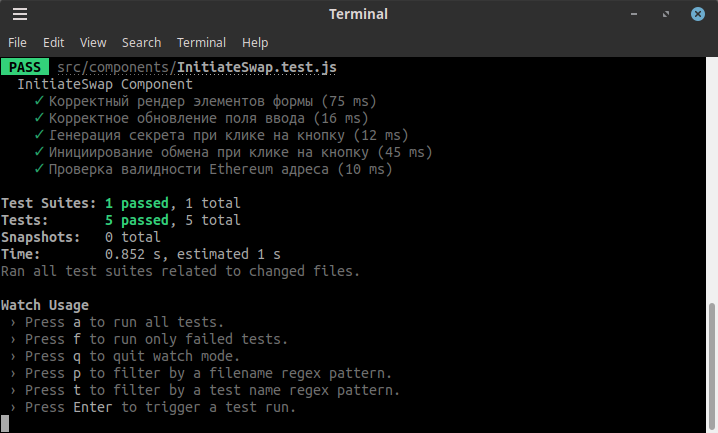
\includegraphics[scale=0.65]{res/console-out}
\caption{Вывод консоли после запуска тестов}
\label{pic:InitiateSwapTestConsole}
\end{figure}

Представленные тесты обеспечивают частичную проверку некоторых функций компонента \textit{InitiateSwap}, включая рендеринг, обработку пользовательского ввода и взаимодействие с внешними библиотеками. В действительности для тестирования сервиса было разработано множество тестов, но приводить их все в данном отчёте не целесообразно.

\subsection{Системное тестирование}

Системное тестирование связано с рядом сложностей, основная из которых это подготовка тестового окружения.

\subsubsection{Разворачивание тестовой сети Ethereum}

Для локальной разработки и тестирования Ethereum широко используется фреймворк Ganache. Это инструмент для запуска сети Ethereum на тестовом стенде, который позволяет разработчикам создавать, тестировать и развертывать смарт-контракты в безопасной и контролируемой среде. Ganache обладает полезными качествами, необходимыми разработчику:

\begin{enumerate}

\item Локальная сеть Ethereum.\\
Ganache запускает локальную версию сети Ethereum, позволяя вам разворачивать и тестировать смарт-контракты без необходимости взаимодействия с основной сетью (mainnet) или тестовыми сетями (testnet).

\item Контроль над сетью.\\
Разработчик может контролировать параметры сети, такие как число генерируемых блоков, сложность майнинга, учетные записи и их баланс. Это позволяет моделировать различные сценарии и тестировать поведение смарт-контрактов в разных условиях.

\item Легкий доступ к аккаунтам.\\
Ganache предоставляет готовые учетные записи с предустановленным балансом ETH, что упрощает процесс разработки и тестирования.

\item UI интерфейс и командная строка.\\
Ganache доступен как в виде графического интерфейса (Ganache UI), так и в виде утилиты командной строки (Ganache CLI), что позволяет выбрать наиболее удобный способ работы.

\end{enumerate}

Можно произвести запуск Ganache в Docker контейнере, для этого используем следующую команду для запуска:

\begin{lstlisting}[style=CommandLineStyle, belowskip=-2 \baselineskip]
$ docker run -d -p 8545:8545 --name ganache trufflesuite/ganache --accounts 10 --defaultBalanceEther 100
\end{lstlisting}
\vspace{-10pt}

Этой командой мы запутили тестовую сеть Ethereum, которая доступна на порту 8545, а так же создали 10 аккаунтов, с балансом в 10 монет у каждого.

Чтобы увидеть аккаунты, их баланс и другие параметры сети можно выполнить следующую команду 

\begin{lstlisting}[style=CommandLineStyle, belowskip=-2 \baselineskip]
$ docker logs ganache
\end{lstlisting}

Примерый вывод этой команды представлен в листинге \ref{lst:ganachelog}. 

\lstinputlisting[language={}, caption={Список доступных аккаунтов в тестовой сети Ethereum}, captionpos=t, label=lst:ganachelog]
{res/ganachelog.txt}

Теперь мы можем развертывать и тестировать смарт-контракты в локальной сети Ethereum, запущенной с помощью Ganache.

\subsubsection{Деплой смарт-контракта в тествую сеть Ethereum}

Для подулючения к тестовой сети можно использовать Truffle или сразу Web3.js.

Новый проект миграции можно подготовить командой

\begin{lstlisting}[style=CommandLineStyle, belowskip=-2 \baselineskip]
$ truffle init
\end{lstlisting}

Сприпт миграции представлен в листинге \ref{lst:TruffleDeploy}. Он полагается на то, что файл смарт-контра доступен по пути \textit{contracts\\HTLCContract.sol}.

\lstinputlisting[language=JavaScript, caption={Скрипт миграции Truffle}, captionpos=t, label=lst:TruffleDeploy]
{res/contract_deploy.js}

Для подключения к тестовой сети, нужно указать её адрес и порт, как это показано в листинге  \ref{lst:TruffleConnect}. Там же показан и выбор версии компилятора Splidity.

\lstinputlisting[language=JavaScript, caption={Подключение к тестовой сети}, captionpos=t, label=lst:TruffleConnect]
{res/truffle-config.js}

Провести развёртывание контракта можно командной
\begin{lstlisting}[style=CommandLineStyle, belowskip=-2 \baselineskip]
$ truffle migrate
\end{lstlisting}

Эта команда скомпилирует смарт-контракт и развернет его на указанной в конфигурации сети. Теперь смарт-контракт развернут на Ganache и готов к тестированию и дальнейшему взаимодействию.

\subsubsection{Разворачивание тестовой сети BitShares}

Подготовка и запуск тестовой сети Bitshares так же возможна через Docker. Для этого можно выполнить следующую команду

\begin{lstlisting}[style=CommandLineStyle, belowskip=-2 \baselineskip]
$ docker run -d -p 8090:8090 -p 8091:8091 -v $(pwd)/bitshares_data:/bitshares/witness_node_data_dir --name bitshares-testnet bitshares/bitshares-core:latest
\end{lstlisting}

Эта команда создаст и запустит Docker контейнер в фоновом режиме. Порты 8090 и 8091 проброшены для доступа к PRC и P2З интерфейсам. Локальная директория bitshares\_data смонтирована в контейнер для хранения данных блокчейна.

После этого нужно подлкючиться к ноде используя CLI-кошелёк и выполнить следующие три команды

\begin{lstlisting}[style=CommandLineStyle, belowskip=-2 \baselineskip]
> import_key nathan "5KQwrPbwdL6PhXujxW37FSSQZ1JiwsST4cqQzDeyXtP79zkvFD3"
> import_balance nathan ["5KQwrPbwdL6PhXujxW37FSSQZ1JiwsST4cqQzDeyXtP79zkvFD3"] true
> upgrade_account nathan true
\end{lstlisting}

Первая команда позволяет импортировать приватный ключ пользователя nathan. Вторая команда инициирует перевод средств, заложенных в генезисе, на счёт пользователя, и далее он может распоряжаться этими средствами. Последняя команда переводит пользователя в расширенный режим, где ему открываются дополнительные возможности по управлению сетью.

\subsubsection{Проведение атомарного свопа в тестовых сетях}

Интерфейс сервиса осуществления атомарных свопов между Ethereum (ETH) и BitShares (BTS) представлен на рис. \ref{pic:ServiceInterface}. Сразу под заголовком находится выбор вкладок: одна отвечает за работу с  Ethereum, а другая вкладка для выбора BitShares.

\begin{figure}[H]
\centering
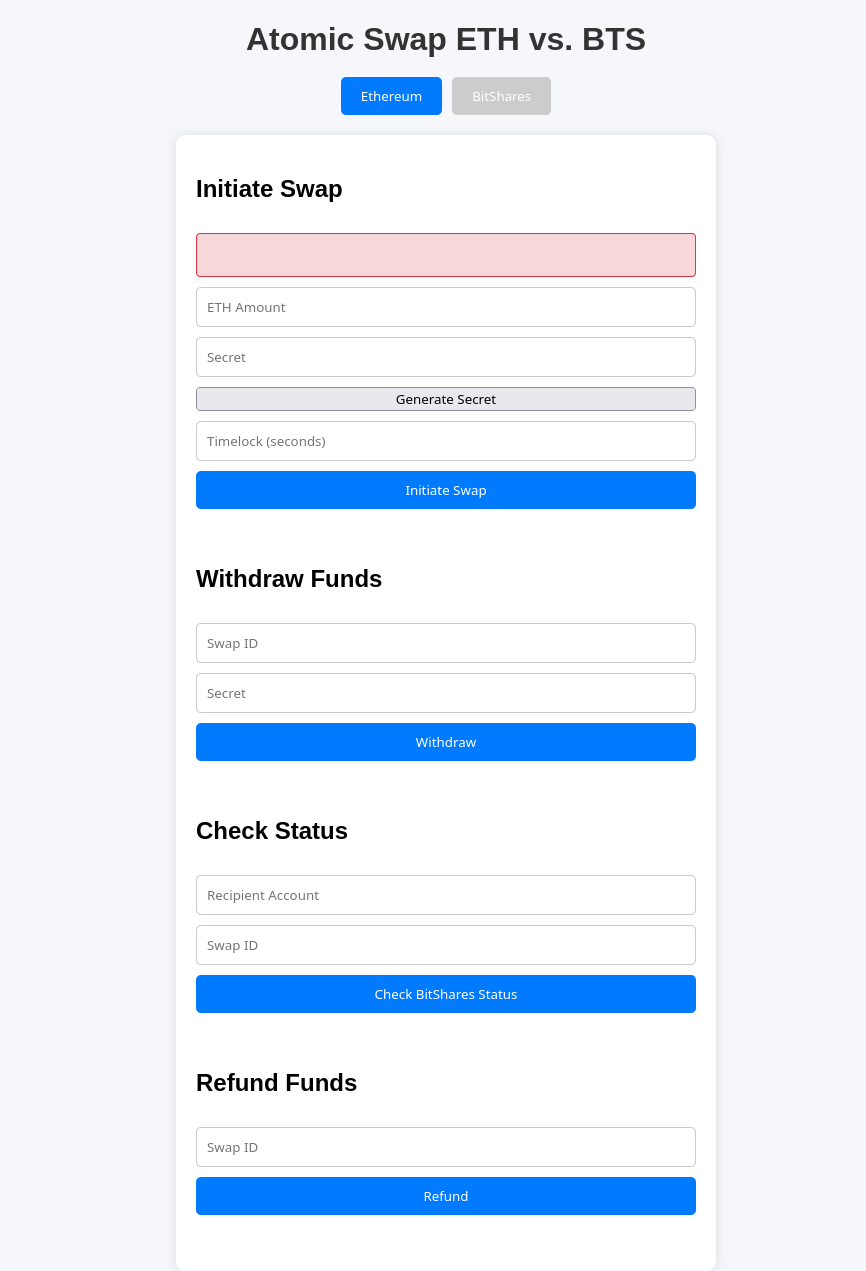
\includegraphics[scale=0.4]{res/ServiceInterface}
\caption{Пользовательский интерфейс сервиса обмена}
\label{pic:ServiceInterface}
\end{figure}

Основная часть интерфейса разделена на четыре секции:
\begin{itemize}
\item Первая секция называется "Initiate Swap". В этой секции пользователь может ввести сумму ETH, секрет, и время блокировки в секундах. Форма реагирует на ввод адреса получателя, проверяя что он является валидным адресом сети Ethernet. Адрес отправителя не нужен, т.к. он будет получен из подписи транзакции. Пользователь может самостоятельно задать секрет, либо сгенерировать его случайным образом. Для генерации случайного секрета предусмотрена отдельная серая кнопка "Generate Secret". Для завершения процесса инициации свопа имеется синяя кнопка "Initiate Swap".

\item Вторая секция называется "Withdraw Funds". Здесь пользователь может ввести идентификатор свопа (Swap ID) и секрет, после чего нажать синюю кнопку "Withdraw" для вывода средств на свой кошелёк. Как и в прошлом случае, адрес кошелька нам не нужен, мы получим его из подписи.

\item Третья секция, "Check Status", позволяет пользователю проверить статус свопа в сети BitShares. Для этого необходимо ввести учетную запись получателя и идентификатор свопа, а затем нажать синюю кнопку "Check BitShares Status". В данном случае, у нас нет возможности получить что либо из подписи, т.к. речь идёт о совершенно другом блокчейне, со своими структурами данных.

\item Четвертая и последняя секция называется "Refund Funds". В этой секции пользователь может ввести идентификатор свопа и нажать синюю кнопку "Refund" для возврата средств. Средства будут возвращены в случае, если они не были востребованы получателем, а срок действия контракта уже вышел. В случае с BitShares такой кнопки нет, т.к. там средства возвращаются отправителю автоматически.
\end{itemize}

Интерфейс предоставляет пользователю необходимый минимум инструментов для инициации атомарного свопа, вывода средств, проверки статуса транзакции и возврата средств в случае необходимости.

На рис. \ref{pic:ChromMetamask} изображен процесс подписания транзакции средствами MetaMask в браузере Chrome. Секция "Initiate Swap" заполнена тестовыми данными, и тут следует обратить внимание на поле с адесом получателя. Сервис воспринял строку "0xc0ffee254729296a45a3885639AC7E10F9d54979" как валидный ETH адрес, в результате поле ввода подкрашено зелёным цветом. Справа от основного интерфейса отображается всплывающее окно MetaMask. В этом окне заголовок "Connect with MetaMask" предлагает пользователю выбрать аккаунт для использования на данном сайте. Отображен аккаунт "Account 1 (0x5d7c3...eab8b)" с балансом 0 ETH. Этот аккаунт выбран для подключения, что отмечено галочкой. В верхней части этого окна виден адрес подключения http://127.0.0.1:3000, что говорит о тестовой сети.

\begin{figure}[H]
\centering
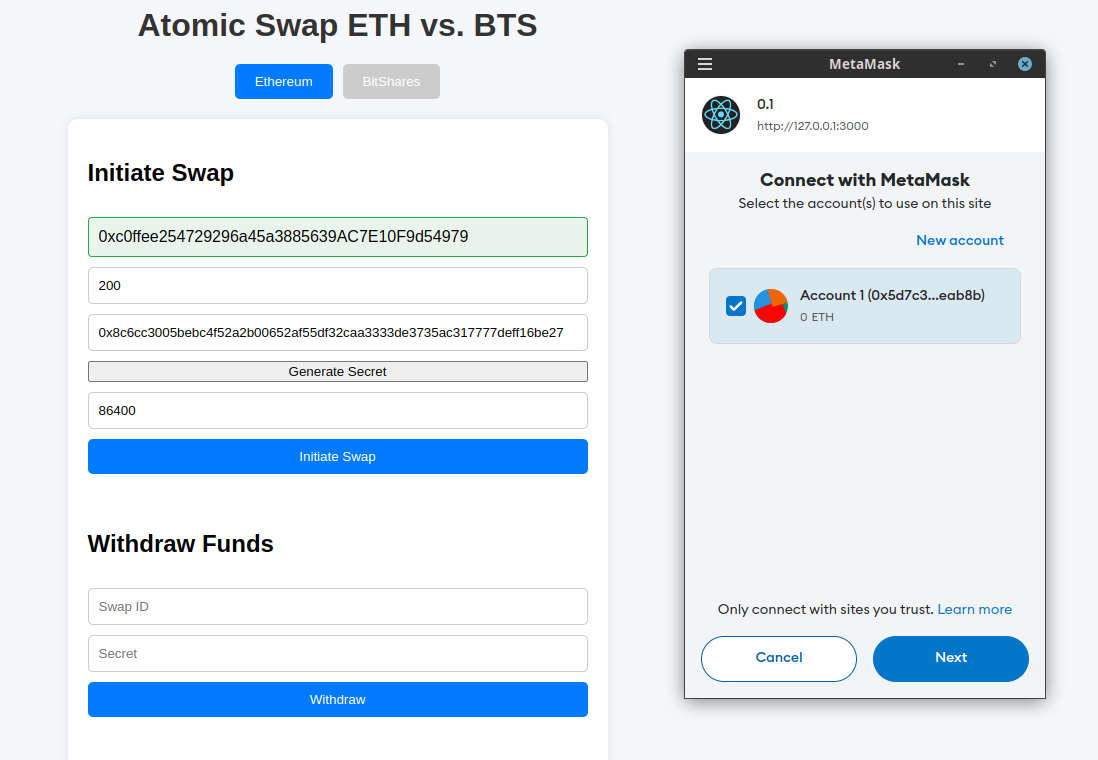
\includegraphics[scale=0.4]{res/ChromMetamask}
\caption{Браузер Chromium и криптокошелёк Metamask}
\label{pic:ChromMetamask}
\end{figure}

На рис. \ref{pic:FFEnkrtpt} так же изображен процесс подписания транзакции, только на этот раз используется браузер FireFox и окно авторизации Enkrypt (MyEtherWallet). Адрес получателя "0xc0ffee254729296a45a3885639AC7E10F9d54979" распознан как валидный, поэтому подсвечен зелёным. Интерфейс предупреждает пользователя, что его действия раскроют публичный адрес, баланс кошелька и активность для сети "127.0.0.1", которая является тестовой площадкой.

\begin{figure}[H]
\centering
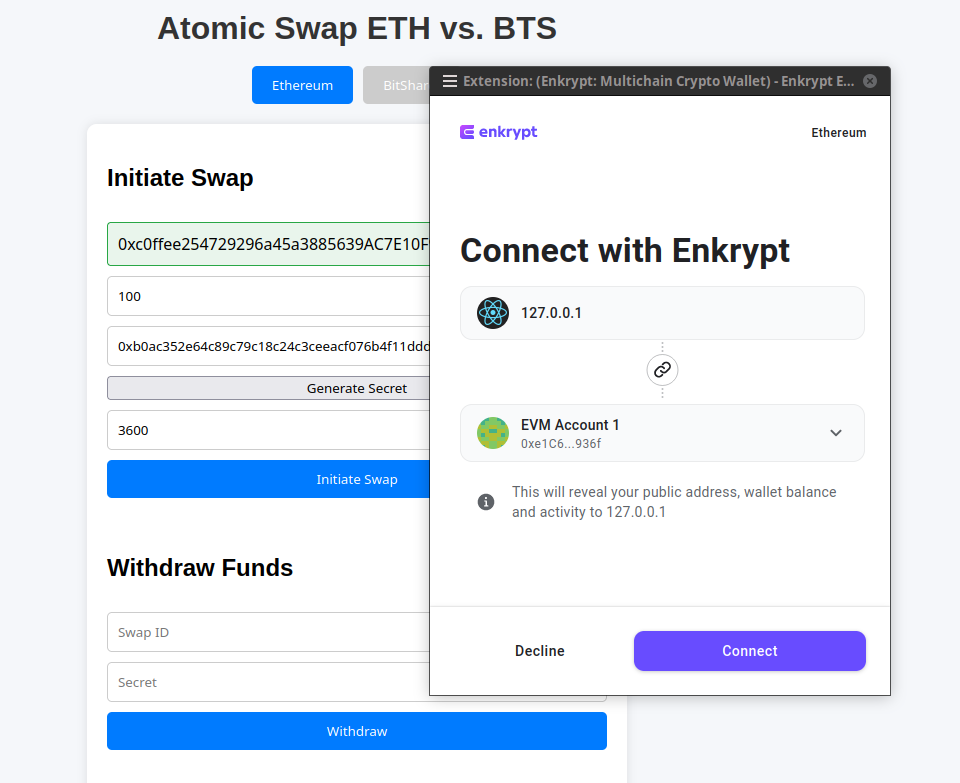
\includegraphics[scale=0.4]{res/FFEnkrtpt}
\caption{Браузер FireFix и криптокошелёк Enkrtpt (MyEtherWallet)}
\label{pic:FFEnkrtpt}
\end{figure}

Когда все контракты выполнены, баланс пользователя изменяется в криптокошельках. В этом контексте, криптокошельки не являются частью сервиса, поэтому их изображение тут не приводится. Сервис не знает баланс пользователя, хотя технически такую возможность реализовать можно.

Проводить операции с Ethereum достаточно просто. В случае с Bitshares, пользователю нужно использовать CLI-кошелёк и самостоятельно заботиться о безопасности своего приватного кошелька. Очевидно, это достаточно неудобно для конечных пользователей. Поддержки BitShares со стороны основных криптокошельков на данный момент нет, но это вполне можно реализовать внутри сервиса, если решить задачу надёжного хранения ключа.

Это может стать темой для дальнейших исследований.

\section{Выводы}

Исследование существующих подходов к межсетевому обмену, таких как использование доверительных сторон, мостов и пулов ликвидности, выявило ряд существенных недостатков. Метод атомарных свапов с использованием HTLC признан наиболее эффективным и безопасным решением для межсетевого обмена. Отсутствие централизованных элементов, гарантированная безопасность, фиксированная цена и возможность адаптации существующих блокчейнов делают этот подход оптимальным для построения сервиса обмена активами.

В этом разделе мы описали структуру сервиса, алгоритм его работы и выбор технологий для разработки. В качестве основного инструмента для построения пользовательского интерфейса был выбран React. Выбор Ethereum обусловлен наличием развитой инфраструктуры для создания и выполнения смарт-контрактов, а BitShares - высокой производительностью и низкими комиссиями за транзакции.

В разработке прототипа сервиса были решены следующие задачи:
\begin{itemize}
\item Создан веб-интерфейс на React, обеспечивающий удобное управление процессом обмена активами.
\item Разработан смарт-контракт для Ethereum, реализующий механизм HTLC.
\item Обеспечено взаимодействие сервиса с API блокчейна BitShares для управления HTLC-контрактами.
\end{itemize}

Представленное решение гарантирует полую децентрализация сервиса, исключающая необходимость доверия между сторонами сделки или к третьим сторонам.

В конце раздела, описывается процесс модульного и системного тестирования. Модульные тесты покрывают функциональность отдельных компонентов сервиса, а системное тестирование проводилось в тестовой сети Ethereum с использованием Ganache и в тестовой сети BitShares. Так же отмечены некоторые минусы, связанные с удобством пользователя, устранение которых может стать темой дальнейших исследований.

\chapter*{Заключение}
\addcontentsline{toc}{chapter}{Заключение}

В первом разделе данной работы проведено исследование технологии распределенных реестров, включая технологию блокчейн, как её частный случай. Проанализировано влияние DLT на различные отрасли, выделены её ключевые преимущества – безопасность, прозрачность и автоматизация. Особое внимание уделено проблеме интероперабельности блокчейн сетей, которая ограничивает взаимодействие между различными блокчейн платформами.

Во втором разделе рассмотрены существующие решения для обмена активами между блокчейнами, такие как централизованные биржи, атомарные свопы, мосты с использованием обернутых монет и пулов ликвидности, а также релейные блокчейны. Выявлены их сильные и слабые стороны, а также области применения. Отдельное внимание уделено вопросу доверия между сторонами. Проведено исследование возникновения этого доверия и возможные последствия для реальных проектов.

В последнем разделе была поставлена задача -- разработка сервиса для проведения обмена активами между изолированными распределенными реестрами без установления доверия. После анализа существующих подходов был сделан вывод, что механизм атомарных свопов с использованием HTLC является наиболее эффективным и безопасным.

Основные результаты работы:
\begin{itemize}
\item Разработан прототип сервиса обмена активами, использующий механизм атомарных свопов с HTLC. Сервис реализован с использованием React для создания пользовательского интерфейса, Ethereum для развертывания смарт-контрактов HTLC и BitShares для проведения обмена активами без использования виртуальной машины.

\item Проведено модульное тестирование разработанного сервиса, подтверждающее корректность работы отдельных компонентов.

\item Выполнено системное тестирование в тестовых сетях Ethereum (Ganache) и BitShares, демонстрирующее работоспособность сервиса в реальных условиях.
\end{itemize}

Возможные направления дальнейших исследований:
\begin{itemize}
\item Улучшение пользовательского интерфейса для упрощения взаимодействия с сервисом, особенно для пользователей BitShares и других блокчейн-проектов, не имеющих поддержки в популярных криптокошельках.

\item Интеграция с другими блокчейн платформами, расширяющая функциональность сервиса и увеличивающая количество доступных для обмена активов.

\item Исследование возможности реализации механизма HTLC для других популярных блокчейнов, таких как Bitcoin и Litecoin.

\item Разработка децентрализованного механизма хранения приватных ключей для повышения безопасности и удобства использования сервиса.
\end{itemize}

В заключение, разработанный прототип сервиса обмена активами демонстрирует потенциал механизма атомарных свопов с HTLC для решения проблемы интероперабельности блокчейн сетей. Дальнейшие исследования и разработки в этом направлении могут привести к созданию более совершенных и доступных инструментов для обмена активами между различными блокчейн платформами, способствуя развитию децентрализованных финансовых систем и укреплению доверия к блокчейн технологиям.
\begin{thebibliography}{00}
\addcontentsline{toc}{chapter}{Список использованных источников}

% https://www.overleaf.com/learn/latex/Bibliography_management_with_bibtex
% Use: \cite{label00}

\bibitem{label22} Аксаков А.Г., Свистунов А.Н., Бабич И.Н., Алтухов С.В., и др. Законопроект № 341257-8 О внесении изменений в отдельные законодательные акты Российской Федерации (в части установления экспериментальных правовых режимов в сфере цифровых инноваций на финансовом рынке) [Электронный ресурс], Система обеспечения законодательной деятельности. -- URL: https://sozd.duma.gov.ru/bill/341257-8 (дата обращения: 20.04.2024).

\bibitem{label29} Албычев А.С., Ильин Д.Ю. ВЫБОР СТЕКА ТЕХНОЛОГИЙ ВЫЧИСЛИТЕЛЬНОЙ ИНФРАСТРУКТУРЫ ДЛЯ ЭКСПЕРИМЕНТАЛЬНЫХ ИССЛЕДОВАНИЙ ЦИФРОВЫХ ВАЛЮТ // International Journal of Open Information Technologies. 2023. №4. URL: https://cyberleninka.ru/article/n/vybor-steka-tehnologiy-vychislitelnoy-infrastruktury-dlya-eksperimentalnyh-issledovaniy-tsifrovyh-valyut (дата обращения: 10.06.2024).

\bibitem{label23} Биржа Mt.Gox: крупнейший взлом в истории криптовалют [Электронный ресурс], ForkLog журнал о биткоине, технологии блокчейн и цифровой экономике. -- URL: https://forklog.com/cryptorium/birzha-mt-gox-krupnejshij-vzlom-v-istorii-kriptovalyut (дата обращения: 10.06.2024).

\bibitem{label15} Блокчейн в корпоративной архитектуре: дань моде или необходимость? [Электронный ресурс], Хабр. -- URL:  https://habr.com/ru/companies/web3\_tech/articles/658447/ (дата обращения: 01.04.2024).

\bibitem{label19} Болдачев А.В. Миф о консенсусе [Электронный ресурс], Издательство Открытые системы. -- URL:  https://www.osp.ru/os/2019/02/13054960 (дата обращения: 20.04.2024).

\bibitem{label25} Британская «дочка» Binance отказалась от регистрации в FCA [Электронный ресурс], ForkLog журнал о биткоине, технологии блокчейн и цифровой экономике. -- URL: https://forklog.com/news/britanskaya-dochka-binance-otkazalas-ot-registratsii-v-fca (дата обращения: 10.06.2024).

\bibitem{label30} Булыга Р.П., Сафонова И.В. Ерансформация методологии аудита в связи с использованием технологий блокчейн и DLT // Учет. Анализ. Аудит. 2021. №5. URL: https://cyberleninka.ru/article/n/transformatsiya-metodologii-audita-v-svyazi-s-ispolzovaniem-tehnologiy-blokcheyn-i-dlt (дата обращения: 10.06.2024).

\bibitem{label26} В Греции задержан россиянин, обвиняемый в отмывании \$4 млрд в биткоинах [Электронный ресурс], ForkLog журнал о биткоине, технологии блокчейн и цифровой экономике. -- URL: https://forklog.com/news/v-gretsii-zaderzhan-rossiyanin-obvinyaemyj-v-otmyvanii-4-mlrd-v-bitkoinah (дата обращения: 10.06.2024).

\bibitem{label1} Голосование по поправкам в Конституцию Российской Федерации [Электронный ресурс], Официальный сайт мэра Москвы. -- URL: https://www.mos.ru/city/projects/vote2020/\#rec168487887\#!/tab/207311641-4 (дата обращения: 01.04.2024).

\bibitem{label10} Егорова М.А., Белых В.С., Решетникова С.Б. Технология блокчейн: перспективы применения и значение для целей развития информационного общества // Юрист. 2019. N 7. С. 4-9.

\bibitem{label38} Использование технологии DLT на финансовых рынках поможет сэкономить \$100 млрд [Электронный ресурс], crypto.ru. -- URL: https://crypto.ru/ispolzovanie-dlt-pomozhet-sekonomit-100-mlrd/ (дата обращения: 20.04.2024).

\bibitem{label33} Моисеев А. Совершенствуем процедуру Know Your Customer с помощью блокчейна [Электронный ресурс], Лаборатория Касперского. -- URL: https://www.kaspersky.ru/blog/kyc-blockchain/27528/ (дата обращения: 20.04.2024).

\bibitem{label9} Нагродская В.Б. Новые технологии (блокчейн / искусственный интеллект) на службе права: научно-методическое пособие / под ред. Л.А. Новоселовой. М.: Проспект, 2019. 128 с.

\bibitem{label16} Программа льготного кредитования субъектов малого и среднего предпринимательства в 2019 – 2024 годах [Электронный ресурс], Государственная информационная система промышленности. -- URL: https://gisp.gov.ru/nmp/measure/9604994 (дата обращения: 01.04.2024).

\bibitem{label35} Полешкина И.О., Васильева Н.В. Технология Blockchain как инструмент управления цепями поставок с участием воздушного транспорта // Научный вестник МГТУ ГА. 2020. №2. URL: https://cyberleninka.ru/article/n/tehnologiya-blockchain-kak-instrument-upravleniya-tsepyami-postavok-s-uchastiem-vozdushnogo-transporta (дата обращения: 20.04.2024).

\bibitem{label24} Регулятор: QuadrigaCX обанкротилась из-за мошенничества ее основателя [Электронный ресурс], ForkLog журнал о биткоине, технологии блокчейн и цифровой экономике. -- URL: https://forklog.com/news/regulyator-quadrigacx-obankrotilas-iz-za-moshennichestva-ee-osnovatelya (дата обращения: 10.06.2024).

\bibitem{label32} Смарт-контракты: их роль и работа в блокчейне [Электронный ресурс], plisio.net криптовалютный платежный шлюз. -- URL: https://plisio.net/ru/blog/smart-contracts-their-role-and-operation-in-blockchain (дата обращения: 20.04.2024).

\bibitem{label34} Сятчихин А.В. Смарт-контракт: возможности и условия реализации технологии на примере продажи недвижимости // Пермский юридический альманах. 2019. №2. URL: https://cyberleninka.ru/article/n/smart-kontrakt-vozmozhnosti-i-usloviya-realizatsii-tehnologii-na-primere-prodazhi-nedvizhimosti (дата обращения: 20.04.2024).

\bibitem{label37} Орлов О.В. Экономический механизм и институты международных расчётов в криптовалюте // Финансовые рынки и банки. 2022. №8. URL: https://cyberleninka.ru/article/n/ekonomicheskiy-mehanizm-i-instituty-mezhdunarodnyh-raschyotov-v-kriptovalyute (дата обращения: 20.04.2024).

\bibitem{label17} Цифровая Платформа Распределенного Реестра ФНС России (ЦПРР ФНС России). Подсистема администрирования. Техническое описание [Электронный ресурс], Федеральная Налоговая Служба. -- URL: https://data.nalog.ru/html/sites/www.new.nalog.ru/docs/uis/technical\_specification.docx  (дата обращения: 01.04.2024).

\bibitem{label27} Что такое атомарные свопы? [Электронный ресурс], ForkLog журнал о биткоине, технологии блокчейн и цифровой экономике. -- URL: https://forklog.com/cryptorium/chto-takoe-atomarnye-svopy (дата обращения: 10.06.2024).

\bibitem{label36} Что такое MakerDAO (MKR) и стейблкоин DAI? [Электронный ресурс], ForkLog журнал о биткоине, технологии блокчейн и цифровой экономике. -- URL: https://forklog.com/cryptorium/chto-takoe-makerdao (дата обращения: 20.04.2024).

\bibitem{label18} Что такое Proof-of-Work и Proof-of-Stake? [Электронный ресурс], ForkLog журнал о биткоине, технологии блокчейн и цифровой экономике. -- URL: https://forklog.com/chto-takoe-proof-of-work-i-proof-of-stake (дата обращения: 20.04.2024).

\bibitem{label39} Шилов К.Д., Зубарев А.В. Блокчейн и распределенные реестры как виды баз данных // Инновации. 2018. №12 (242). URL: https://cyberleninka.ru/article/n/blokcheyn-i-raspredelennye-reestry-kak-vidy-baz-dannyh (дата обращения: 20.04.2024).

\bibitem{label60} A Deep Dive Into Blockchain Scalability [Электронный ресурс], crypto.com. -- URL: https://crypto.com/university/blockchain-scalability (дата обращения: 20.04.2024).

\bibitem{label28} BitShares Core Release 3.0.0 [Электронный ресурс], Открытый реестр кода BitShares. -- URL: https://github.com/bitshares/bitshares-core/releases/tag/3.0.0 (дата обращения: 20.04.2024).

\bibitem{label3} Blockchain and distributed ledger technologies Vocabulary [Электронный ресурс], Официальный сайт Международной организации по стандартизации ISO. -- URL: https://www.iso.org/obp/ui/\#iso:std:iso:22739:ed-1:v1:en (дата обращения: 01.04.2024).

\bibitem{label11} Buterin Vitalik. An Incomplete Guide to Rollups [Электронный ресурс], Vitalik Buterin's website. -- URL:  https://vitalik.ca/general/2021/01/05/rollup.html (дата обращения: 20.04.2024).

\bibitem{label31} Gavin Wood (Dr.). Ethereum: A Secure Decentralised Generalised Transaction Ledger [Электронный ресурс], Открытый репозиторий проекта Ethereum. -- URL  https://ethereum.github.io/yellowpaper/paper.pdf (дата обращения: 20.05.2024).

\bibitem{label61} Graphene::App [Электронный ресурс], BitShares Developers Portal. -- URL: https://dev.bitshares.works/en/master/api/namespaces/app.html (дата обращения: 01.06.2024).

\bibitem{label21} Introduction [Электронный ресурс], TON. -- URL: https://docs.ton.org/develop/smart-contracts\#programming-languages (дата обращения: 10.06.2024).

\bibitem{label12} ISO/IEC 22123-2:2023 Information technology -- Cloud computing. Part 2: Concepts [Электронный ресурс], ISO: the International Organization for Standardization. -- URL: https://www.iso.org/standard/80351.html (дата обращения: 20.04.2024).

\bibitem{label14} Joseph Poon, Thaddeus Dryja. The Bitcoin Lightning Network: Scalable Off-Chain Instant Payments [Электронный ресурс], Lightning Network. -- URL: https://lightning.network/lightning-network-paper.pdf (дата обращения: 01.04.2024).

\bibitem{label2} Nakamoto Satoshi. Bitcoin: A Peer-to-Peer Electronic Cash System [Электронный ресурс], The U.S. Sentencing Commission --  URL: https://www.ussc.gov/sites/default/files/pdf/training/annual-national-training-seminar/2018/Emerging\_Tech\_Bitcoin\_Crypto.pdf (дата обращения: 01.04.2024).

\bibitem{label8} Primavera De Filippi and Aaron W right. Blockchain and the law: the rule of code. Cambridge, Massachusetts: Harvard University Press, 2018. 312 p.

\bibitem{label20} Recurring \& Scheduled Payments [Электронный ресурс], BitShares. -- URL: https://bitshares.org/recurring-scheduled-payments/ (дата обращения: 20.04.2024).

\end{thebibliography}                              % inclide the list of sources
%\input{annexA}


\end{document}

%------------------------------------------------------------------------------
% Examples:
%
%
% Image:
% \begin{figure}[H]
% \centering
% \includegraphics[scale=0.8]{res/pic01}
% \caption{Picture description}
% \end{figure}
%
%
% Table:
% \begin{table}[htb]
%     \begin{tabularx}{\textwidth}{|X|c|c|c|c|c|}
%     \hline
%     \multirow{2}{*}{tb1} & \multirow{2}{*}{tbl2} & \multicolumn{4}{c|}{tbl3} \\
%     \cline{3-6}
%     {} & {} & A & B & C & D\\
%     \hline
%     Text & {} & Text & {} & {} & {} \\
%     \hline
%     \end{tabularx}
% \caption{Table description}
% \end{table}
%
% Something in a frame:
% \begin{Verbatim}[frame=single,breaklines=true,breakanywhere=true]
%    user@ubuntu$ cat /proc/sys/fs/file-nr
% \end{Verbatim}
%
%
% CPP code
% \lstinputlisting[language=C++, caption={Фрагмент исходного кода модифицированного файла игры}, firstline=73, lastline=80]
% {../Tasks/2_L4_Socket_sample/source_files/server_game_upd.cpp}
%
%
% Any other code
% \fbox{
%     \parbox{\textwidth}{%
%     \texttt{\noindent
%     \#<domain>      <type>  <item>         <value>\\
%     oracle          hard    nofile         8192
%     }}%
% }
%
%
% Console output
% \begin{lstlisting}[style=CommandLineStyle]
%     user@ubuntu$ sudo sysctl fs.file-max=65536
%     [sudo] password for user: 
%     fs.file-max = 65536
% \end{lstlisting}
%
%
% Color box
% \fbox{
%     \parbox{\textwidth}{%
%     \texttt{\noindent
% 0000|   \hl{14 5a fc 0d 56 2d} 34 ce 00 37 d9 03 08 00 45 00\\
% 0010|   00 54 20 30 00 00 40 01 e0 e8 c0 a8 7c 01 c0 a8\\
% 0020|   7c 3e 00 00 d3 bd 00 02 00 0e 7a c1 e8 63 00 00\\
% 0030|   00 00 08 3a 02 00 00 00 00 00 10 11 12 13 14 15\\
% 0040|   16 17 18 19 1a 1b 1c 1d 1e 1f 20 21 22 23 24 25\\
% 0050|   26 27 28 29 2a 2b 2c 2d 2e 2f 30 31 32 33 34 35\\
% 0060|   36 37
%     }}%
% }
%
